\documentclass[12pt,a4paper,oneside]{report}

\usepackage[utf8]{inputenc}
\usepackage{lmodern}
\usepackage[portuguese]{babel}
\usepackage{csquotes}
\usepackage{geometry}
\usepackage{setspace}
\usepackage{graphicx}
\usepackage{booktabs}
\usepackage{array}
\usepackage{amsmath}
\usepackage{siunitx}
\usepackage{caption}
\usepackage{subcaption}
\usepackage{tikz}
\usetikzlibrary{arrows.meta,positioning,shapes.geometric,calc,fit}
\usepackage{colortbl}
\usepackage{soul}
\sethlcolor{yellow}
\shorthandoff{"}
\usepackage{hyperref}
\usepackage[nameinlink,noabbrev]{cleveref}
\crefname{figure}{figura}{figuras}
\Crefname{figure}{Figura}{Figuras}
\crefname{table}{tabela}{tabelas}
\Crefname{table}{Tabela}{Tabelas}
\usepackage[backend=biber,style=numeric-comp,sorting=none]{biblatex}

\geometry{margin=2.5cm}
\onehalfspacing
\setlength{\parindent}{1.25cm}
\setlength{\parskip}{0pt}
\emergencystretch=2em
\graphicspath{{figuras/}}
\addbibresource{bibliografia.bib}

\hypersetup{
  colorlinks=true,
  linkcolor=black,
  citecolor=black,
  urlcolor=blue,
  pdftitle={Modelo Articulado de uma Árvore Brônquica},
  pdfauthor={João Pedro Coelho Encarnação},
}

\sisetup{
  output-decimal-marker={,},
  per-mode=symbol
}

\title{Modelo Articulado de uma Árvore Brônquica}
\author{João Pedro Coelho Encarnação}
\date{2025/2026}
\renewcommand{\contentsname}{Índice Geral}
\renewcommand{\listfigurename}{Lista de Figuras}
\renewcommand{\listtablename}{Lista de Tabelas}
\addto\captionsportuguese{\renewcommand{\contentsname}{Índice Geral}}

\makeatletter
\renewcommand{\tableofcontents}{%
  \chapter*{\centering\contentsname\\[-0.2em]\rule{\textwidth}{0.4pt}}%
  \@starttoc{toc}%
}
\renewcommand*\l@chapter[2]{%
  \ifnum \c@tocdepth >\m@ne
    \addpenalty{-\@highpenalty}%
    \vskip 0.45em \@plus\p@
    \setlength\@tempdima{2.4em}%
    \begingroup
      \parindent \z@ \rightskip \@pnumwidth
      \parfillskip -\@pnumwidth
      \leavevmode \bfseries
      \advance\leftskip\@tempdima
      \hskip -\leftskip
      #1\nobreak\leaders\hbox{$\m@th
        \mkern \@dotsep mu\hbox{.}\mkern \@dotsep
        mu$}\hfill \nobreak\hb@xt@\@pnumwidth{\hss #2}\par
      \penalty\@highpenalty
    \endgroup
  \fi}
\renewcommand*\l@section{\@dottedtocline{1}{2.4em}{3.2em}}
\renewcommand*\l@subsection{\@dottedtocline{2}{5.6em}{4.2em}}
\makeatother

\begin{document}

\shorthandoff{"}

\hypersetup{pageanchor=false}

\begin{titlepage}
  \centering
  \thispagestyle{empty}
  \vspace*{1.0cm}

  {\Large João Pedro Coelho Encarnação\par}

  \vspace{3.0cm}
  {\LARGE\bfseries Modelo Articulado de uma Árvore Brônquica\par}

  \vfill
  
\includegraphics[width=0.48\textwidth]{Logo_ISE/ISE_Cor.png}\par
  \vspace{0.5cm}
  {\large Universidade do Algarve\par}
  {\large Instituto Superior de Engenharia\par}
  \vspace{0.5cm}
  {\large 2025/2026\par}
\end{titlepage}

\cleardoublepage
\hypersetup{pageanchor=true}
\pagenumbering{roman}
\setcounter{page}{2}

\begin{titlepage}
  \centering
  \thispagestyle{plain}
  \setcounter{page}{2}
  \vspace*{1.0cm}

  {\Large João Pedro Coelho Encarnação\par}

  \vspace{2.0cm}
  {\LARGE\bfseries Modelo Articulado de uma Árvore Brônquica\par}

  \vspace{1.6cm}
  \begin{flushright}
  {\large Relatório de Projeto Final de Licenciatura\par}
  {\large Licenciatura em Engenharia de Eletrotecnia e Computadores\par}

  \vspace{1.4cm}
  {\large Trabalho efetuado sob orientação do:\par}
  {\large Professor Jorge Semião\par}
  \end{flushright}

  \vfill
  
\includegraphics[width=0.48\textwidth]{Logo_ISE/ISE_Cor.png}\par
  \vspace{0.5cm}
  {\large Universidade do Algarve\par}
  {\large Instituto Superior de Engenharia\par}
  \vspace{0.5cm}
  {\large 2025/2026\par}
\end{titlepage}

\cleardoublepage
\setcounter{page}{3}

\chapter*{Dedicatória}
\vspace*{4cm}
\begin{flushright}
A preencher na versão final.
\end{flushright}

\chapter*{Agradecimentos}
A preencher na versão final.

\chapter*{Resumo}
O presente relaório descreve o desenvolvimento de um modelo articulado de uma árvore brônquica para apoio á simulação e treino de videobroncofibroscopia. O trabalho parte da necessidade de criar uma plataforma física de treino que permita representar, de forma controlada e realista, movimentos internos observáveis durante o procedimento, combinando tecnicas como:
\begin{itemize}
  \item impressão 3D;
  \item atuação mecânica;
  \item controlo eletrónico;
  \item software embarcado;
  \item interface homem-máquina.
\end{itemize}
A solução foi organizada em duas secções:
\begin{itemize}
  \item Modelo dinâmico $\rightarrow$ constituído pela árvore brônquica impressa em 3D, pelos manipuladores delta, pelos servo-motores e pelo microcontrolador ESP32-S3;
  \item HMI $\rightarrow$ alojada num Raspberry Pi 4B, responsável por permitir ao utilizador controlar o sistema de forma simples e intuitiva, sem necessidade de memorizar comandos internos ou valores.
\end{itemize}

No modelo dinâmico foram implementados alguns perfis de movimento tais como: 
\begin{itemize}
  \item Respiração;
  \item Batimento cardíaco;
  \item Tosse.
\end{itemize}
Toda a implementação recorreu a estruturas de trajetórias, máquinas de estados, comunicação série e Equações de Cinemática Inversa para converter posições desejadas nos ângulos dos manipuladores. A interface gráfica por sua vez, permite selecionar modos de funcionamento, bem como estados de funcionamento(iniciar ou interromper o ensaio), outras funcionalidades como: estabelecer e acompanhar a comunicação série com o ESP32 e preparar os parâmetros de movimento também se encontram implementadas, dando uma grande quantidade de ferramentas para os operadores. Durante todo o desenvolvimento foram validados, testados e modificados os varios blocos fundamentais dos sistemas já mencionados em ambos, modelo dinamico e HMI. Identificando-se no final as  principais limitações do protótipo atual e possíveis sugesões de melhorias a considerar no futuro.

\chapter*{Abstract}


\cleardoublepage
\addtocontents{toc}{\protect\noindent\protect\hfill\textbf{Página}\protect\par\protect\vspace{0.3em}}
\tableofcontents

\cleardoublepage
\phantomsection
\addcontentsline{toc}{chapter}{Lista de Abreviaturas e Termos}
\chapter*{Lista de Abreviaturas e Termos}
\begin{description}
  \item[ESP32-S3] Microcontrolador usado para executar o firmware, interpretar comandos e gerar os sinais de controlo.
  \item[GPIO] \textit{General Purpose Input/Output}; pinos digitais usados para ligação a periféricos.
  \item[PWM] \textit{Pulse Width Modulation}; técnica usada para controlar os servos através da largura de pulso.
  \item[UART] \textit{Universal Asynchronous Receiver/Transmitter}; interface de comunicação série usada entre o Raspberry Pi e o ESP32-S3.
  \item[HMI] \textit{Human Machine Interface}; interface homem-máquina usada para permitir ao utilizador controlar o modelo dinâmico através do Raspberry Pi.
  \item[FSM] \textit{Finite State Machine}; máquina de estados finitos usada para organizar a lógica de movimento, leitura série e interpretação de comandos.
  \item[IK] \textit{Inverse Kinematics}; cinemática inversa, usada para converter coordenadas cartesianas em ângulos dos servos.
  \item[LiPo] Bateria de polímero de lítio.
  \item[MG90S] Servo motor de engrenagens metálicas com um grau de liberdade de aproximadamente \(180^\circ\).
  \item[PLA] Filamento de impressão 3D de ácido polilático, usado sobretudo pela facilidade de impressão e rigidez.
  \item[PEBA] Filamento de impressão 3D de polieter-bloco-amida, elastómero termoplástico flexível e leve.
  \item[TPU] Filamento de impressão 3D de poliuretano termoplástico, usado em peças flexíveis e elásticas.
  \item[TPE] Filamento de impressão 3D de elastómero termoplástico, família de materiais com comportamento elástico semelhante a borracha.
  \item[TPC] Filamento de impressão 3D de copoliéster termoplástico, material flexível usado em peças elásticas e funcionais.
  \item[UPS] \textit{Uninterruptible Power Supply}; sistema de alimentação que mantém o equipamento ligado durante falhas ou interrupções temporárias da alimentação principal.
  \item[HAT] \textit{Hardware Attached on Top}; placa de expansão para Raspberry Pi, acoplada aos pinos GPIO para adicionar ferramentas, periféricos ou capacidade de processamento.
\end{description}

\cleardoublepage
\phantomsection
\addcontentsline{toc}{chapter}{Lista de Figuras}
\listoffigures
\cleardoublepage
\phantomsection
\addcontentsline{toc}{chapter}{Lista de Tabelas}
\listoftables

\cleardoublepage
\pagenumbering{arabic}

\chapter{Introdução}

\hl{Falta reescrever a apresentação/preparação inicial deste capitulo aqui
Deve ser algo facil de perceber e de "digerir".}

\section{Enquadramento}
A broncoscopia flexível é um procedimento essencial em Pneumologia, Anestesiologia, Medicina Intensiva e Cirurgia Torácica, cuja execução exige coordenação psicomotora, reconhecimento anatómico, capacidade de navegação endoscópica e tomada de decisão num ambiente clínico variável. Por esse motivo, a simulação tem sido proposta como uma etapa relevante no treino de novos médicos na área, permitindo suavizar a curva de aprendizagem, possibilitar treinos repetidos e aumentar a segurança antes da prática em doentes reais \hl{(será que vale apenas falar já aqui sobre as opções atuais dos vários treinos de simuladores??)} \parencite{Davoudi2008,Kennedy2013,Fielding2014,Nilsson2017,Gopal2018}.

O projeto apresentado neste relatório teve origem numa proposta de trabalho elaborada pela equipa de Pneumologia do Centro Hospitalar Universitário do Algarve \parencite{Barros2023}, que identificou a necessidade de um modelo de simulação de árvore brônquica, impresso em 3D e de baixo custo, para treino de broncoscopia flexível. A partir dessa proposta, o objetivo deste trabalho passou a ser o desenvolvimento de um modelo articulado de uma árvore brônquica, capaz de reproduzir, de forma legítima, os movimentos observáveis durante as broncoscopias, partindo da utilidade já reconhecida dos modelos físicos impressos em 3D e acrescentando-lhes uma componente dinâmica, de modo a aproximar a experiência de treino das condições reais de observação endoscópica \parencite{Pedersen2017,Fu2023}.

O projeto foi dividido em duas secções complementares:
\begin{itemize}
  \item O Modelo Dinâmico, que inclui todo o sistema de controlo e atuação motora, dividido em vários manipuladores delta, bem como o próprio modelo 3D da árvore brônquica;
  \item A HMI, ou interface homem-máquina, alojada num Raspberry Pi 4B com um monitor touchscreen, cuja função é permitir que o utilizador controle o modelo dinâmico de forma simples, intuitiva e natural, através de botões e menus dedicados, sem necessidade de conhecer os comandos da comunicação série entre os dois blocos.
\end{itemize}

\section{Motivação}
Existem vários simuladores comerciais de broncoscopia, contudo estes facilmente podem apresentar custos monetários extremamente elevados, o que limita a sua disponibilidade e acessibilidade em contextos de ensino e treino, razão pela qual a impressão 3D surge como uma forte alternativa, ao permitir criar modelos anatómicos acessíveis, personalizáveis e adaptáveis a diferentes níveis de dificuldade \parencite{Pedersen2017,Fu2023}. Contudo, muitos destes modelos físicos permanecem estáticos, falhando na representação de fenómenos como a deslocação respiratória das vias aéreas, a variação de calibre dos brônquios, as pequenas oscilações induzidas pelo coração e as perturbações rápidas associadas à tosse, resultantes da resposta do corpo humano à inserção de um corpo externo nos brônquios \parencite{Heinbecker1927,Ellis1936,Chen2015,Gunatilaka2020}.

A motivação central deste trabalho consistiu, portanto, na capacidade de combinar a acessibilidade e a versatilidade dos modelos físicos impressos em 3D com a possibilidade de implementação de movimentos anatómicos legítimos, comprovando assim a viabilidade de um simulador dinâmico realista, algo inovador quando comparado aos simuladores estáticos comuns.

\section{Objetivos}
Este projeto pretendia investigar, desenvolver, construir e documentar um protótipo articulado de uma árvore brônquica para treino de videobroncofibroscopia.

Os seus objetivos específicos foram:
\begin{itemize}
  \item estudar requisitos anatómicos, mecânicos e pedagógicos para os simuladores de broncoscopia;
  \item desenvolver um plano e uma estrutura física compatível com impressão 3D e atuação mecânica;
  \item integrar sensores ou atuadores e todo um sistema de eletrónica de controlo flexível, para os vários cenários de treino;
  \item implementar firmware e configurações pré-feitas de controlo para os diferentes perfis de movimento;
  \item desenvolver uma interface, HMI, para um controlo simples e intuitivo do modelo;
  \item definir uma estratégia de testes para avaliação da usabilidade, da repetibilidade e da robustez dos sistemas, bem como verificação do sincronismo dos movimentos em termos de tempo e de espaço percorrido pelos manipuladores robóticos;
  \item documentar as decisões de projeto, limitações e possíveis melhorias futuras.
\end{itemize}

\section{Metodologia}
A metodologia do trabalho combina revisão bibliográfica, definição de requisitos, desenvolvimento iterativo de hardware, desenvolvimento de software embutido e preparação de testes funcionais. \hl{não sei o que escrever mais aqui...}

\section{Organização do relatório}
O relatório está organizado em seis capítulos: 
\begin{itemize}
  \item Capítulo 1: Apresenta o enquadramento, a motivação e os objetivos;
  \item Capítulo 2: Revisão do estado da arte, incluindo treino por simulação, impressão 3D e movimentos observáveis durante a broncoscopia;
  \item Capítulo 3: Descreve o desenvolvimento do hardware;
  \item Capítulo 4: Apresenta estrutura de software, configurações internas, máquinas de estados e todo o sistema por detrás da HMI;
  \item Capítulo 5: Reúne o plano de testes e identifica a informação experimental ainda em falta;
  \item Capítulo 6: Sintetiza as conclusões e melhorias futuras.
\end{itemize}

\chapter{Estado da Arte}

Antes de se justificar o desenvolvimento de um modelo físico e dinâmico de árvore brônquica, importa perceber onde se situa este trabalho relativamente ao que já existe em simulação médica para broncoscopia, pelo que este capítulo percorre o estado atual do conhecimento nesta área, desde o papel da simulação na aprendizagem da broncoscopia e o conceito de fidelidade que permite comparar diferentes simuladores entre si, até ao contributo da impressão 3D na criação de modelos anatómicos e aos principais movimentos fisiológicos observáveis durante o procedimento, que servem de referência direta ao trabalho desenvolvido nos capítulos seguintes.

\section{Broncoscopia e treino por simulação}
A broncoscopia flexível é um procedimento médico endoscópico que permite observar diretamente a árvore traqueobrônquica, recolher amostras, auxiliar diagnósticos e apoiar intervenções terapêuticas. A aprendizagem deste procedimento exige coordenação entre visão broncoscópica, manipulação fina do broncoscópio e interpretação anatómica. A simulação pormenorizada é, por isso, uma ferramenta relevante para repetir tarefas, treinar orientação espacial e reduzir a dependência inicial de treino em doentes reais \parencite{Davoudi2008,Kennedy2013,Fielding2014,Nilsson2017}.

As revisões e estudos de treino em broncoscopia apontam para ganhos na aquisição de competências quando os simuladores são integrados de forma estruturada no ensino. O valor pedagógico de um simulador depende não só do realismo visual, mas também da relação entre o exercício proposto, os objetivos de aprendizagem e a forma como o desempenho é avaliado \parencite{Kennedy2013,Fielding2014,Gopal2018}.

Trabalhos mais recentes procuram comparar diretamente diferentes modalidades de treino entre si. Um estudo dinamarquês comparou quatro modelos distintos de treino em broncoscopia, incluindo modelos físicos e virtuais, concluindo que os modelos físicos de baixo custo se mantêm competitivos face a alternativas tecnologicamente mais sofisticadas e dispendiosas \parencite{Kronborg2024}, enquanto outro estudo mostrou que sessões curtas de treino guiadas por um simulador produzem resultados de aprendizagem semelhantes aos obtidos sob orientação direta de um tutor humano, reforçando o valor pedagógico da simulação mesmo sem supervisão constante \parencite{Schertel2021}.

\begin{figure}[htbp]
  \centering
  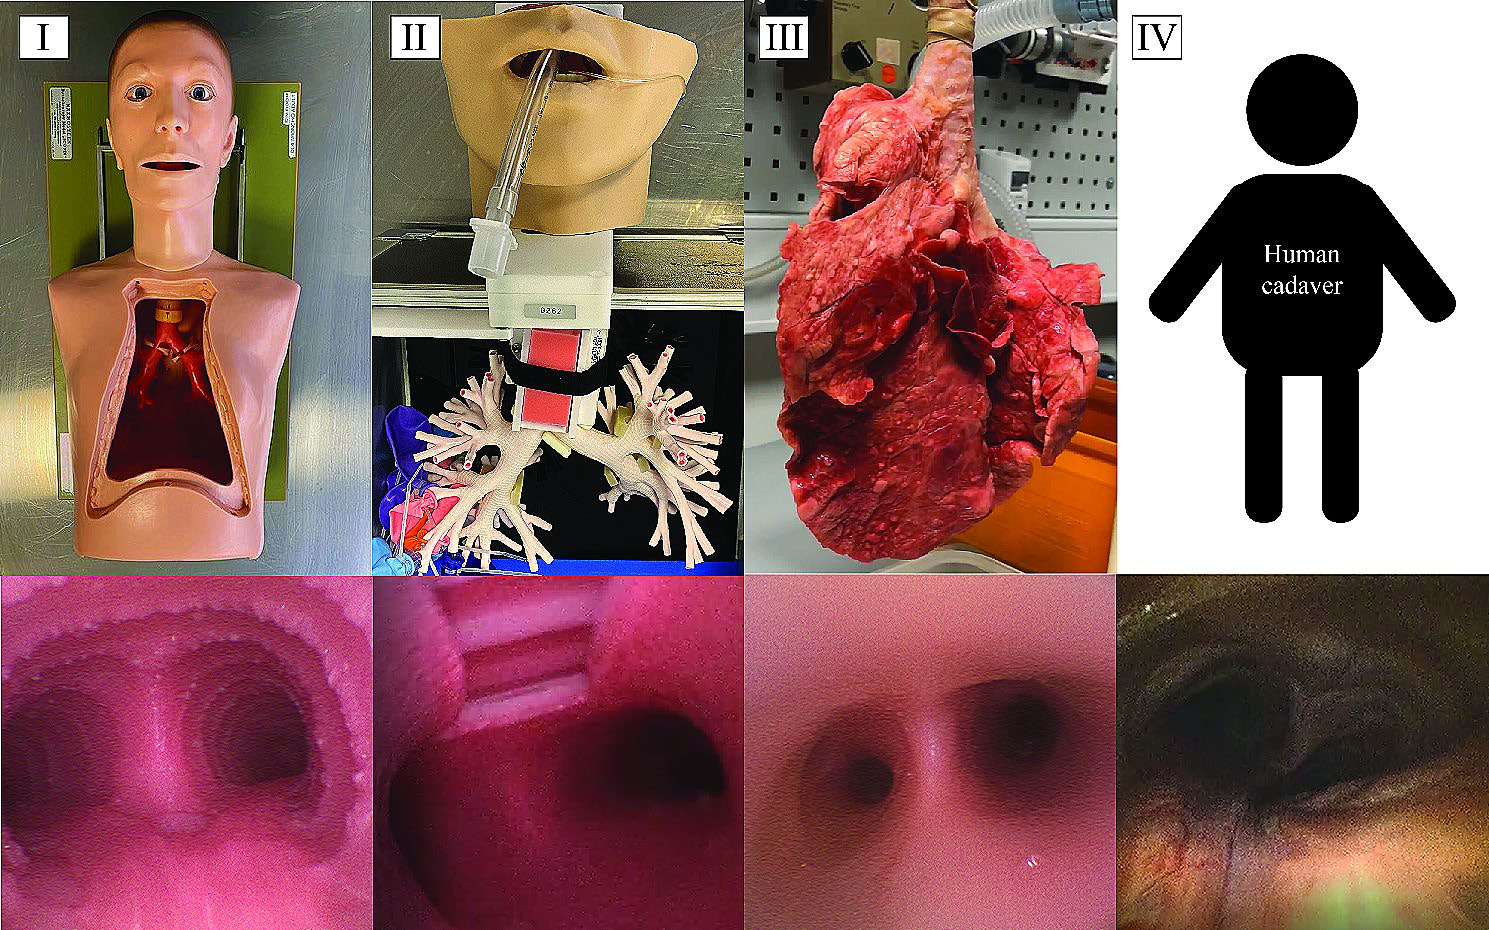
\includegraphics[width=0.86\textwidth]{artigos/modelos_treino_broncoscopia.png}
  \caption{Modelos de treino em broncoscopia \parencite{Kronborg2024}.}
  \label{fig:modelos-treino-broncoscopia}
\end{figure}

\section{Fidelidade dos simuladores}
A fidelidade de um simulador pode ser entendida em várias dimensões: 
\begin{itemize}
    \item Fidelidade anatómica $\rightarrow$ refere-se à correspondência entre a geometria do modelo e a anatomia real, como à forma, proporção e organização espacial das vias aéreas;
    \item Fidelidade mecânica $\rightarrow$ refere-se à resistência ao avanço, flexibilidade e resposta ao contacto; 
    \item Fidelidade funcional $\rightarrow$ refere-se à capacidade de reproduzir movimentos, variações de calibre e eventos transitórios como a tosse.
\end{itemize}

\begin{figure}[htbp]
  \centering
  \begin{tikzpicture}[
    axis/.style={draw, rounded corners=4pt, align=center, minimum width=3.8cm, minimum height=1.2cm, font=\small, thick},
    arr/.style={-Latex, thick}
  ]
    \node[axis, fill=blue!8] (anat) {Fidelidade\\anatómica};
    \node[axis, fill=green!10, right=1.0cm of anat] (mec) {Fidelidade\\mecânica};
    \node[axis, fill=orange!12, right=1.0cm of mec] (func) {Fidelidade\\funcional};
    \node[draw, rounded corners=5pt, align=center, below=1.0cm of mec, minimum width=5.0cm, minimum height=1.0cm, fill=gray!10] (treino) {Valor pedagógico\\do simulador};
    \draw[arr] (anat.south) -- (treino.north west);
    \draw[arr] (mec.south) -- (treino.north);
    \draw[arr] (func.south) -- (treino.north east);
  \end{tikzpicture}
  \caption{Dimensões de fidelidade consideradas num simulador físico.}
  \label{fig:dimensoes-fidelidade}
\end{figure}

Esta distinção aproxima-se da lógica proposta por Miller para a avaliação de competências clínicas, que separa aquilo que um profissional sabe, sabe fazer, demonstra saber fazer e efetivamente faz na prática, situando os simuladores físicos precisamente na transição entre o demonstrar e o fazer \parencite{Witheridge2019}. Importa, no entanto, notar que a relação entre fidelidade e aprendizagem não é necessariamente linear, havendo trabalhos recentes que questionam se um maior realismo se traduz sempre em mais competência adquirida, sugerindo que o envolvimento ativo do formando pode pesar tanto quanto o rigor da réplica anatómica \parencite{Pico2026}.

Na broncoscopia, um modelo estático pode ser útil para situações de treinos iniciais de navegação e reconhecimento anatómico. No entanto, durante um procedimento real, o operador encontra-se num ambiente vivo e dinâmico, em constante movimento. A respiração, os batimentos cardíacos, a tosse, a sedação e a própria interação do broncoscópio com as paredes internas exercem comportamentos e reações que modificam continuamente o ambiente e a sensação de controlo. Esta diferença cria oportunidade para os simuladores físicos de baixo custo que incorporem movimentos e fisiologia de forma controlada \parencite{Davoudi2008,Nilsson2017,Fu2023}.

\section{Simuladores de broncoscopia}
Os atuais simuladores de broncoscopia recorrem a vários tipos de sistemas, nomeadamente treinos em ambientes puramente virtuais, em manequins comerciais, em modelos de bancada e, mais recentemente, em modelos impressos em 3D.

Os sistemas virtuais, como o simulador ORSIM, permitem gerar cenários de dificuldade variável e obter métricas automáticas de desempenho, tendo demonstrado boa validade e fiabilidade na avaliação de competências em broncoscopia flexível, distinguindo de forma consistente entre principiantes e peritos \parencite{Baker2016}. Contudo, estes sistemas dependem de hardware háptico dedicado para simular a resistência ao avanço e o contacto com as paredes das vias aéreas, um aspeto que continua a ser tecnicamente difícil de reproduzir com fidelidade, uma vez que a deteção de força na interação entre instrumento e tecido em endoscopia minimamente invasiva (termo mais abrangente, que inclui a broncoscopia como um dos seus procedimentos) permanece uma área ativa de investigação, sem uma solução consensual e amplamente adotada \parencite{Hosseinabadi2021}. Modelos físicos baseados em tecido biológico real, como um biosimulador reutilizável construído a partir de pulmões suínos ventilados, procuram contornar esta limitação ao oferecer uma resposta tátil genuína, tendo sido avaliados favoravelmente por broncoscopistas experientes e principiantes em comparação direta com um simulador virtual comercial \parencite{Garner2019}. Estes modelos biológicos, no entanto, não são reutilizáveis indefinidamente, exigem preservação especializada e apresentam variabilidade anatómica de espécime para espécime, o que limita a sua padronização enquanto ferramenta de ensino e de avaliação objetiva.

Esta lacuna, entre a normalização própria dos sistemas virtuais e o realismo tátil dos modelos biológicos, abre espaço para os modelos impressos em 3D, que procuram oferecer geometria anatómica consistente e reprodutível, associada a materiais capazes de aproximar a resposta mecânica dos tecidos reais.

\begin{figure}[H]
  \centering
  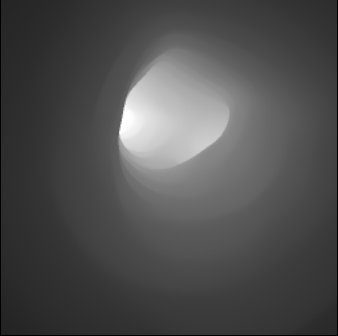
\includegraphics[width=0.74\textwidth]{artigos/broncoscopia_virtual_dunnbeltran.png}
  \caption{Exemplo de simulação virtual em broncoscopia \parencite{DunnBeltran2026}.}
  \label{fig:broncoscopia-virtual-dunnbeltran}
\end{figure}

\begin{figure}[H]
  \centering
  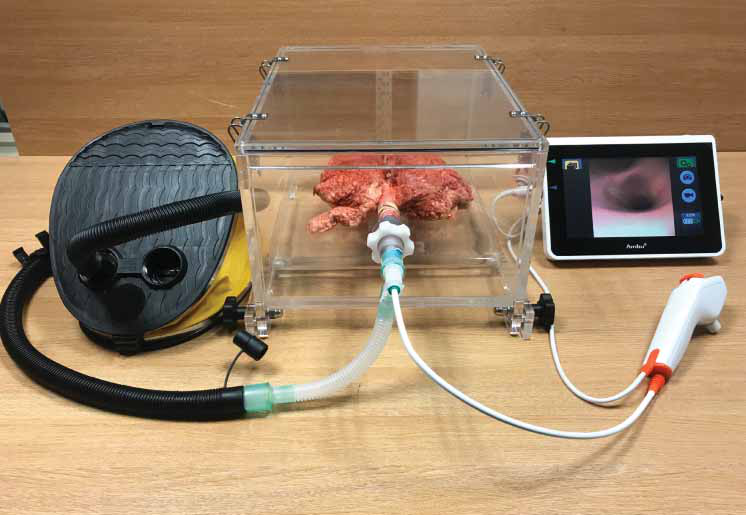
\includegraphics[width=0.76\textwidth]{artigos/simulador_biologico_garner.png}
  \caption{Biossimulador para treino de broncoscopia \parencite{Garner2019}.}
  \label{fig:simulador-biologico-garner}
\end{figure}

\section{Impressão 3D aplicada à simulação médica}
A impressão 3D é uma tecnologia de produção de objetos tridimensionais, realizada através da adição de material camada a camada, podendo o método de adição ou aglomeração dos materiais variar bastante consoante a tecnologia utilizada, entre as quais se destacam o FDM, a SLA e a SLS, cada uma assente num princípio de fabrico distinto e, por isso, mais adequada a diferentes tipos de aplicação.
Com o passar dos anos e o amadurecimento da tecnologia e dos materiais disponíveis, este método de produção veio proporcionar uma oportunidade inovadora na criação de estruturas e geometrias complexas, a um baixo custo e numa fração do tempo face aos outros métodos de produção, afetando todas as áreas científicas e industriais, incluindo a medicina. Esta permite a produção de protótipos anatómicos com custo relativamente baixo, a correção e o ajuste de dimensões em pouco tempo e o teste de materiais inovadores que, com outros métodos, seria impensável, tanto pelo custo de produção como pela complexidade dos processos.

\subsection{Técnicas de impressão 3D}
\label{subsec:tecnicas-impressao-3d}
O FDM (Fused Deposition Modeling, ou modelação por deposição de material fundido) é a tecnologia mais acessível e mais difundida, consistindo na extrusão de um filamento termoplástico aquecido através de um bico, que deposita o material camada a camada sobre uma base de impressão. É compatível com uma grande variedade de materiais, como o PLA, o PETG, o ABS ou filamentos flexíveis como o TPU, permitindo a produção de peças estruturalmente resistentes a um custo reduzido, ainda que com uma resolução e um acabamento de superfície mais limitados, sendo geralmente visíveis as linhas de cada camada. Para geometrias com zonas em consola ou sem apoio inferior, o FDM necessita ainda de estruturas de suporte, que têm de ser removidas após a impressão.

A SLA (Stereolithography) recorre a uma cuba de resina fotopolimérica líquida, curada seletivamente camada a camada por uma fonte de luz ultravioleta, um laser ou um projetor. Esta tecnologia permite obter peças com elevada resolução e um acabamento de superfície muito mais fino do que o FDM, sendo por isso indicada para modelos com geometrias detalhadas. Em contrapartida, exige equipamento de pós-processamento dedicado, nomeadamente para lavagem das peças em álcool isopropílico e cura adicional sob luz ultravioleta, além de recorrer a materiais mais dispendiosos e, em geral, mais frágeis do que os filamentos termoplásticos.

Por fim, a SLS (Selective Laser Sintering) utiliza um laser para sinterizar seletivamente um material em pó, tipicamente uma poliamida, camada a camada dentro de um leito de pó. Uma das suas principais vantagens é dispensar estruturas de suporte dedicadas, uma vez que o próprio pó não sinterizado sustenta as zonas em consola durante a impressão, permitindo fabricar geometrias mais complexas. As peças resultantes apresentam ainda propriedades mecânicas mais uniformes do que as obtidas por FDM. Contudo, o equipamento e os materiais são substancialmente mais caros, o que torna esta tecnologia mais comum em contexto industrial do que em pequenos projetos ou protótipos.

No contexto deste projeto, esta comparação foi particularmente relevante na escolha entre FDM e SLA para a impressão da árvore brônquica, decisão discutida em detalhe na \cref{sec:disposicao-impressao}.

A utilização clínica e educativa da impressão 3D em modelos anatómicos exige, contudo, um controlo de qualidade rigoroso ao longo de todo o processo, desde a segmentação da imagem médica até à impressão final, sendo possível identificar e quantificar erros próprios de cada etapa, como o erro de segmentação, o erro de edição digital e o erro de impressão propriamente dito, cuja soma determina a fidelidade geométrica final do modelo obtido \parencite{Schulze2024}. Esta preocupação com o rigor dimensional não se limita a modelos de treino, estendendo-se também a aplicações clínicas diretas, como o desenho e o fabrico de stents personalizados para o tratamento de estenoses das vias aéreas, benignas ou malignas, a partir da anatomia específica de cada doente \parencite{Aravena2023,Yilmaz2022,Shan2019}, ou ainda à produção de modelos de traqueia para treino de cricotiroidotomia de emergência e de modelos de vias aéreas superiores para treino de entubação endotraqueal, ambos criados com o objetivo de tornar este tipo de treino mais acessível e menos dependente de equipamento comercial dispendioso \parencite{Doucet2017,Park2023}.

\begin{figure}[htbp]
  \centering
  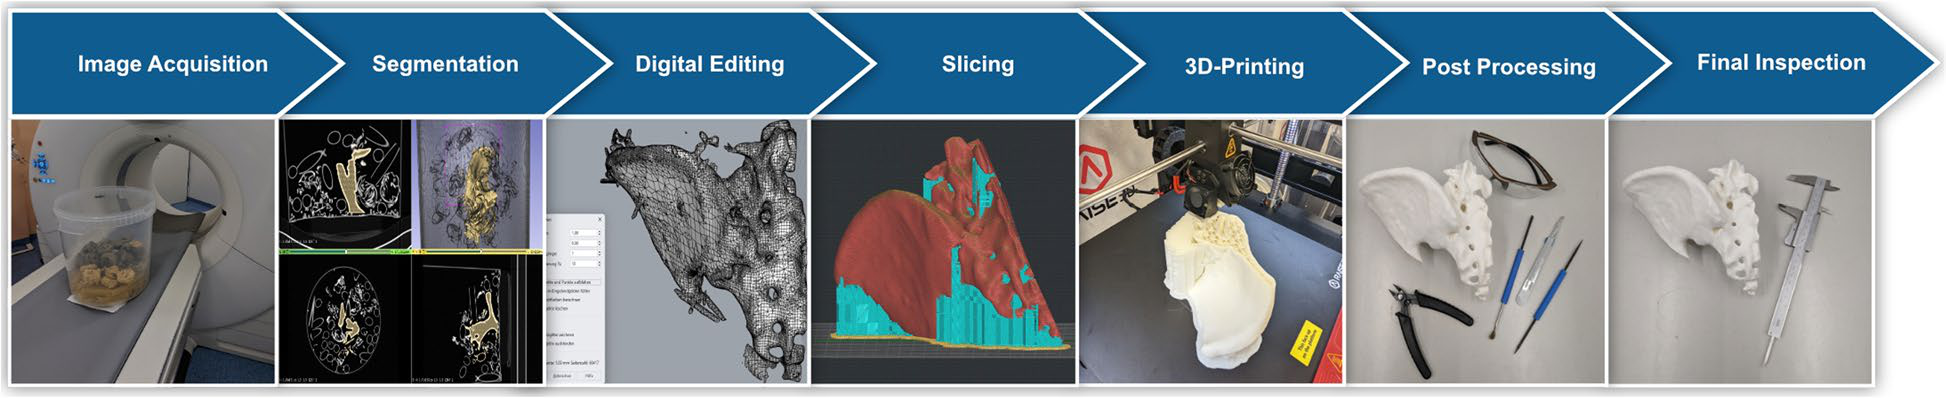
\includegraphics[width=0.92\textwidth]{artigos/workflow_modelos_3d.png}
  \caption{Fluxo de produção e validação de modelos anatómicos impressos em 3D \parencite{Schulze2024}.}
  \label{fig:workflow-modelos-3d}
\end{figure}

\subsection{Aplicação em simuladores de árvores brônquicas}
No caso dos simuladores de árvores brônquicas, os modelos impressos em 3D ganharam uma grande importância por permitirem transformar dados anatómicos, obtidos por exemplo a partir de exames de tomografia computorizada (TAC), em geometrias físicas. Em broncoscopia, esta abordagem pode representar a árvore traqueobrônquica com boa correspondência espacial e permitir a criação de simuladores específicos para treino de navegação \parencite{Pedersen2017,Fu2023}, ainda que a sua principal limitação, quando usados de forma isolada, seja a ausência de movimento e de resposta fisiológica. Modelos multi-material, combinando simultaneamente componentes rígidos e flexíveis numa só impressão, têm vindo a ser explorados precisamente para aproximar a experiência tátil da broncoscopia real sem comprometer a robustez estrutural do conjunto \parencite{Ho2019}, enquanto outras abordagens recorrem à impressão a cores, atribuindo uma cor distinta a cada segmento ou ramo brônquico, de modo a tornar mais percetível a organização da árvore traqueobrônquica e a facilitar simultaneamente o treino de navegação e a aprendizagem da nomenclatura anatómica \parencite{Leba2023}.

\begin{figure}[htbp]
  \centering
  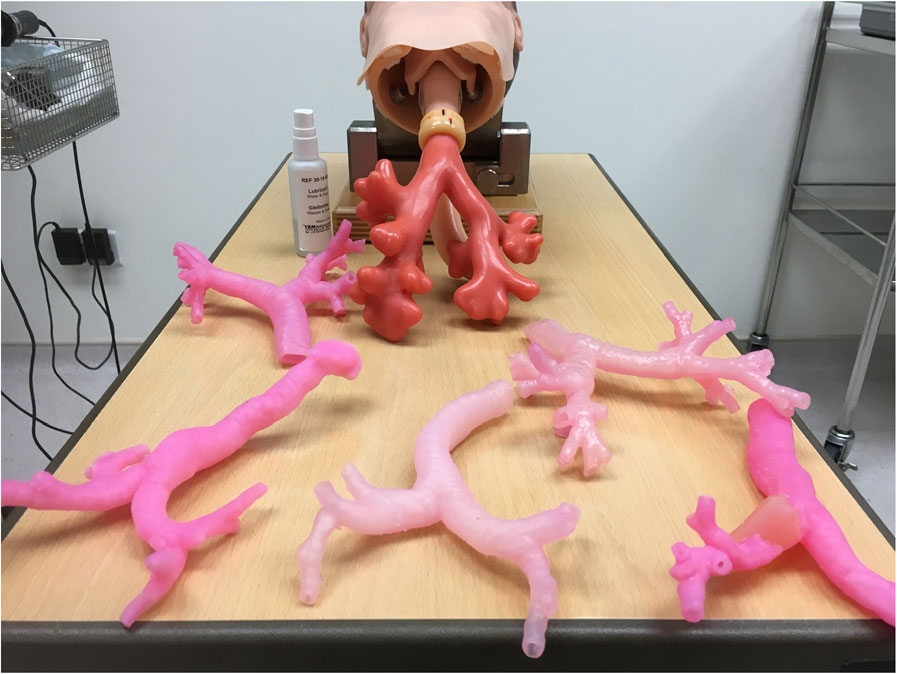
\includegraphics[width=0.74\textwidth]{artigos/modelos_multimaterial_broncoscopia.png}
  \caption{Modelos brônquicos impressos em multi-material \parencite{Ho2019}.}
  \label{fig:modelos-multimaterial-broncoscopia}
\end{figure}

Além dos modelos multi-material, existem abordagens que exploram a cor e o planeamento personalizado para tornar a anatomia mais legível ou adaptar o modelo a uma necessidade clínica concreta.

\begin{figure}[H]
  \centering
  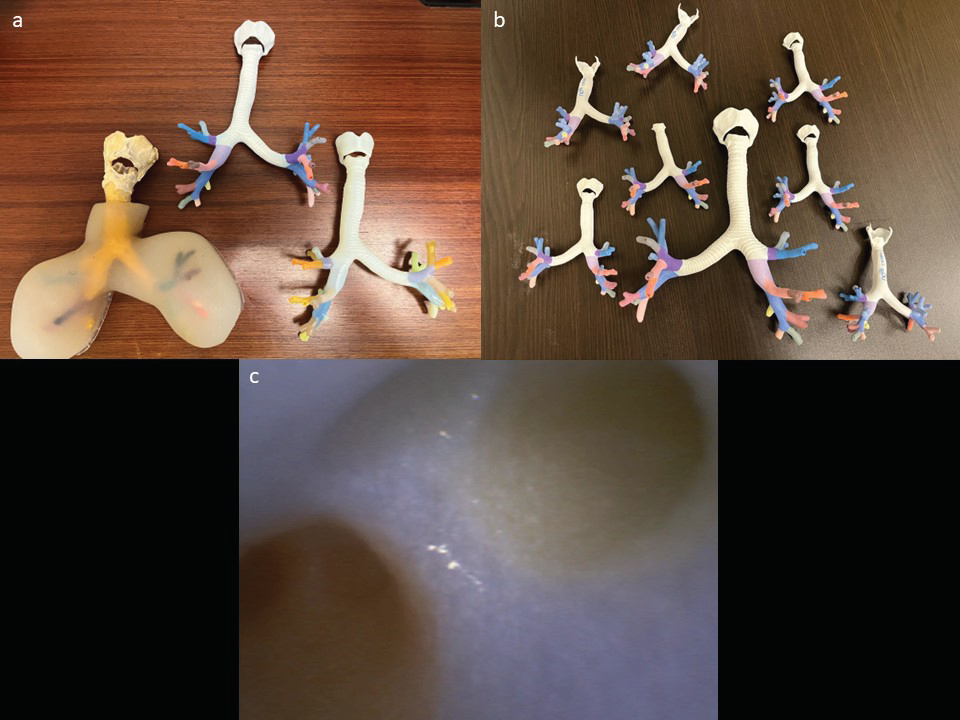
\includegraphics[width=0.68\textwidth]{artigos/modelo_vias_colorizado.png}
  \caption{Modelo de vias aéreas segmentado por cor \parencite{Leba2023}.}
  \label{fig:modelo-vias-colorizado}
\end{figure}

Contudo, a ideia de impressão destes modelos apresenta desafios e detalhes muito importantes, tais como a escolha do material, pois facilmente influencia o grau de dificuldade de impressão, a flexibilidade, a resistência, a sensação ao toque e a disponibilidade de cor. Materiais rígidos podem servir para validar forma e montagem, enquanto materiais flexíveis podem aproximar-se melhor à resposta mecânica, ainda que aumentem consideravelmente a dificuldade de impressão e calibração. Assim, a impressão 3D deve ser entendida também como uma plataforma de iteração, não apenas como uma técnica de fabrico final.

\begin{figure}[H]
  \centering
  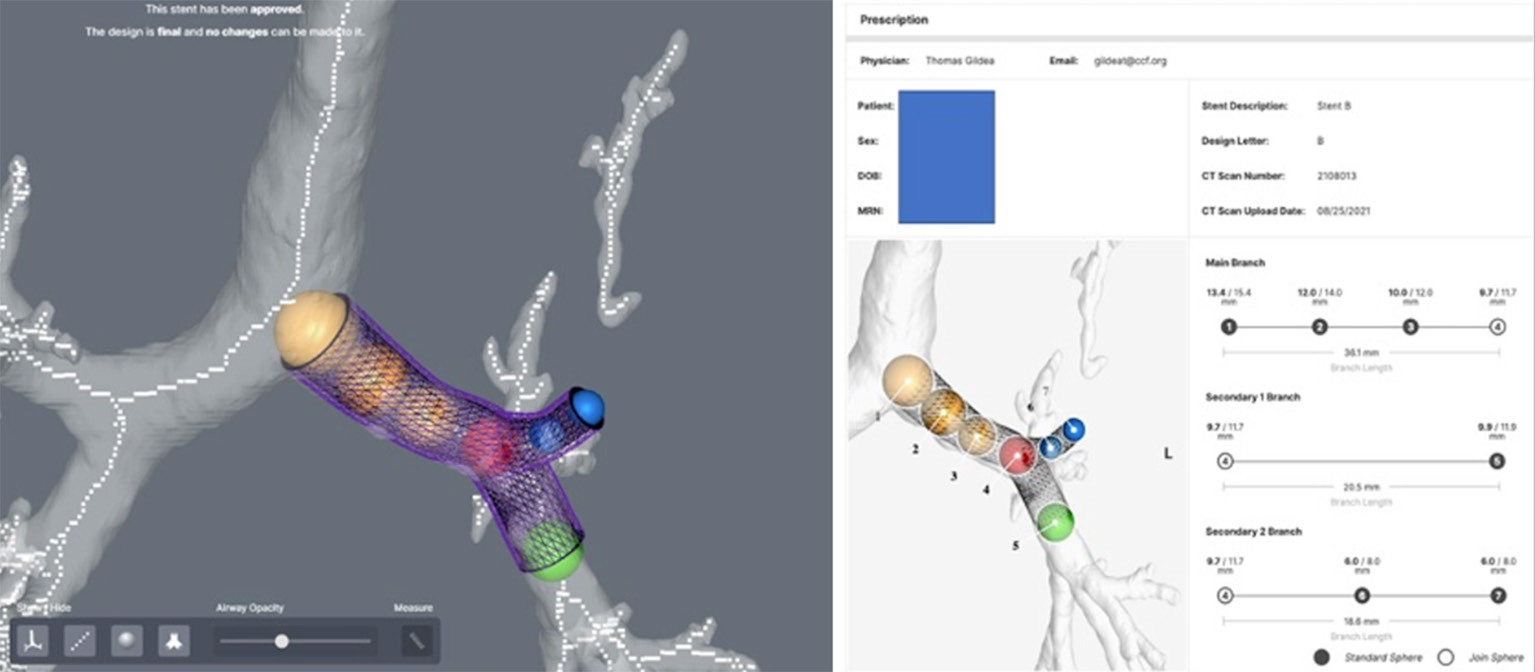
\includegraphics[width=0.62\textwidth]{artigos/stent_aereo_personalizado.png}
  \caption{Planeamento de stent personalizado para vias aéreas \parencite{Aravena2023}.}
  \label{fig:stent-aereo-personalizado}
\end{figure}

\section{Movimentos observáveis durante a broncoscopia}
A árvore traqueobrônquica não se comporta como uma estrutura fixa durante uma broncoscopia. Mesmo quando o broncoscópio se mantém praticamente parado, a imagem observada pode apresentar deslocações lentas, alterações de orientação, variações do lúmen e perturbações rápidas. 
Para o operador, estes movimentos não aparecem isolados: 
\begin{itemize}
    \item A respiração cria uma componente periódica dominante;
    \item O batimento cardíaco acrescenta pequenas oscilações locais;
    \item A tosse introduz eventos abruptos;
    \item O contacto do broncoscópio com a parede pode modificar temporariamente a posição ou a forma do segmento observado.
\end{itemize}

Do ponto de vista de um simulador físico, estes fenómenos não precisam de ser reproduzidos com toda a complexidade fisiológica para terem valor pedagógico, mesmo que acabem sempre por apresentar um maior realismo. O mais importante é que o utilizador deixe de observar um modelo completamente estático e passe a treinar num ambiente com movimento por vezes imprevisível e suficientemente coerente com o que é visto durante o procedimento real. Por isso, os movimentos descritos de seguida foram analisados quanto à sua relevância visual, dificuldade de implementação e utilidade, seguindo a categorização e os intervalos de frequência e amplitude propostos num documento de trabalho elaborado especificamente para este projeto pela equipa de Pneumologia do Centro Hospitalar Universitário do Algarve \parencite{Santos2026}, que serviu de base clínica direta às secções seguintes.

\subsection{Movimento respiratório}
O movimento respiratório é a componente mais frequente e previsível, ocorrendo durante o processo cíclico da inspiração e expiração, descrito como a deslocação dos pulmões com predominância craniocaudal, acompanhado por pequenas componentes laterais e por alterações locais da geometria das vias aéreas. A frequência respiratória normal situa-se aproximadamente entre 12 e 20 ciclos por minuto, embora possa variar com ansiedade, sedação, esforço respiratório, patologia e contexto clínico.

Análises mostram que a fase respiratória pode alterar a posição de estruturas pulmonares e influenciar modelos de fluxo nas vias aéreas \parencite{Chen2015,Gunatilaka2020}, existindo ainda, além da deslocação global, variações do calibre brônquico ao longo do ciclo respiratório, um fenómeno já descrito por trabalhos clássicos que demonstraram os mecanismos das alterações de calibre dos brônquios durante a respiração normal e das suas variações rítmicas \parencite{Heinbecker1927,Ellis1936}. Mais recentemente, técnicas de modelação computacional têm procurado prever e simular este movimento de forma específica ao paciente, recorrendo a modelos de elementos finitos capazes de estimar o deslocamento dos brônquios ao longo do ciclo respiratório a partir de imagem médica, alcançando erros de previsão inferiores a 3\% quando validados com dados reais \parencite{Kim2023}. Para o protótipo desenvolvido, esta componente foi interpretada como um movimento lento e periódico, adequado para ser representado por trajetórias sinusoidais, suaves e repetíveis.

\begin{figure}[htbp]
  \centering
  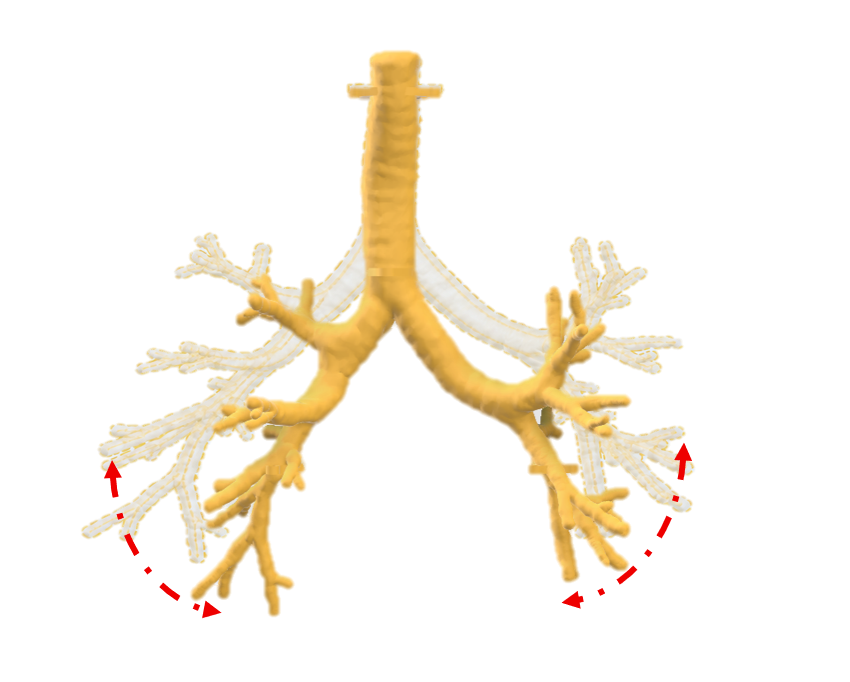
\includegraphics[width=0.62\textwidth]{fotos/movimento_respiratorio_arvore.png}
  \caption{Representação esquemática do movimento respiratório da árvore brônquica.}
  \label{fig:movimento-respiratorio-arvore-estado-arte}
\end{figure}

\begin{figure}[htbp]
  \centering
  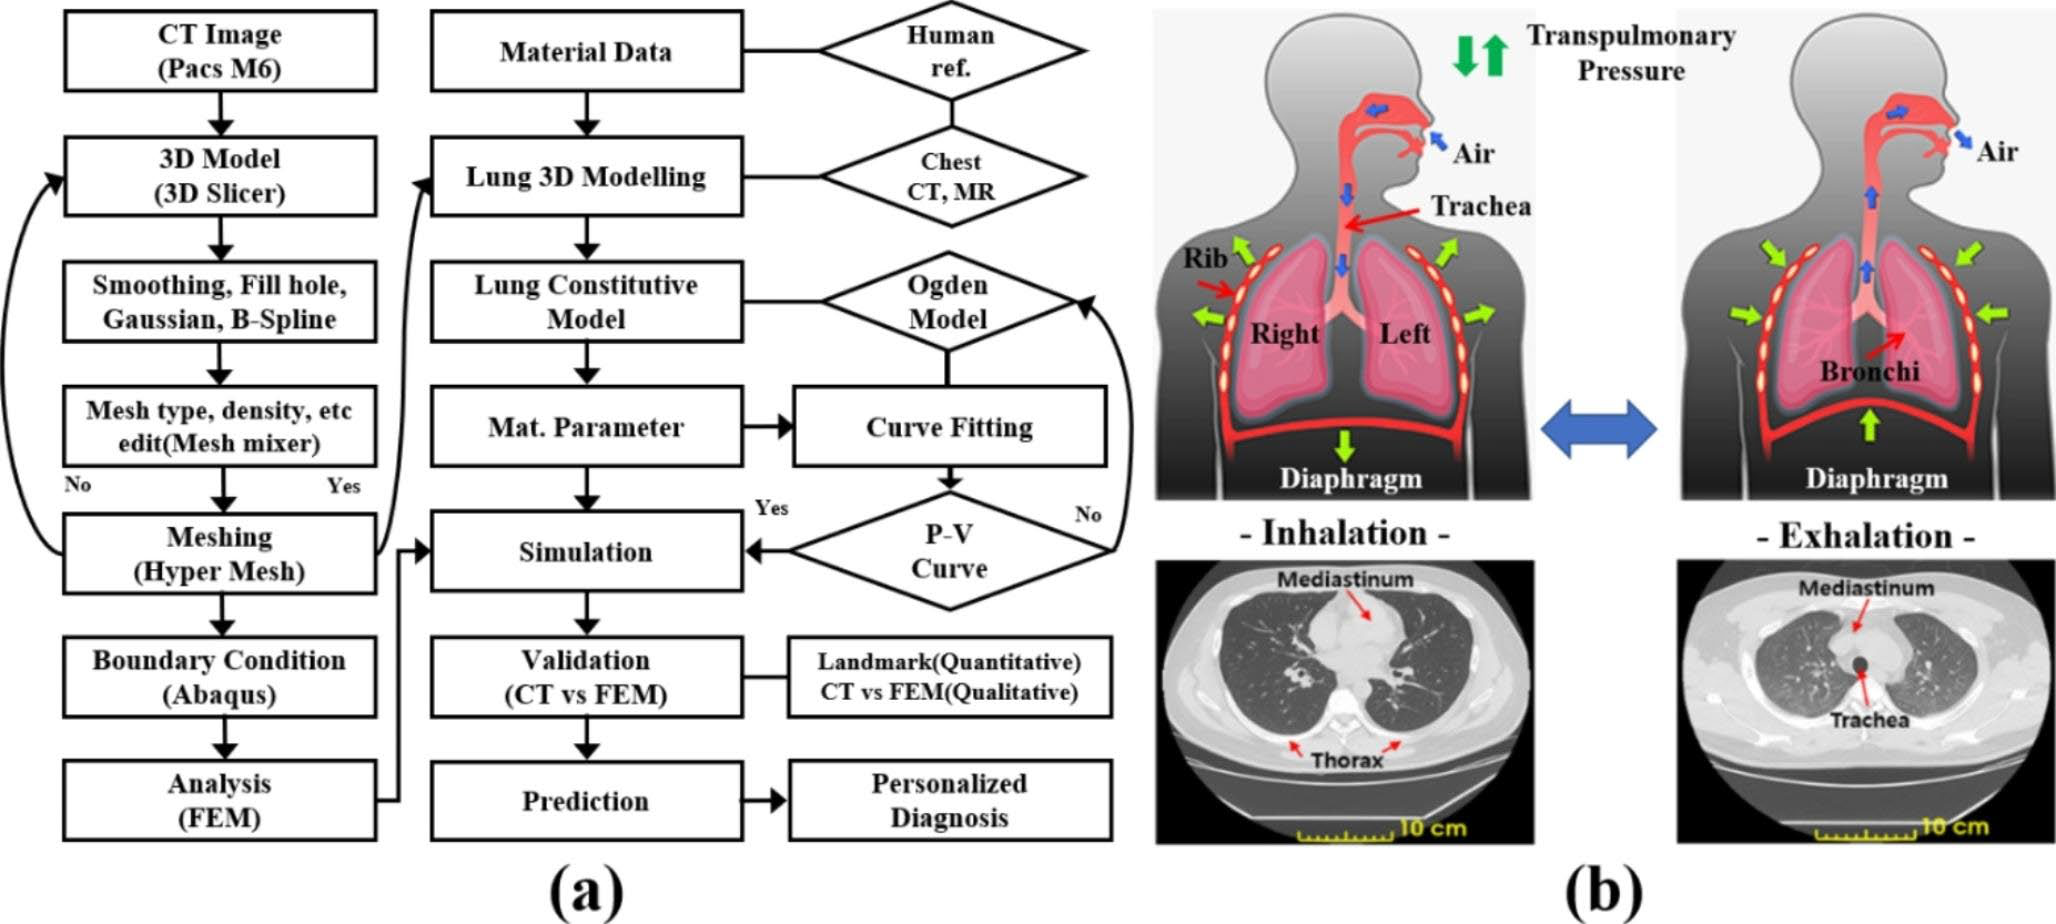
\includegraphics[width=0.88\textwidth]{artigos/modelo_movimento_respiratorio_kim.png}
  \caption{Modelo computacional do movimento respiratório \parencite{Kim2023}.}
  \label{fig:modelo-movimento-respiratorio-kim}
\end{figure}

\subsection{Movimento cardíaco}
O movimento cardíaco introduz oscilações mais rápidas e de menor amplitude, com intervalos regulares entre ocorrências, cuja influência tende a ser mais percetível em regiões próximas do coração, em particular junto ao brônquio principal esquerdo e a estruturas adjacentes. Ao contrário da respiração, que domina a posição global da árvore brônquica, o batimento cardíaco surge antes como uma vibração ou perturbação sobreposta.

Estudos com imagem 4D confirmam esta distinção, tendo quantificado separadamente as contribuições respiratória e cardíaca no movimento de estruturas pulmonares e observado uma influência cardíaca proporcionalmente maior em lesões centrais e superiores, mais próximas do coração e dos grandes vasos \parencite{Savanovic2023}. Esta influência não se limita à posição da árvore brônquica, estendendo-se também ao próprio fluxo de ar no seu interior. Imagem dinâmica obtida por radiação de sincrotrão revelou que o batimento cardíaco gera oscilações de pressão e de fluxo de ar mensuráveis nos brônquios principais, num fenómeno localizado junto à carina até então difícil de demonstrar experimentalmente \parencite{Dubsky2018}. Em casos anatómicos particulares, esta proximidade pode mesmo traduzir-se em compressão mecânica direta do brônquio principal esquerdo por estruturas cardiovasculares adjacentes, como a aorta descendente ou uma artéria pulmonar dilatada, um efeito documentado em população pediátrica com anomalias intracardíacas \parencite{Ando2024}.

\begin{figure}[htbp]
  \centering
  \begin{tikzpicture}[
    x=0.9cm,
    y=1.0cm,
    axis/.style={gray!55, thin},
    ecg/.style={red!70!black, very thick, line join=round, line cap=round},
    lab/.style={font=\small}
  ]
    \foreach \x in {0,...,12} {
      \draw[axis] (\x,-0.8) -- (\x,1.7);
    }
    \foreach \y in {-0.5,0,0.5,1,1.5} {
      \draw[axis] (0,\y) -- (12,\y);
    }
    \draw[ecg]
      (0,0) -- (0.6,0) .. controls (0.8,0.15) and (1.0,0.15) .. (1.2,0)
      -- (1.7,0) -- (1.9,-0.35) -- (2.1,1.55) -- (2.3,-0.55) -- (2.55,0)
      -- (3.2,0) .. controls (3.6,0.45) and (4.0,0.45) .. (4.45,0)
      -- (5.4,0)
      .. controls (5.6,0.12) and (5.85,0.12) .. (6.05,0)
      -- (6.55,0) -- (6.75,-0.35) -- (6.95,1.45) -- (7.15,-0.5) -- (7.42,0)
      -- (8.1,0) .. controls (8.5,0.42) and (8.9,0.42) .. (9.35,0)
      -- (10.1,0)
      .. controls (10.3,0.12) and (10.55,0.12) .. (10.75,0)
      -- (11.25,0) -- (11.45,-0.3) -- (11.65,1.35) -- (11.82,-0.45) -- (12,0);
    \node[lab, red!70!black] at (2.1,1.85) {QRS};
    \node[lab] at (1.0,0.42) {P};
    \node[lab] at (3.8,0.72) {T};
    \draw[-Latex, thick] (2.1,-0.95) -- (2.1,-0.62);
    \draw[-Latex, thick] (6.95,-0.95) -- (6.95,-0.58);
    \draw[Latex-Latex, thick] (2.1,-1.12) -- node[below, font=\small] {período entre batimentos} (6.95,-1.12);
  \end{tikzpicture}
  \caption{Representação esquemática de um ciclo cardíaco através da onda de ECG.}
  \label{fig:ecg-batimento-cardiaco}
\end{figure}

Num modelo de treino, esta componente é útil para quebrar a sensação de movimento puramente sinusoidal e para acrescentar uma perturbação de menor amplitude, pelo que, no contexto deste projeto, o batimento cardíaco não foi tratado como uma reconstrução anatómica exata da interação coração-pulmão, mas antes como um perfil adicional de movimento, mais rápido e discreto, combinado com a respiração.

\subsection{Tosse e perturbações rápidas}
A tosse é um evento curto, abrupto e menos previsível, provocando, durante uma broncoscopia, a deslocação súbita das vias aéreas, com tendência para a ocorrência de réplicas adjacentes à deslocação principal, alteração temporária do campo visual, variação do fluxo de ar e perda momentânea de orientação. Para quem treina, este tipo de evento é importante porque obriga a recuperar a posição visual e a manter controlo do broncoscópio após uma perturbação.

A tosse é, em si mesma, um reflexo vital complexo, composto por uma fase inspiratória, uma fase compressiva com encerramento da glote e uma fase expiratória explosiva, coordenada por recetores das vias aéreas e por vias nervosas aferentes e eferentes bem descritas na literatura fisiológica \parencite{Andrani2018}. A modelação computacional recente deste fenómeno tem-se debruçado sobre a dinâmica de gotículas e da película mucosa nas vias aéreas superiores durante um evento de tosse, com o objetivo de relacionar as suas características com diferentes patologias pulmonares \parencite{Ilegbusi2025}, o que confirma o interesse científico atual em compreender este movimento para além da sua simples deteção visual durante um procedimento.

\begin{figure}[htbp]
  \centering
  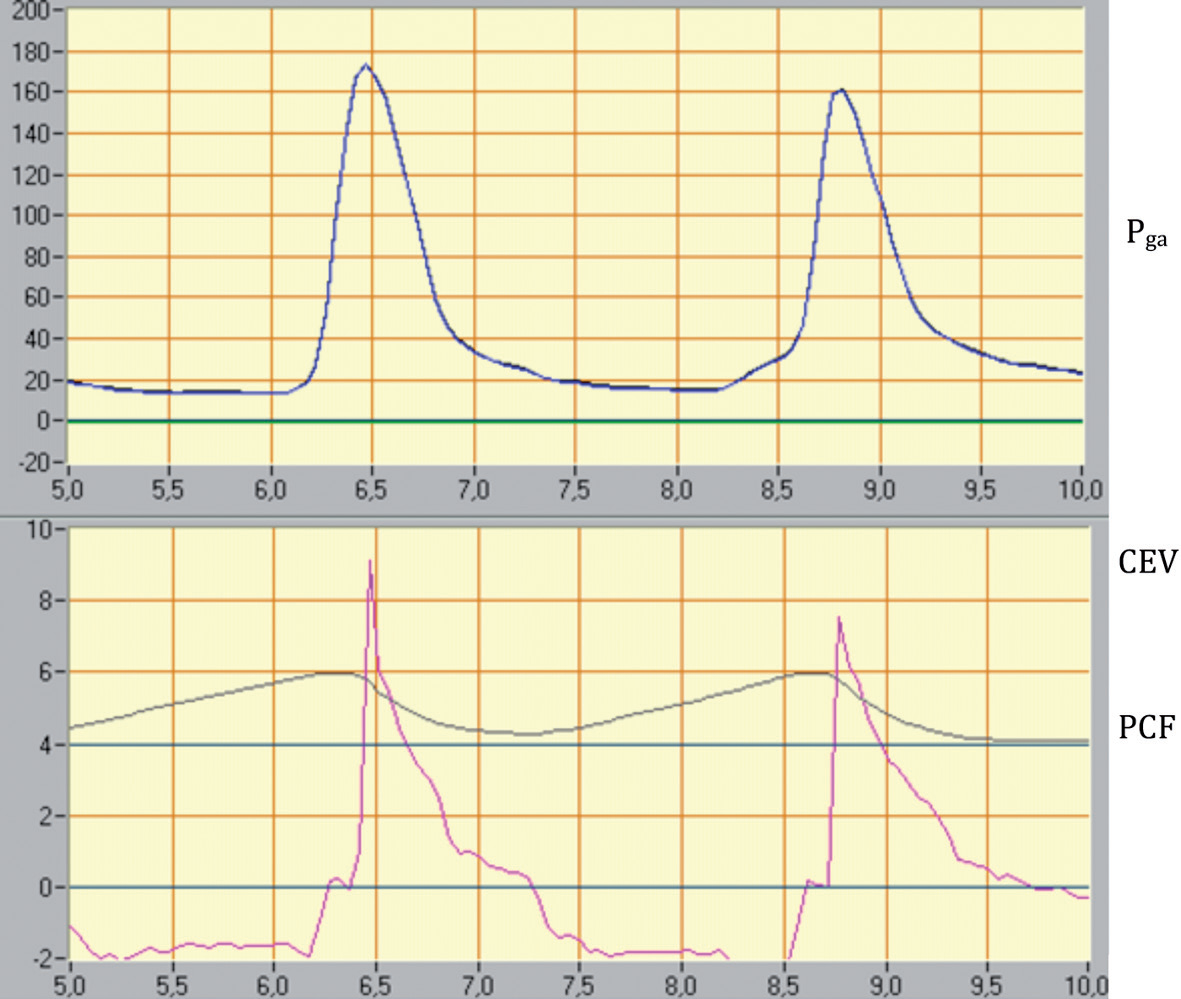
\includegraphics[width=0.72\textwidth]{artigos/tosse_pressao_andrani.png}
  \caption{Variação de pressão e fluxo durante o reflexo da tosse \parencite{Andrani2018}.}
  \label{fig:tosse-pressao-andrani}
\end{figure}

No simulador, a tosse deve por isso ser representada como um evento transitório, com duração reduzida e amplitude superior à do batimento cardíaco, podendo a sua ocorrência ser programada de forma aleatória dentro de limites definidos, o que permite criar cenários de treino mais realistas sem obrigar à reprodução completa da fisiologia da tosse.

\subsection{Interação com o broncoscópio}
A passagem do broncoscópio também influencia a geometria observada, dado que o contacto com as paredes pode causar deformações locais, resistência ao avanço, pequenas oscilações e alterações da orientação da imagem. Esta componente é especialmente importante para o realismo tátil, porque aproxima o simulador da sensação física de navegação no interior das vias aéreas.

Apesar da sua relevância, esta interação mostra-se a mais difícil de implementar, exigindo materiais flexíveis adequados, geometrias calibradas com espessura e resistência adequadas e, idealmente, sensores ou mecanismos capazes de responder ao contacto. Esta dificuldade é também reconhecida na investigação em robótica endoscópica (área mais ampla, da qual a robótica aplicada à broncoscopia faz parte), onde a deteção de força na interação entre instrumento e tecido continua a ser identificada como um dos principais

\begin{figure}[H]
  \centering
  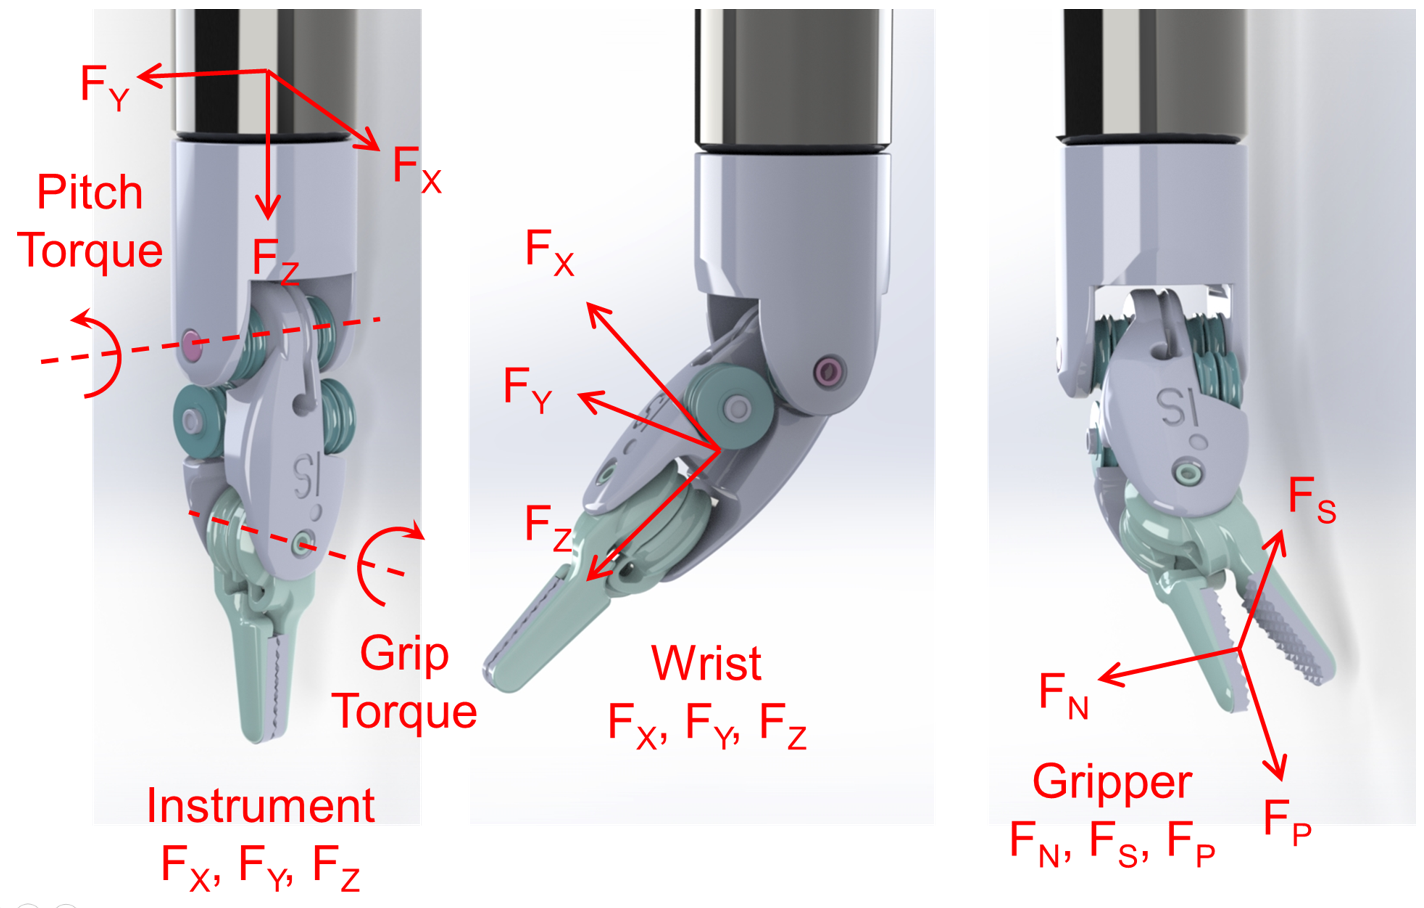
\includegraphics[width=0.70\textwidth]{artigos/forcas_endoscopia_hosseinabadi.png}
  \caption{Forças de contacto em endoscopia robótica \parencite{Hosseinabadi2021}.}
  \label{fig:forcas-endoscopia-hosseinabadi}
\end{figure}

desafios em cirurgia minimamente invasiva \parencite{Hosseinabadi2021}, tendo já sido exploradas soluções como broncoscópios robóticos de balão, especificamente concebidos para procedimentos nas vias aéreas e capazes de aplicar forças controladas sobre as suas paredes sem lesionar o tecido, ainda que este tipo de solução acrescente complexidade mecânica significativa ao sistema \parencite{Li2022}. Esta complexidade torna particularmente difícil a implementação deste tipo de fenómeno num simulador.

\begin{figure}[H]
  \centering
  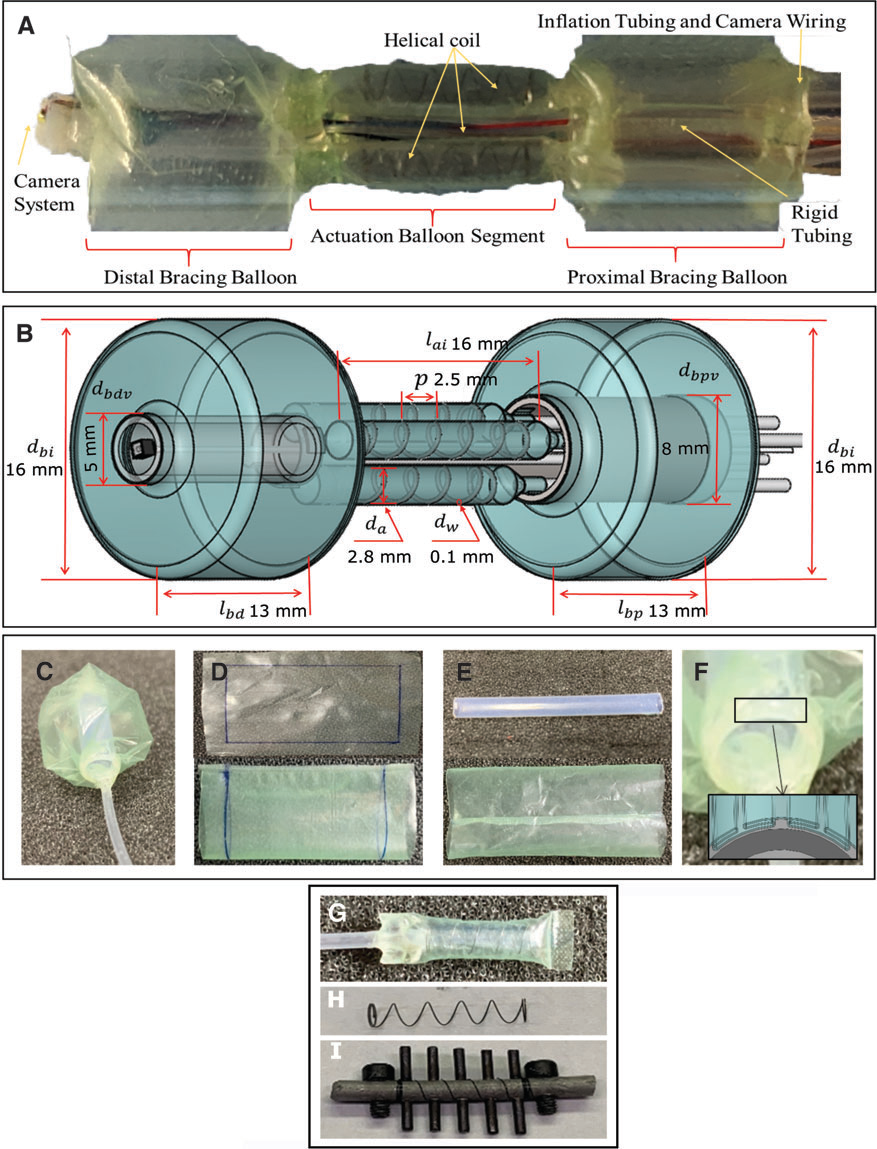
\includegraphics[width=0.70\textwidth]{artigos/broncoscopio_balao_li.png}
  \caption{Broncoscópio robótico com balão \parencite{Li2022}.}
  \label{fig:broncoscopio-balao-li}
\end{figure}

\subsection{Patologias e deformações locais}
Estenoses, obstruções, variações anatómicas e alterações patológicas modificam a navegação e o aspeto interno das vias aéreas, sendo que a impressão 3D permite criar geometrias específicas para representar alguns destes cenários de forma estática, o que já pode ser útil para treino de reconhecimento anatómico e planeamento de procedimentos. Um exemplo clínico bem documentado deste tipo de fenómeno é a traqueobroncomalácia, uma condição em que o amolecimento da cartilagem traqueal e brônquica provoca colapso dinâmico excessivo das vias aéreas, observado por videobroncoscopia em cerca de 69\% dos asmáticos com doença grave, contra apenas 1,6\% em indivíduos saudáveis \parencite{DalNegro2013}. Também a broncoconstrição ativa tem sido alvo de modelação matemática multiescala, procurando explicar como a complacência não linear da parede brônquica modula a resposta dinâmica das vias aéreas a estímulos broncoconstritores \parencite{Hiorns2014}.

No entanto, a simulação ativa de estenose variável, colapso local ou deformação dinâmica do lúmen exige um conjunto complexo de atuadores distribuídos, materiais compatíveis e uma estratégia de controlo mais complexa.

\begin{figure}[H]
  \centering
  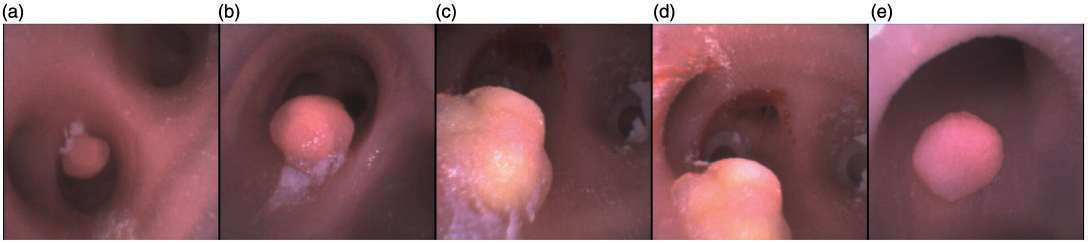
\includegraphics[width=0.66\textwidth]{artigos/modelo_dinamico_fu.png}
  \caption{Modelo impresso com expansão passiva por insuflação \parencite{Fu2023}.}
  \label{fig:modelo-dinamico-fu}
\end{figure}

\section{Síntese crítica}
Esta análise comprova que existem necessidades que nem sempre são satisfeitas em simultâneo. 
Por um lado, os simuladores devem ser suficientemente acessíveis para poderem ser usados em contexto académico e profissional, permitindo treinos repetidos.
Por outro, devem evitar uma representação demasiado estática das vias aéreas, porque a broncoscopia real ocorre num ambiente anatómico em constante movimento.

\begin{figure}[H]
  \centering
  \begin{tikzpicture}[
    box/.style={draw, rounded corners=4pt, align=center, minimum width=3.6cm, minimum height=1.2cm, font=\small, thick},
    arr/.style={-Latex, thick}
  ]
    \node[box, fill=gray!10] (static) {Modelos físicos\\estáticos};
    \node[box, fill=blue!8, right=0.8cm of static] (virtual) {Simulação\\virtual};
    \node[box, fill=orange!12, right=0.8cm of virtual] (dynamic) {Modelos com\\dinamismo parcial};
    \node[box, fill=green!12, below=1.1cm of virtual, minimum width=4.3cm] (gap) {Lacuna identificada:\\árvore brônquica física\\com atuação mecânica};
    \draw[arr] (static.south) -- (gap.west);
    \draw[arr] (virtual.south) -- (gap.north);
    \draw[arr] (dynamic.south) -- (gap.east);
  \end{tikzpicture}
  \caption{Posicionamento da lacuna identificada na literatura revista.}
  \label{fig:sintese-lacuna-literatura}
\end{figure}

Os modelos impressos em 3D respondem bem à primeira necessidade, pois permitem criar geometrias anatómicas de baixo custo e iterar rapidamente o projeto, como demonstram diversos exemplos comerciais e académicos de árvores brônquicas estáticas, alguns já disponíveis há várias décadas \parencite{Pedersen2017,Ho2019,Leba2023,Plan3DChile,TruCorpAirSim,PatUS5597310A}.
Contudo, quando usados isoladamente, tendem a limitar-se à fidelidade geométrica.

Algumas publicações têm procurado atenuar exatamente esta limitação, conferindo algum grau de dinamismo a modelos impressos em 3D e a outras réplicas físicas de vias aéreas, embora nenhuma delas recorra a atuação mecânica da própria estrutura anatómica. Um primeiro exemplo consiste na insuflação controlada de ar ou soro através de uma porta lateral, fazendo com que o próprio modelo impresso se expanda e contraia de forma passiva, uma solução já aplicada a um protótipo de via aérea impresso em 3D capaz de emular movimento fisiológico e patológico \parencite{Fu2023}. Outro trabalho, mais próximo da atuação robótica, recorre a seringas acionadas por uma guia linear motorizada para empurrar ar através de condutas rígidas que representam a árvore brônquica e a traqueia, replicando fisicamente tanto a respiração como a tosse. Contudo, mesmo nesta solução, os brônquios e a traqueia permanecem estruturas rígidas e estáticas, sendo apenas o fluxo de ar no seu interior que é mecanicamente controlado, sem qualquer tentativa de reproduzir o batimento cardíaco \parencite{Giannaccini2017}.

Fora do domínio da broncoscopia, outros trabalhos recorrem a atuação mecânica real para simular a mecânica ventilatória, mas fazem-no ao nível do diafragma ou da parede torácica, não da própria árvore brônquica. É o caso de um simulador respiratório que combina músculos artificiais pneumáticos com um diafragma sintético para insuflar pulmões reais ou artificiais \parencite{Horvath2020}, de um simulador eletromecânico de pulmão que combina componentes poliméricos e tecido pulmonar orgânico para reproduzir uma respiração realista \parencite{Pare2019} e de modelos deformáveis usados em radioterapia para replicar mecanicamente a expansão e a contração de um pulmão, sem qualquer representação da árvore brônquica no seu interior \parencite{Chang2010}. À mesma categoria pertencem ainda simuladores pulmonares controlados por motor de passo ou por pistão servo-controlado, desenvolvidos sobretudo para testar e calibrar ventiladores mecânicos \parencite{Zhao2025,PatUS5975748A}, bem como patentes que atuam mecanicamente a parede torácica de manequins de treino, por bolsas de ar ou por sistemas biela-manivela, para simular respiração ou manobras de reanimação \parencite{PatCN101447141B,PatEP2430628B1}. Outros dispositivos comerciais patenteados representam a árvore brônquica de forma mais completa, incluindo canais para brônquio esquerdo, direito e traqueia, mas destinam-se a treinar procedimentos de drenagem postural com sensores de posição, não a reproduzir movimento fisiológico \parencite{PatCN107346634B}. Uma última categoria de dispositivos recorre efetivamente a atuadores mecânicos reais sobre estruturas anatómicas de treino, mas aplicados à via aérea superior, como a mandíbula, a língua ou a articulação temporomandibular em simuladores de gestão de via aérea e de entubação orotraqueal, nunca chegando a atuar a árvore brônquica em profundidade e as suas bifurcações \parencite{TakanishiWKA}.

Do lado puramente computacional, têm também sido propostos métodos capazes de simular visualmente a deformação respiratória das vias aéreas durante a navegação broncoscópica, por renderização de imagem em tempo real a partir de dados de tomografia computorizada, as imagens médicas que descrevem em cortes transversais a anatomia interna do paciente, mas sem qualquer correspondência física. O resultado é sempre uma simulação gráfica, não um modelo tangível que o formando possa manipular com um broncoscópio real \parencite{DunnBeltran2026}. Já no campo da robótica cirúrgica aplicada à broncoscopia, os poucos manipuladores desenvolvidos destinam-se a operar sobre vias aéreas reais de doentes ou de cadáveres, como ferramentas de tratamento e não como modelos de treino, permanecendo a anatomia sempre estática durante a sua atuação \parencite{Gafford2019}. Mesmo alargando esta análise a protótipos ibero-americanos, como um simulador de broncoscopia com realimentação háptica desenvolvido no México, cuja árvore brônquica nunca chega a ser impressa fisicamente e permanece apenas como um modelo gráfico renderizado \parencite{IPN2012}, a conclusão mantém-se a mesma.

Em síntese, não se encontrou em toda a literatura revista nenhum modelo de árvore brônquica impresso em 3D em que a própria estrutura anatómica seja mecanicamente atuada, por manipuladores robóticos ou mecanismo equivalente, de forma a reproduzir de forma simultânea os principais fenómenos fisiológicos observáveis durante a broncoscopia. É precisamente esta lacuna que o presente projeto procura preencher.

\begin{figure}[H]
  \centering
  \begin{tikzpicture}[
    block/.style={draw, rounded corners=4pt, align=center, minimum height=1.0cm, font=\small, thick},
    arr/.style={-Latex, thick}
  ]
    \node[block, fill=blue!8, minimum width=3.1cm] (anat) {Fidelidade\\anatómica};
    \node[block, fill=orange!12, right=0.55cm of anat, minimum width=3.1cm] (mov) {Movimento\\fisiológico};
    \node[block, fill=green!12, right=0.55cm of mov, minimum width=3.1cm] (cost) {Acessibilidade\\e repetição};
    \node[block, fill=gray!10, below=1.0cm of mov, minimum width=5.6cm] (proj) {Objetivo do projeto\\modelo físico dinâmico};
    \draw[arr] (anat.south) -- (proj.north west);
    \draw[arr] (mov.south) -- (proj.north);
    \draw[arr] (cost.south) -- (proj.north east);
  \end{tikzpicture}
  \caption{Critérios reunidos na proposta desenvolvida.}
  \label{fig:sintese-criterios-projeto}
\end{figure}

A componente dinâmica, mesmo que simplificada, acrescenta valor ao treino, pois obriga o utilizador a lidar com deslocações por vezes imprevisíveis e com a perda parcial do enquadramento, devido a perturbações temporárias.

Assim, o objetivo deste projeto encontra-se em combinar uma árvore brônquica física, obtida por impressão 3D, com uma arquitetura de atuação capaz de reproduzir de forma controlada os fenómenos anatómicos dinâmicos identificados ao longo deste capítulo, respondendo a uma lacuna que a literatura revista ainda não preenche.

\chapter{Desenvolvimento do Hardware}

Este capítulo documenta a fase que ocupou a primeira metade do tempo dedicado a este projeto e que serviu de alicerce a todo o trabalho descrito nos capítulos seguintes: o desenvolvimento do modelo físico da árvore brônquica impresso em 3D e de toda a estrutura mecânica e eletrónica que viria a sustentar a sua atuação. O capítulo percorre esse desenvolvimento do hardware, desde as primeiras impressões de teste até à montagem final do sistema dos dois manipuladores delta, eletrónica de controlo e suportes para guardar os componentes de forma segura, um processo que não foi linear, uma vez que cada iteração revelou limitações que levaram a novas abordagens do design, dos materiais e da arquitetura mecânica. O que se segue documenta esse caminho de escolhas intermédias, bem como os problemas que as motivaram.

\section{Requisitos do sistema}
Como já referido o modelo deve permitir o treino de videobroncofibroscopia com um modelo físico de baixo custo, robusto, substituível e fácil de montar, tendo os requisitos principais sido agrupados em quatro eixos:
\begin{itemize}
  \item $\rightarrow$ Realismo anatómico;
  \item $\rightarrow$ Facilidade de utilização;
  \item $\rightarrow$ Movimento fisiológico controlado;
\end{itemize}

No plano anatómico, o modelo deve representar a árvore brônquica com dimensões aproximadas, ângulos de ramificação e características compatíveis com dados obtidos por tomografia computorizada, enquanto no plano mecânico deve permitir a introdução de movimentos de respiração, batimento cardíaco e tosse sem comprometer a estabilidade do conjunto. 
No plano pedagógico, deve ainda permitir a repetição de exercícios e a adaptação do grau de dificuldade e, no plano técnico, deve permitir configurar a amplitude e frequência dos movimentos e as posições do movimento.

Do ponto de vista funcional, o sistema foi separado em dois blocos:
\begin{itemize}
  \item 1º  $\rightarrow$ Modelo Físico, constituído pela árvore brônquica impressa em 3D, pelos manipuladores delta, pelos servo-motores e seus respitivos drivers e pelo microcontrolador ESP32-S3, executando fisicamente os movimentos e mantendo um comportamento previsível mesmo quando recebe comandos externos;
  \item 2º $\rightarrow$ HMI, suportada pelo Raspberry Pi 4B e pelo monitor touchscreen, apresentando ao utilizador, através de botões e menus intuitivos, comandos de alto nível, como iniciar, parar, escolher modo fisiológico ou ajustar parâmetros, ficando a cargo do software a tradução desses comandos, o cálculo e a geração de coordenadas para os movimentos pretendidos e a execução física dos mesmos, o que torna o sistema mais simples e intuitivo para o utilizador;
\end{itemize}

Um dos requisitos obrigatórios do desenvolvimento do modelo físico é a capacidade de reproduzir movimentos fisiológicos de forma controlada, com frequências e amplitudes compatíveis com os valores observados em humanos, sendo esta fidelidade de movimento o elemento que distingue este protótipo dos simuladores puramente estáticos já existentes no mercado. Esta exigência tornou-se também o maior desafio de todo o projeto, uma vez que o modelo físico e a HMI têm de funcionar de forma paralela e sincronizada, sem comprometer a precisão temporal dos movimentos sobrepostos nem o sincronismo entre os comandos enviados pela interface e a resposta física do modelo.

\section{Impressão 3D da árvore brônquica}
Esta secção documenta o processo mais importante de todo o projeto, o processo de impressão 3D da árvore brônquica, desde o modelo STL fornecido pela equipa médica até à peça final, fisicamente impressa e testada. O desenvolvimento deste modelo impresso condicionou diretamente as restantes fases do projeto, uma vez que a atuação mecânica, a eletrónica, o firmware e a HMI foram concebidos a partir das dimensões, da geometria e das limitações mecânicas desta estrutura física. Este processo consumiu grande parte do tempo dedicado ao desenvolvimento do modelo físico, exigindo sucessivas iterações de tratamento de malha, escolha de materiais, orientação de impressão e ajuste dos parâmetros de fabrico, até se alcançar uma solução simultaneamente fiel à anatomia original e mecanicamente viável para a atuação robótica prevista. As técnicas de impressão 3D consideradas para este projeto, FDM, SLA e SLS, foram já comparadas na \cref{subsec:tecnicas-impressao-3d}, sendo o FDM a tecnologia disponível na universidade e por isso a base de todo o processo aqui descrito.

\subsection{Da tomografia ao modelo STL}
O ponto de partida do projeto foi o modelo tridimensional da árvore brônquica, obtido a partir de dados de uma tomografia computorizada (TAC), a tecnologia de imagem médica utilizada pela equipa clínica para obter o scan 3D, que foi realizada e entregue pelo grupo de médicos encarregues do projeto, em formato de malha 3D (STL). Este tipo de ficheiro define apenas a geometria da superfície do objeto, sob a forma de uma malha de triângulos, sem qualquer volume ou espessura associada, pelo que o modelo obtido correspondia apenas à superfície interna da árvore brônquica, uma espécie de casca oca, sendo por isso necessário atribuir-lhe espessura manualmente antes da impressão 3D.

\subsection{Programas utilizados no tratamento do modelo}
Esta operação foi feita inicialmente no programa gratuito Tinkercad (da Autodesk), com o objetivo de realizar um teste rápido em PLA e confirmar a viabilidade geométrica da impressão. Depois de uma confirmação visual, passou-se para um programa mais indicado para este trabalho, o Fusion 360, um programa CAD da Autodesk destinado ao desenho 3D de sólidos, superfícies e malhas, que dispõe de uma ferramenta interna chamada ``Forms''. Ao contrário do ambiente normal do Fusion 360, onde se trabalha maioritariamente com objetos sólidos e geometria bem definida, o Forms é exclusivamente indicado para trabalhar diretamente com scans 3D e as suas irregularidades geométricas, o que o tornava particularmente adequado a este caso.

No ambiente Forms, não se edita diretamente o ficheiro de malha. Em vez disso, é criada uma aproximação à superfície do ficheiro através de uma camada virtual, sendo apenas a essa camada que depois é possível atribuir um valor de espessura, criando assim um verdadeiro objeto 3D da árvore brônquica. Esta abordagem permitia editar em tempo real a geometria da camada e corrigir irregularidades existentes na malha, bem como descartar secções consideradas desnecessárias, como por exemplo as extremidades mais pequenas do scan 3D, que não tinham qualquer utilidade para o modelo devido à incompatibilidade entre a largura das vias nessas extremidades e a largura da sonda broncoscópica.

Contudo, observou-se rapidamente que este método era demorado e ineficiente. O ambiente Forms trabalha com formas primitivas do tipo T-Spline, como o cilindro sem base nem topo ou uma superfície do tipo folha, compostas por vértices, arestas e faces que podem ser deslocados, rodados ou escalados através da ferramenta Edit Form, moldando a forma até se aproximar da geometria pretendida. Para este modelo, o cilindro sem tampas foi a forma escolhida, por já se aproximar naturalmente do formato dos ramos da árvore brônquica. Não era, no entanto, possível aplicar esta aproximação ao modelo completo de uma só vez. Era necessário trabalhar ramo a ramo, ajustando individualmente um destes cilindros a cada ramificação através da ferramenta Edit Form, para depois ser fundido aos ramos adjacentes e ter a posição dos pontos novamente afinada, de forma a manter a fidelidade à geometria original do scan. Este processo, repetido ramo a ramo ao longo de toda a árvore brônquica e seguido de sucessivas costuras e correções, tornava o método muito demorado. Por esta razão, optou-se por um outro programa, o MeshMixer, também da Autodesk, direcionado exclusivamente para trabalhar e modificar diretamente ficheiros de malha 3D. Ao contrário do Forms, que edita apenas uma camada virtual de aproximação, o MeshMixer permite selecionar diretamente os triângulos da malha através de ferramentas de pincel e laço, corrigindo na fonte as imperfeições e cortando as secções desnecessárias. A ferramenta Inspector fecha automaticamente as malhas abertas e repara falhas de continuidade na superfície, enquanto o Offset permite atribuir espessura diretamente à malha, sem depender de uma camada intermédia como no Forms. Uma outra vantagem do MeshMixer em relação ao Forms está na forma como lida com sobreposições. Quando, com o aumento de espessura (scale-up), duas malhas ficam sobrepostas, a ferramenta Boolean Union do MeshMixer une-as automaticamente numa só peça, enquanto o Fusion 360 não consegue processar essas sobreposições e obriga a manter uma distância mínima entre elas, exigindo várias iterações e ajustes manuais.

Mesmo depois da transição para o MeshMixer, o Fusion 360 continuou a ser bastante utilizado ao longo da modelação da árvore brônquica, uma vez que continuava a ser necessário desenhar as peças de encaixe que permitiam ligar o modelo à estrutura de suporte dos manipuladores. O fluxo de trabalho consistia em tratar o modelo no MeshMixer, atribuindo-lhe espessura e cortando os limites dos tubos necessários, para depois o exportar em formato STL e importá-lo no Fusion 360, onde não era feita qualquer conversão ou tratamento adicional da malha. Nesse ambiente, desenhavam-se apenas as peças de encaixe como objetos sólidos independentes, posicionados de forma a manterem-se dentro dos limites internos da malha, sem nunca ultrapassar para o lado oco do modelo.

O ficheiro completo, incluindo a malha importada e as peças de encaixe recém-desenhadas, era depois exportado em conjunto como um único STL, de forma a evitar que o programa mantivesse os dois tipos de objeto como entidades distintas, o que poderia criar problemas mais tarde na importação para o slicer. Esta união era possível devido à própria natureza do formato STL, que, ao contrário de formatos como o STEP ou o OBJ, não transporta qualquer informação sobre a estrutura interna ou a separação entre objetos de um ficheiro, sendo composto apenas por coordenadas de vértices e pela sua conectividade em triângulos. Um ficheiro STL binário, em particular, nem sequer tem capacidade para representar mais do que um único conjunto de triângulos, pelo que exportar a malha e as peças sólidas em conjunto resultava sempre numa única superfície contínua, sem qualquer separação reconhecível entre os dois tipos de objeto originais.

\subsection{Seleção de materiais}
\begin{figure}[htbp]
  \centering
  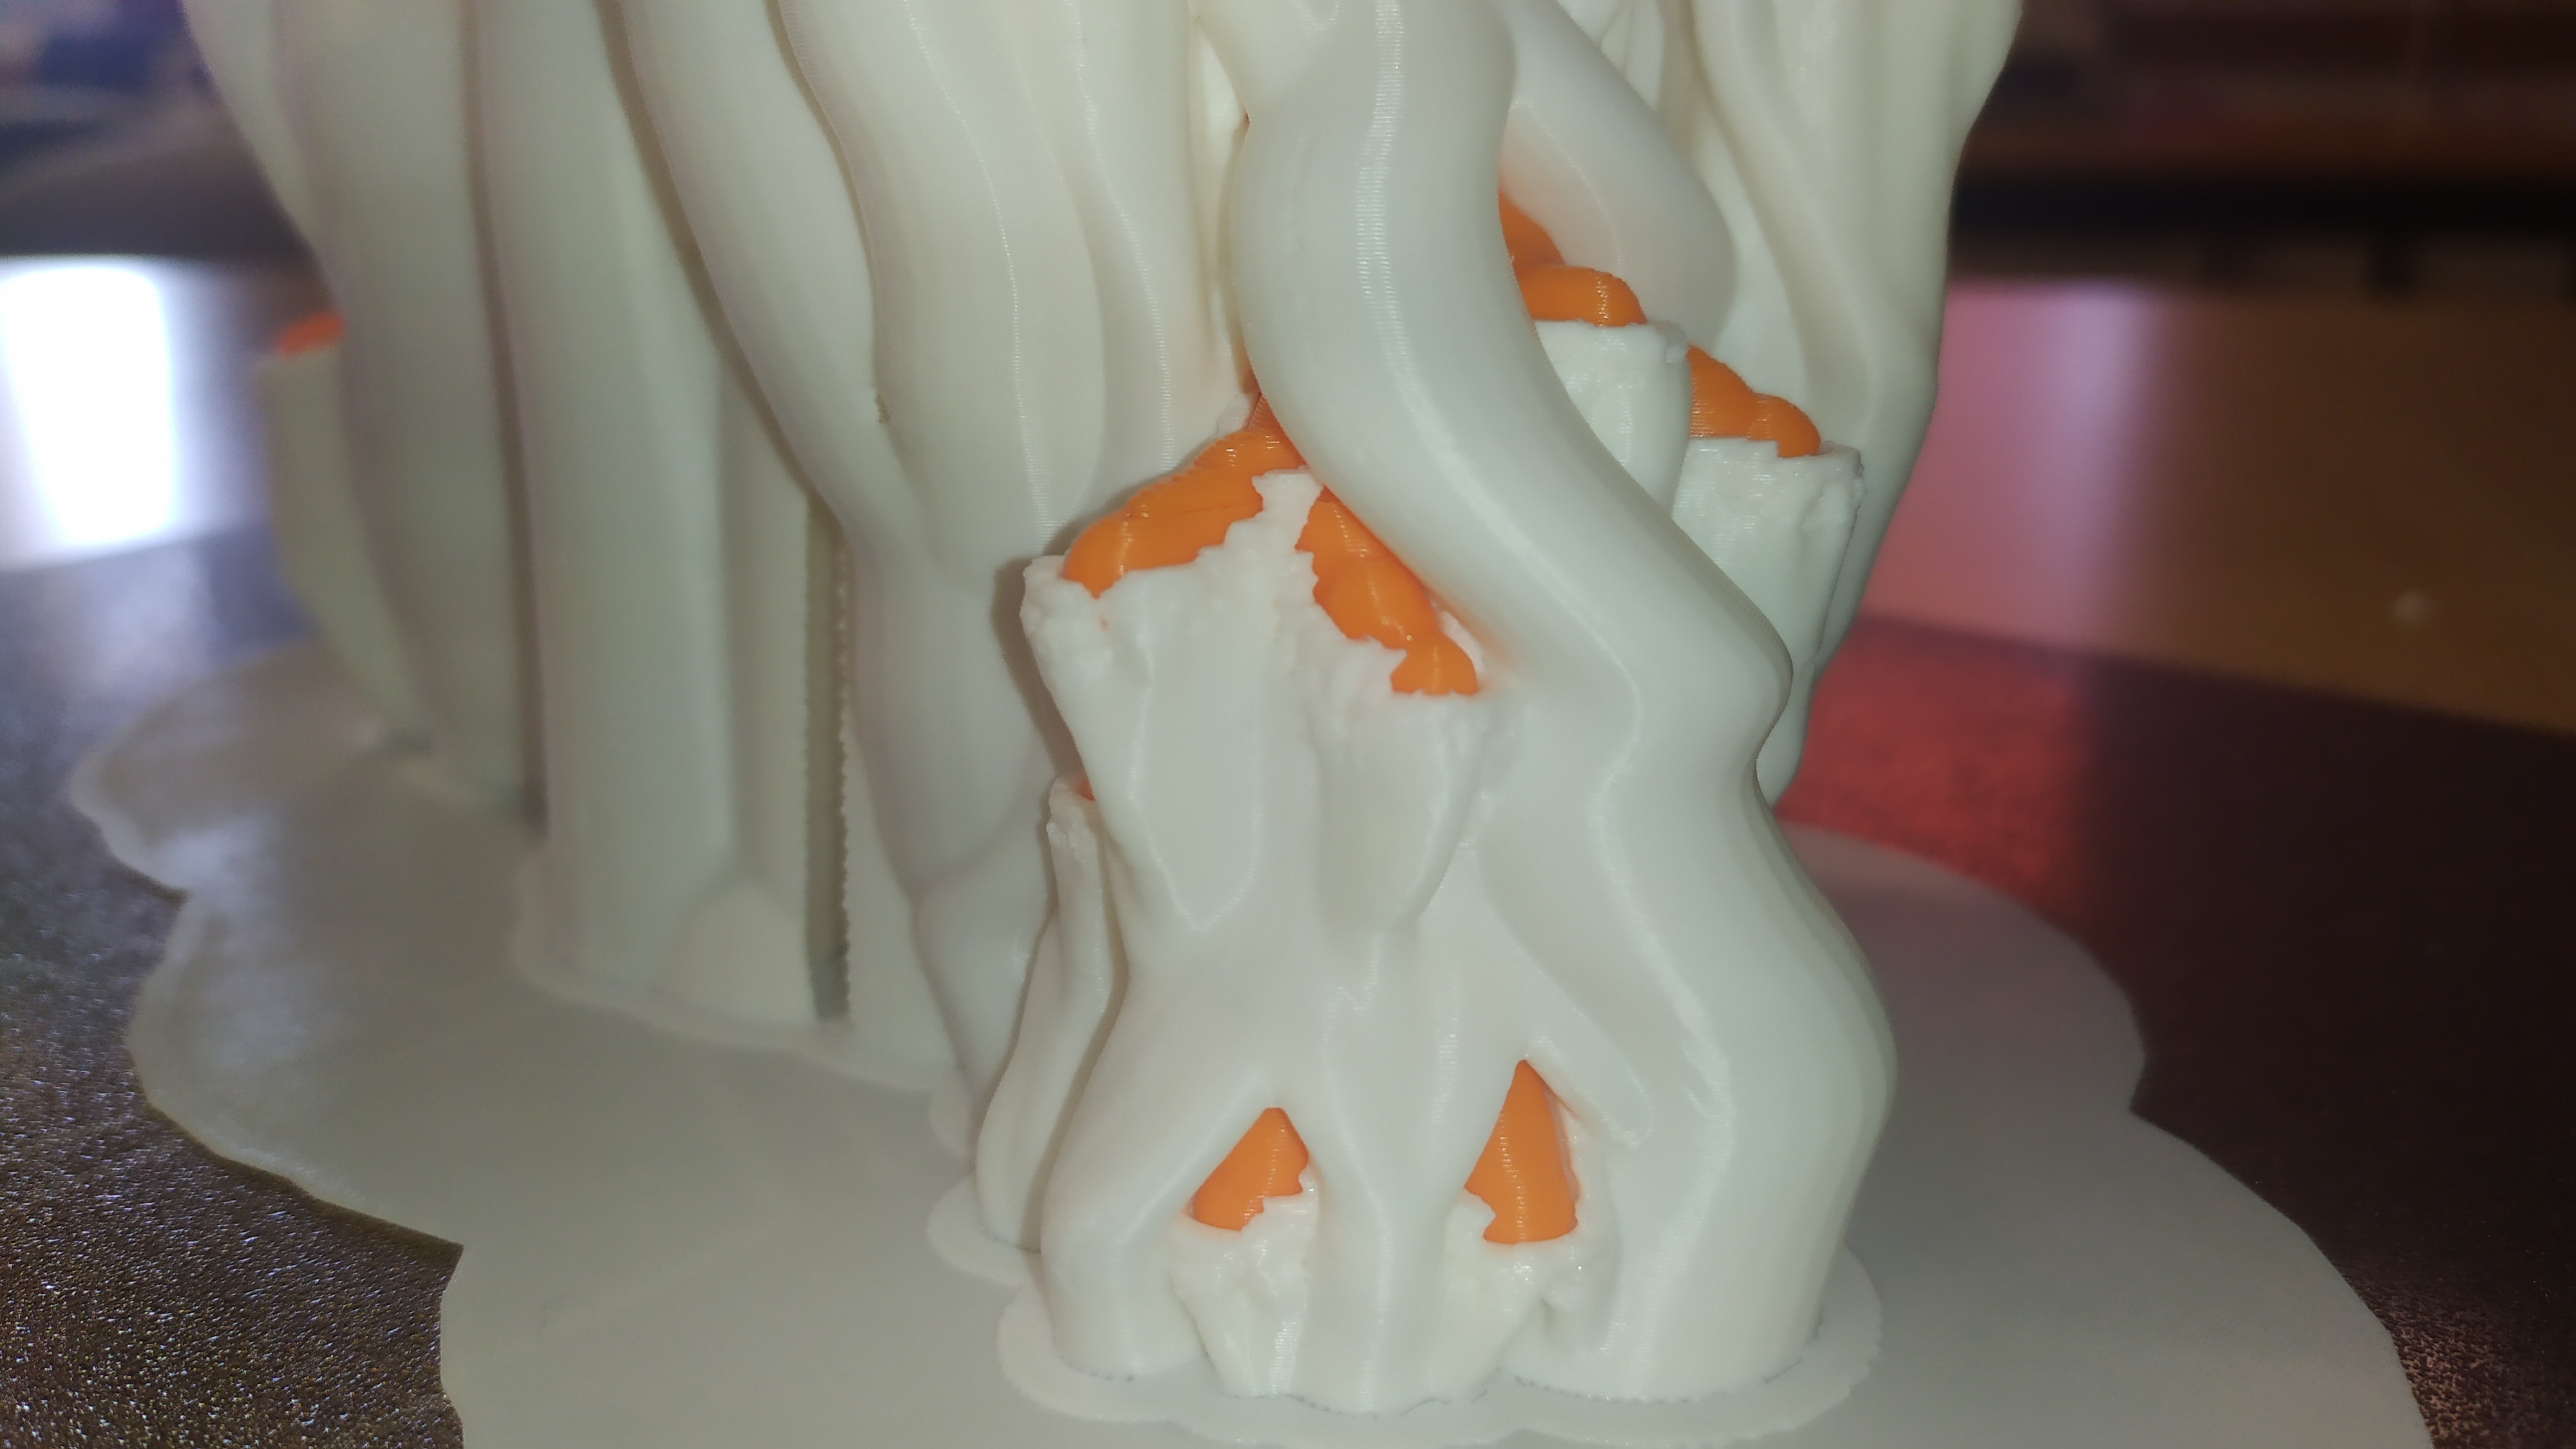
\includegraphics[width=0.72\textwidth]{fotos/impressao_inicial_pla.jpg}
  \caption{Testes de impressão da árvore brônquica com TPU 95A, com suporte em PLA.}
  \label{fig:impressao-inicial}
\end{figure}

A seleção de materiais foi considerada uma decisão crítica ao longo de todo o projeto, tendo sido identificados filamentos flexíveis como PEBA, TPU, TPE e TPC, filamentos especiais de dureza variável utilizados mais tarde no projeto e diferentes durezas comerciais, por exemplo 95A, 85A e 70A.
Como o objetivo do modelo era aproximar-se o mais possível da realidade anatómica, era necessário utilizar um material suficientemente mole, pelo que foi necessário testar vários materiais, geometrias e durezas ao longo do projeto.

\begin{figure}[htbp]
  \centering
  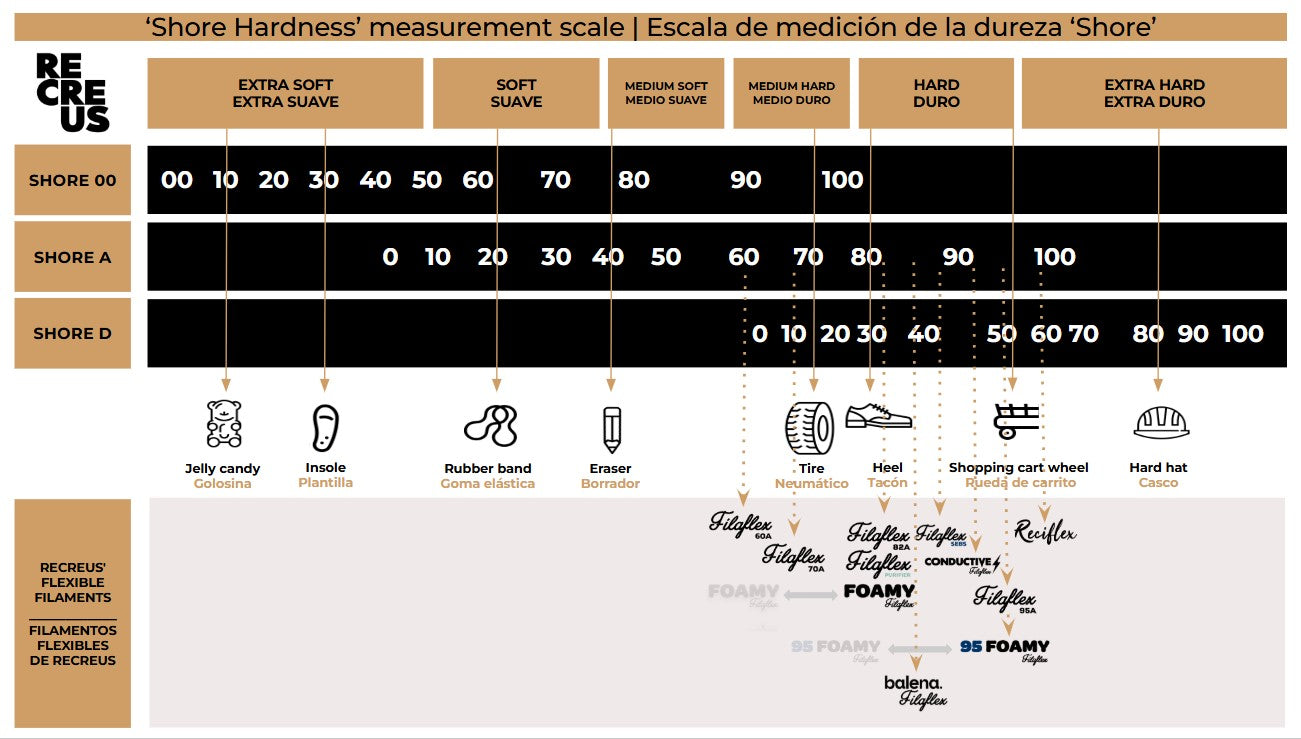
\includegraphics[width=0.9\textwidth]{fotos/shore_hardness_scale.jpg}
  \caption{Escala de dureza Shore aplicada a filamentos flexíveis, com exemplos de objetos do dia a dia em pontos equivalentes da escala (fonte: Recreus).}
  \label{fig:escala-shore}
\end{figure}

Nos filamentos maleáveis, quanto menor a dureza do material, mais difícil se torna a sua impressão. 
Os filamentos mais duros alimentam-se com facilidade através do extrusor, enquanto os mais moles tendem a comprimir-se e a deformar-se nas engrenagens de alimentação em vez de serem corretamente empurrados, o que aumenta significativamente a tendência para entupimentos e para defeitos de impressão, como o stringing. 
O TPU exige ainda um controlo mais apertado de vários parâmetros de impressão, nomeadamente a temperatura, que deve manter-se numa gama estreita, uma vez que poucos graus a mais podem ser o suficientes para provocar stringing ou distorções mais graves nas secções inclinadas por excesso de fluidez do material, a retração, que deve ser reduzida ao mínimo, já que retrações demasiado longas tendem a provocar entupimentos em vez de os evitar (devido á criação de stress entre a zona do estrusora e a secção de convecção que por sua vez faz com que o material se adere as paredes do bico e crie resistencia) e a velocidade de impressão, que deve ser mantida baixa, para permitir uma extrusão mais controlada. A dureza mais comum no mercado é a 95A, existindo ainda assim empresas que produzem filamentos especializados com durezas tão baixas como 85A ou mesmo 70A, sendo este último especialmente problemático, por se deformar com facilidade durante a impressão e por exigir um extrusor direct-drive dedicado para não encravar. Por esta razão, os testes iniciais foram realizados apenas com TPU 95A, com o objetivo de validar a viabilidade de impressão do modelo em materiais flexíveis, conforme documentado nos primeiros testes de impressão (\cref{fig:impressao-inicial}).

\subsection{Disposição do modelo para impressão}
\label{sec:disposicao-impressao}
Um outro desafio foi decidir como dispor o modelo para impressão em FDM, a única tecnologia disponível na universidade. Uma impressora SLA eliminaria alguns destes problemas de suporte, mas acabou por ser descartada, apesar de reunir mais vantagens do que a comparação inicial sugere:
\begin{itemize}
  \item Vantagens do SLA: dispensaria suportes em várias zonas do modelo, simplificando a geometria de impressão e reduzindo o risco de stringing no interior de peças ocas e ramificadas, um dos problemas que mais viria a afetar a impressão em FDM, como descrito mais adiante nesta secção. Permite também obter um acabamento de superfície muito mais fino e sem linhas de camada visíveis, característica relevante para reproduzir com fidelidade a superfície interna lisa da árvore brônquica. Além disso, existe atualmente uma grande variedade de resinas flexíveis e de silicones fotocuráveis compatíveis com esta tecnologia, com durezas Shore A que vão de aproximadamente 80A \parencite{FormlabsFlexible80A} até valores bastante mais baixos, como 70A \parencite{InslogicFlexible70A}, 63A ou 55A \parencite{LiqcreateFlexResins}, 50A \parencite{FormlabsElastic50A} ou mesmo 40A em resinas de silicone puro \parencite{FormlabsSilicone40A}, um intervalo mais alargado e mais fácil de alcançar de forma fiável do que o observado nos filamentos de FDM, em que durezas abaixo de 70A se tornam cada vez mais problemáticas de imprimir, precisamente porque o processo de cura de uma resina líquida não depende da extrusão mecânica de um filamento sólido através de engrenagens e de um bico;
  \item Desvantagens do SLA: equipamento com custo muito superior e dependente de equipamento adicional de pós-processamento, nomeadamente lavagem das peças em álcool isopropílico e cura adicional sob luz ultravioleta, o que tornava a sua aquisição incomportável para o projeto. Os volumes de impressão são também tipicamente mais reduzidos do que os disponíveis em impressoras FDM, o que poderia condicionar a impressão do modelo completo da árvore brônquica numa só peça.
\end{itemize}

Mantendo-se a impressão em FDM, foram equacionadas três opções para a disposição do modelo:
\begin{enumerate}
  \item \textbf{Impressão em peça única com suportes exteriores.} O modelo seria impresso de uma só vez, com suportes colocados do lado de fora para sustentar as zonas sem apoio inferior, que ficariam essencialmente a ser impressas ``no ar'':
  \begin{itemize}
    \item Vantagens: simplicidade de modificação da impressão e possibilidade de reaproveitar os próprios suportes como estrutura de fixação do modelo à base com os atuadores;
    \item Desvantagens: tempo de impressão elevado, uma vez que todo o modelo seria impresso de uma só vez, obrigando a reimprimir a peça inteira em caso de falha, com desperdício considerável de filamento, tempo e energia, além de os suportes só poderem ser colocados no exterior do modelo, deixando sem sustentação zonas interiores igualmente sujeitas a grandes deformações, sobretudo em materiais mais moles.
  \end{itemize}

  \item \textbf{Desdobramento e impressão individual das ramificações.} Esta opção passava por separar literalmente cada ramificação da malha num objeto independente e desdobrar a secção cilíndrica de cada ramo num plano, à semelhança do desdobramento de papel para construir um sólido, atribuindo-lhe espessura já na forma planificada e devolvendo-lhe a forma tridimensional apenas depois de impresso:
  \begin{itemize}
    \item Vantagens: possibilidade de modificar facilmente cada ramo de forma individual e de integrar sensores ou atuadores diretamente no modelo, caso necessário;
    \item Desvantagens: incerteza quanto à viabilidade do método, uma vez que, embora fosse possível desdobrar um ficheiro STL num plano com programas como o Blender, não havia garantia de que o mesmo funcionasse com um scan tão complexo e detalhado, podendo gerar erros ou geometrias inesperadas. A montagem após a impressão era também um risco, dado que os filamentos maleáveis são imprevisíveis e podem esticar ao serem retirados da base de impressão, criando folgas na união das peças e exigindo uma estratégia própria de costura entre secções, com uma probabilidade reduzida de sucesso ao longo de tantas ramificações.
  \end{itemize}

  \item \textbf{Moldagem por enchimento de um molde negativo.} Em vez de imprimir diretamente o modelo, esta opção previa a impressão de um molde negativo, utilizado depois para verter resina ou silicone e obter o positivo da árvore brônquica. Foi uma ideia forte durante grande parte do projeto, funcionando quase sempre como plano secundário:
  \begin{itemize}
    \item Vantagens: possibilidade de usar um material mais rígido no molde e um material extremamente mole no modelo positivo, bem como reutilizar o mesmo molde para produzir vários modelos sem o descartar;
    \item Desvantagens: como a árvore brônquica é oca, era necessário produzir um molde negativo tanto para a superfície exterior como para o espaço interior do modelo, ficando o positivo reduzido a uma película fina, com a espessura pretendida, encaixada entre esses dois moldes negativos. Isto obrigava a unir com precisão as três secções de molde em volta dessa película, o negativo interior e os dois lados do negativo exterior. A orientação das ramificações em várias direções dificultava ainda a remoção dos moldes sem danificar o modelo. Por fim, a geometria complexa e extensa não dava garantias de que fosse possível injetar resina ou silicone de forma uniforme em todos os cantos, com risco de inconsistências na espessura das paredes.
  \end{itemize}
\end{enumerate}

Mais tarde, motivadas pela futura aquisição de uma impressora Bambu Lab com dois bicos de impressão independentes (assunto detalhado mais adiante), foram ainda teorizadas duas variações aos métodos já descritos:
\begin{enumerate}
  \item \textbf{Suportes solúveis em PVA}, uma variação da impressão em peça única com suportes exteriores, substituindo o material dos suportes pelo filamento solúvel PVA:
  \begin{itemize}
    \item Vantagens: por ser solúvel em água, permitiria colocar suportes também no interior do modelo, em regiões críticas, aumentando a qualidade de impressão sem complicar o processo de remoção;
    \item Desvantagens: o PVA tem um custo por quilo superior ao do PLA e mesmo ao do TPU, já de si caro nas durezas mais baixas. Por ser sempre perdido após a dissolução em água, o custo de utilização tornar-se-ia incomportável. Esta variação acabou por nunca ser testada, por falta de tempo para adquirir o material.
  \end{itemize}

  \item \textbf{Molde negativo interno com imersão em resina}, uma variação do método dos moldes, recorrendo a uma resina especial de uso médico que solidifica em contacto com o ar, mantendo uma dureza específica de acordo com o tempo de exposição antes de a reação ser interrompida com um químico próprio. O processo consistiria em imprimir apenas o molde negativo interno da árvore brônquica, num material de fácil remoção como o PVA e mergulhá-lo repetidamente na resina, à semelhança do processo de fabrico de velas, sendo o número de imersões definido pela espessura pretendida para o modelo positivo. No final, bastaria dissolver o molde negativo em água:
  \begin{itemize}
    \item Vantagens: processo de produção muito simples;
    \item Desvantagens: o material do molde negativo tem um custo elevado, sendo sempre perdido no processo. Depois de impresso, o modelo, já sem qualquer rigidez estrutural própria, seria também difícil de fixar à estrutura de suporte dos manipuladores, exigindo peças de fixação dedicadas e de integração complexa.
  \end{itemize}
\end{enumerate}

Por estas razões, optou-se por manter o método de impressão em peça única com suportes exteriores.

\subsection{Evolução do processo de impressão 3D}
\label{subsec:evolucao-impressao}
Inicialmente, os suportes eram impressos no mesmo material do modelo, devido às limitações da maquinaria disponível na altura, com apenas um bico de impressão. Este método funcionava razoavelmente bem com filamentos de dureza elevada, como o 95A, mas mostrava-se bastante problemático com materiais mais moles, como o Filaflex TPE 70A. A mesma característica que tornava estes materiais interessantes para o projeto tornava-os também problemáticos. Ao usar o mesmo material para o suporte e para o objeto, toda a impressão se comportava como um único e grande objeto mole, cuja vibração aumentava com a altura já impressa, entrando em ressonância com o próprio movimento da cabeça de impressão e criando grandes inconsistências. Por frações de milissegundo e de milímetro, a posição da cabeça de impressão deixava de corresponder à posição real da última camada impressa. \hl{(vou adicionar imagens sobre isto nesta secção)}

Uma das soluções equacionadas para este problema passava por substituir o filamento por um material especial de dureza variável, com um agente expansivo interno que utiliza o próprio calor do bico como catalisador, permitindo teoricamente atingir durezas entre 80A e 50A consoante a temperatura, segundo a informação disponibilizada pela marca. O único inconveniente deste material seriam os resíduos gerados pelo agente expansivo, que poderiam comprometer a qualidade de impressão, ainda que de forma mitigável. Esta solução acabou por nunca ser necessária, pois, sensivelmente na mesma altura, a universidade adquiriu três novas impressoras 3D, entre elas uma Bambu Lab H2D, equipada com dois bicos independentes que permitem imprimir, em simultâneo, materiais com propriedades e compatibilidades distintas, uma aquisição que resolveu o problema.

Passou-se então a um método que mantinha o TPE 70A como material principal do modelo, mas com PLA como material de suporte, funcionando simultaneamente como suporte estrutural e como suporte de amortecimento de vibração para o modelo principal. \hl{(vou adicionar uma imagem sobre isto)}

Este método trouxe uma melhoria enorme na qualidade de impressão, mas tornou mais visíveis outros problemas. Como já referido, os materiais flexíveis de dureza muito baixa são especialmente difíceis de imprimir com fiabilidade. Este caso não foi exceção. Detetaram-se, durante e após a impressão, inconsistências de aderência entre camadas e entre paredes do objeto, camadas inteiras com falta de material, tornando-as propensas a quebrar ou rasgar e, o pior de todos os problemas, uma quantidade excessiva de stringing no interior do modelo, precisamente a zona mais importante para este trabalho. Isto persistia mesmo após inúmeras calibrações dos parâmetros de retração, da velocidade de impressão, da temperatura de impressão, do Pressure Advance e dos níveis de humidade do filamento. O Pressure Advance é uma funcionalidade do firmware do slicer que ajusta antecipadamente a pressão de extrusão nas mudanças de velocidade, reduzindo o babar de material e o stringing nos cantos. O TPU é, além disso, frequentemente descrito como uma ``esponja'', por ser um material higroscópico, ou seja, por absorver facilmente humidade do ar, sendo por isso necessário secá-lo constantemente e mantê-lo selado o máximo de tempo possível.

Foram também testadas técnicas e opções internas do slicer para mitigar o stringing, como alterar a localização da costura das paredes para uma zona menos visível, calibrar constantemente os valores de transição entre paredes, modificar as opções de geometria de retração e forçar as deslocações da cabeça de impressão a ocorrerem, sempre que possível, sobre as zonas de enchimento.

Ainda assim, nada resolvia de forma satisfatória o problema do stringing, nem mesmo técnicas de limpeza manual, como escovilhões para aquários, jatos de ar comprimido ou a queima das próprias linhas no interior do modelo. Algumas destas técnicas conseguiam reduzir a visibilidade do problema nas ramificações mais próximas da entrada, mas nas ramificações mais profundas era praticamente impossível.

A única forma de resolver, ou melhor, de mitigar este problema, foi escolher outro material como filamento flexível principal, o TPU MorPhlex 95A/75A, da empresa BiQU. Ao contrário dos outros filamentos de dureza variável considerados, apresenta uma transição de dureza fixa, começando com uma dureza de 95A antes de ser impresso e estabilizando permanentemente numa dureza de 75A\,$\pm$\,3A depois de impresso e aquecido. Esta caraterística torna-o muito mais estável, fiável e seguro do que as alternativas anteriores, permitindo, com a calibração correta, atingir uma qualidade de impressão quase perfeita e praticamente sem resíduos. Um outro ponto forte deste filamento é a sua cor, exclusiva da BiQU, muito próxima da cor real do interior do pulmão, o que o tornava ainda mais adequado a este trabalho.

Este material revelou, no entanto, uma deformação predominantemente plástica em vez de elástica quando sujeito a grandes esforços repetidos, como as contrações e expansões constantes que a atuação ativa das paredes exigiria, uma característica que viria a pesar mais tarde na avaliação da viabilidade de atuadores dedicados a essa deformação, discutida na \cref{sec:eletronica-alimentacao}.

\section{Seleção do sistema de atuação}
\label{sec:selecao-atuacao}
A definição do sistema de atuação foi uma das partes que mais evoluiu durante o projeto, sobretudo nas fases iniciais. A descrição dos movimentos pretendidos ainda não estava completamente consolidada e, por isso, foram exploradas soluções que mais tarde se revelaram pouco adequadas ao comportamento real que se pretendia reproduzir. Esta incerteza levou à análise de alternativas bastante diferentes entre si, desde motores de vibração, pensados para criar zonas de pressão localizada que pudessem sugerir o batimento cardíaco ou pequenas compressões das vias aéreas, até micro motores de passo, considerados para apertar gradualmente as paredes do modelo e simular constrangimentos associados ao ciclo respiratório.

Com a evolução do modelo da árvore brônquica e após a primeira reunião de acompanhamento com a equipa médica, tornou-se mais clara a natureza dos movimentos a implementar. O objetivo principal deixou de ser a criação de deformações locais independentes e passou a ser a reprodução controlada de deslocações globais e perturbações visíveis, associadas à respiração, ao batimento cardíaco e à tosse. Esta clarificação obrigou a rever a arquitetura de atuação inicialmente imaginada, baseada na distribuição de vários atuadores ao longo da árvore brônquica. Embora essa solução pudesse parecer direta para movimentos localizados, acabaria por tornar o sistema pesado do ponto de vista mecânico, aumentando o número de motores, exigindo uma estrutura de suporte muito próxima do modelo e introduzindo dificuldades adicionais de montagem, calibração, sincronização e manutenção.

A solução adotada passou, por isso, pela utilização de manipuladores robóticos capazes de posicionar uma plataforma móvel dentro de um volume de trabalho definido por coordenadas cartesianas. Nesta abordagem, o movimento deixa de depender de vários atuadores distribuídos pela árvore brônquica e passa a ser gerado a partir da trajetória imposta à plataforma. A complexidade é, assim, transferida para a descrição matemática do movimento, em particular para o cálculo da cinemática inversa, permitindo alterar perfis de respiração, batimento cardíaco ou tosse sobretudo por software, sem obrigar a modificar fisicamente a disposição dos motores.

Dentro desta lógica, foram estudadas diferentes configurações de manipuladores delta, uma vez que este tipo de robô paralelo utiliza vários braços ligados a uma plataforma móvel comum. Ao contrário de um manipulador serial, em que cada junta depende diretamente da anterior, num manipulador delta os braços trabalham em conjunto para posicionar a plataforma no espaço. Esta geometria permite obter movimentos rápidos, repetíveis e compactos, mantendo os atuadores fixos na base e reduzindo a massa em movimento. Para este projeto, estas características eram particularmente interessantes, pois permitiam atuar sobre a árvore brônquica sem instalar motores diretamente sobre o modelo.

Foram considerados dois tipos principais de solução. A primeira recorria a seis atuadores, dois por braço, permitindo controlar a translação da plataforma nos eixos \(X\), \(Y\) e \(Z\) e, adicionalmente, a sua orientação através de três graus de rotação. Esta configuração oferecia maior liberdade de movimento, mas introduzia uma complexidade mecânica e matemática superior à necessária para os fenómenos definidos para o protótipo. A segunda opção, posteriormente escolhida, utiliza apenas três atuadores, um por braço, controlando a posição da plataforma nos três eixos cartesianos. Apesar de não permitir comandar diretamente a rotação da plataforma, esta solução revelou-se suficiente para representar os deslocamentos pretendidos, simplificando a montagem, reduzindo o número de componentes e tornando mais direta a implementação da cinemática inversa.

Com esta decisão, a seleção dos atuadores passou a privilegiar servo-motores compactos, acessíveis e fáceis de controlar, tendo sido escolhidos os MG90S para a construção dos manipuladores. Esta escolha foi também reforçada pela comparação direta com motores de passo, avaliados em paralelo durante os testes iniciais de eletrónica. Apesar de os motores de passo garantirem maior capacidade de carga, a sua natureza de controlo em malha aberta obriga a uma rotina de homing sempre que o sistema é ligado, para que o motor recupere a noção da sua posição real, enquanto um servo-motor recebe apenas um comando de posição que pretende atingir (em formato de um sinal PWM) enviado num único sentido, cabendo ao seu controlador interno ajustar automaticamente, através de uma malha de controlo PID, o erro entre a posição atual e essa posição pretendida, até a atingir. Esta diferença simplifica significativamente o arranque e o funcionamento do sistema. A escolha destes servos foi ainda coerente com o objetivo de manter o sistema simples e repetível, concentrando a coordenação dos movimentos no firmware e no cálculo das posições da plataforma. Antes da montagem final, foram realizados testes de encaixe entre os MG90S e as peças impressas, verificando tolerâncias, alinhamento da patilha do servo e liberdade de rotação dos braços. Estes ensaios foram acompanhados por um processo gradual de calibração, no qual se confirmou a posição neutra de cada servo, os limites angulares admissíveis e a correspondência entre o comando PWM enviado pelo firmware e o movimento real observado no manipulador.

Esta escolha mecânica foi acompanhada, ainda numa fase inicial do projeto, pelo início do desenvolvimento do código de cinemática inversa associado a este tipo de manipulador, descrito em detalhe no capítulo 4.8. Ao longo deste processo, a validação do sistema foi feita de forma cruzada: o comportamento físico dos braços montados em bancada era comparado com as posições calculadas pelo firmware, permitindo ajustar limites, corrigir desvios e garantir que o movimento matematicamente previsto podia ser reproduzido de forma segura pela estrutura real.

\section{Eletrónica de controlo e alimentação}
\label{sec:eletronica-alimentacao}
O desenvolvimento da eletrónica teve início a meio do desenvolvimento do hardware, depois de confirmada a viabilidade de impressão do modelo e assim que os componentes eletrónicos chegaram, encontrando-se este passo diretamente ligado à implementação dos movimentos, uma vez que, sem eletrónica funcional, não era possível testar sensores, microcontroladores nem motores. A arquitetura prevista separa a interface de utilizador e o cálculo de alto nível do controlo direto dos atuadores, cabendo ao Raspberry Pi 4B a responsabilidade pela HMI, pela monitorização e pelo envio de comandos ou posições, enquanto o ESP32-S3 atua como microcontrolador de tempo real, recebendo dados por comunicação série e convertendo-os em comandos para os servos.

\begin{figure}[H]
  \centering
  \resizebox{\textwidth}{!}{%
  \begin{tikzpicture}[
    block/.style={draw, rounded corners=4pt, align=center, minimum width=2.8cm, minimum height=1.0cm, font=\small, thick},
    small/.style={draw, rounded corners=4pt, align=center, minimum width=1.8cm, minimum height=0.85cm, font=\small, thick},
    servo/.style={draw, rounded corners=4pt, align=center, minimum width=1.6cm, minimum height=0.85cm, font=\small, thick},
    group/.style={draw, dashed, rounded corners=5pt, inner sep=9pt},
    power/.style={-Latex, thick, red!75!black},
    serial/.style={Latex-Latex, thick, blue!70!black},
    pwm/.style={-Latex, thick, orange!85!black}
  ]
    \node[block, fill=gray!14] (fonte) {Fonte de\\Alimentação\\5\,V -- 10\,A};
    \node[block, left=2.5cm of fonte, fill=gray!10] (ups) {UPS/HAT\\Power\\Management};
    \node[block, left=2.5cm of ups, fill=blue!12] (pi) {Raspberry\\Pi 4B};
    \node[small, below=1.0cm of pi, xshift=-1.25cm, fill=green!12] (esp) {ESP32-S3};
    \node[small, below=1.0cm of pi, xshift=1.3cm, fill=gray!8] (monitor) {Monitor};

    \node[block, below=1.8cm of esp, xshift=-3.4cm, fill=orange!12] (drv1) {Driver 1};
    \node[servo, below=0.9cm of drv1, xshift=-1.7cm, fill=orange!7] (s1) {Servo\\Motor};
    \node[servo, below=0.9cm of drv1, fill=orange!7] (s2) {Servo\\Motor};
    \node[servo, below=0.9cm of drv1, xshift=1.7cm, fill=orange!7] (s3) {Servo\\Motor};

    \node[block, below=1.8cm of esp, xshift=3.6cm, fill=orange!12] (drv2) {Driver 2};
    \node[servo, below=0.9cm of drv2, xshift=-1.7cm, fill=orange!7] (s4) {Servo\\Motor};
    \node[servo, below=0.9cm of drv2, fill=orange!7] (s5) {Servo\\Motor};
    \node[servo, below=0.9cm of drv2, xshift=1.7cm, fill=orange!7] (s6) {Servo\\Motor};

    \node[group, fit=(drv1)(s1)(s2)(s3), label=below:{\small Manipulador Delta 1}] (delta1) {};
    \node[group, fit=(drv2)(s4)(s5)(s6), label=below:{\small Manipulador Delta 2}] (delta2) {};

    \draw[power] ($(fonte.north)+(0,0.75)$) -- node[right]{\small 230\,V CA} (fonte.north);
    \draw[power] (fonte) -- node[above]{\small 5\,V} (ups);
    \draw[power] (ups) -- node[above]{\small 5\,V} (pi);
    \draw[power] (pi.south west) to[bend right=18] node[left]{\small 5\,V} (esp.north);
    \draw[serial] (pi.south) to[bend left=10] node[right]{\small série} (esp.north east);
    \draw[power] (pi.south east) to[bend left=18] node[right]{\small 5\,V} (monitor.north);
    \draw[power] (ups.south) -- ++(0,-3.1) coordinate (dist5v) node[midway,right]{\small 5\,V};
    \draw[power] (dist5v) -| (drv1.north);
    \draw[power] (dist5v) -| (drv2.north);
    \draw[pwm] (esp) -- node[above left]{\small PWM} (drv1);
    \draw[pwm] (esp) -- node[above right]{\small PWM} (drv2);
    \draw[pwm] (drv1) -- (s1);
    \draw[pwm] (drv1) -- (s2);
    \draw[pwm] (drv1) -- (s3);
    \draw[pwm] (drv2) -- (s4);
    \draw[pwm] (drv2) -- (s5);
    \draw[pwm] (drv2) -- (s6);

    \node[draw, rounded corners=3pt, fill=white, align=left, inner sep=7pt,
          below=1.3cm of $(delta1.south)!0.5!(delta2.south)$, font=\small] {%
      \textcolor{red!75!black}{$\longrightarrow$}\;alimentação 5\,V\quad
      \textcolor{blue!70!black}{$\longleftrightarrow$}\;comunicação série\quad
      \textcolor{orange!85!black}{$\longrightarrow$}\;sinal PWM / comando%
    };
  \end{tikzpicture}}
  \caption{Esquema consolidado de alimentação, comunicação e comando dos dois manipuladores delta.}
  \label{fig:alimentacao-geral}
\end{figure}

\subsection{Testes iniciais de eletrónica}
Os primeiros testes de eletrónica focaram-se exclusivamente na validação individual de cada componente, antes de qualquer tentativa de integração. Começou por se confirmar uma alimentação estável e a comunicação com o ESP32, verificando se este arrancava corretamente e permitia programação, sendo nesta fase alimentado apenas pela porta série do computador, uma solução pensada como temporária mas que viria a manter-se, de forma incidental, durante grande parte do desenvolvimento. \hl{(vou adicionar aqui os esquemas elétricos de cada teste individual)}

Em seguida, testaram-se isoladamente os três tipos de atuadores considerados nesta fase, confirmando apenas que cada um podia ser ligado e posto em movimento. O motor de vibração foi ligado diretamente ao ESP32, por se esperar um consumo reduzido, enquanto o servo-motor e o micro motor de passo foram alimentados a partir de uma fonte externa regulável, com limite de corrente definido em \SI{2}{\ampere}. O servo foi testado a \SI{6}{\volt}, próximo do limite superior do intervalo de funcionamento especificado pelo fabricante para o MG90S, entre \SI{4.8}{\volt} e \SI{6}{\volt}, com o objetivo de obter uma velocidade de resposta favorável durante os testes de deformação localizada e concentrada das paredes do modelo, então ainda em avaliação. Já o motor de passo foi testado com um driver dedicado, alimentado a \SI{9}{\volt} a partir da mesma fonte regulável, cujo intervalo de saída ia dos \SI{3}{\volt} aos \SI{9}{\volt}.

\subsection{Arquitetura de alimentação e avaliação de motores de passo}
Foi por esta altura que se consolidou a escolha do manipulador delta e dos servo-motores como atuador principal, pelas razões detalhadas na \cref{sec:selecao-atuacao}, mantendo-se contudo, nesta fase do projeto, a hipótese de recorrer também a motores de passo para reproduzir movimentos de deformação e contração localizada das vias aéreas. Os esquemas iniciais de alimentação previam por isso dois níveis de tensão distintos. Um dos níveis destinava-se ao microcontrolador, aos servos e aos sensores, enquanto o outro seria dedicado exclusivamente aos motores de passo, tendo sido equacionadas duas arquiteturas possíveis para o obter:
\begin{itemize}
  \item Partir de uma fonte de \SI{12}{\volt}, alimentando diretamente os drivers dos motores de passo e reduzindo essa tensão através de um conversor step-down para os \SI{5}{\volt} do restante sistema;
  \item Partir de uma fonte de \SI{5}{\volt} e elevar a tensão através de conversores step-up dedicados aos drivers dos motores de passo, uma opção descartada devido ao consumo de potência e às perdas energéticas associadas a este tipo de conversão.
\end{itemize}
Por exclusão, a primeira arquitetura, baseada numa fonte de \SI{12}{\volt} e num conversor step-down, tornou-se a opção mais viável.

Foi também nesta fase que surgiu a decisão de acrescentar uma interface dedicada ao sistema, inicialmente pensada como um pequeno ecrã OLED mas rapidamente substituída pela solução final, um Raspberry Pi associado a um monitor integrado. Esta escolha trouxe consigo a necessidade de proteger o Raspberry Pi de perdas de alimentação inesperadas, um cuidado já conhecido de experiência anterior, uma vez que a perda de energia durante a escrita no cartão SD onde reside o sistema operativo pode corromper esse cartão ou, em casos mais graves, danificá-lo de forma permanente. Como o Raspberry Pi é tipicamente alimentado através de uma porta de \SI{5}{\volt} e \SI{3}{\ampere}, esta necessidade era compatível com a arquitetura de \SI{12}{\volt} e conversor step-down já equacionada para os motores de passo.

\subsection{Dimensionamento da fonte de alimentação}
O dimensionamento da fonte teve por base o cenário então previsto de três manipuladores delta, correspondendo a nove servos MG90S. Este servo apresenta um consumo nominal entre 150 e \SI{250}{\milli\ampere}, mas pode atingir cerca de \SI{700}{\milli\ampere} em condição de bloqueio (stall), pelo que, ainda que fosse pouco provável que todos os nove servos entrassem em stall em simultâneo, se optou por dimensionar sempre para o pior caso possível, de forma a garantir o funcionamento do sistema mesmo nas condições mais exigentes, resultando este valor de bloqueio numa corrente total próxima dos \SI{6.3}{\ampere} para os nove servos, contra apenas \SI{2.6}{\ampere} em regime nominal. Os motores de passo, por sua vez, foram teorizados num total de seis unidades distribuídas pelo modelo, cada uma com um consumo máximo de \SI{150}{\milli\ampere}, o que acrescentava cerca de \SI{900}{\milli\ampere} ao total. Somando ainda o consumo do Raspberry Pi, estimado em \SI{3}{\ampere}, o cenário de \SI{12}{\volt} resultava numa corrente total próxima dos \SI{10.5}{\ampere}, sendo expectável que, com recurso a um conversor step-down, a corrente efetivamente exigida à fonte pelos servos e pelo Raspberry Pi fosse consideravelmente menor do que este valor calculado diretamente a \SI{5}{\volt}.

Esta arquitetura acabou, no entanto, por não avançar. Após várias discussões, concluiu-se que a utilização de motores de passo para reproduzir contrações e dilatações localizadas das vias aéreas seria uma implementação de elevada complexidade, sobretudo devido ao comportamento do filamento MorPhlex então em uso, que revelava uma deformação predominantemente plástica em vez de elástica sob grandes esforços repetidos, como as contrações e expansões constantes que este tipo de atuação exigiria, conforme já referido na \cref{subsec:evolucao-impressao}. Com a exclusão dos motores de passo, deixou de haver justificação para manter os dois níveis de tensão e para a fonte de \SI{12}{\volt}, tendo o sistema sido simplificado para um único nível de \SI{5}{\volt}, com uma corrente total estimada, para o pior caso possível, de cerca de \SI{9.6}{\ampere}. Foi por isso escolhida uma fonte de alimentação de \SI{5}{\volt} e \SI{10}{\ampere}, com margem suficiente acima do valor estimado.

Com a fonte selecionada, foram realizados testes com os dois manipuladores a funcionar em simultâneo, tendo-se observado uma pequena variação de tensão, entre 100 e \SI{200}{\milli\volt}, associada aos picos de corrente na comutação dos servos. Ainda que este valor não pareça elevado, procurou-se minimizá-lo ao máximo, uma vez que o Raspberry Pi é particularmente sensível a variações na sua alimentação, podendo sofrer reinícios inesperados mesmo com uma placa UPS a atuar como filtro adicional contra este tipo de perturbação. A pesquisa realizada confirmou ser prática comum a colocação de condensadores de desacoplamento junto à alimentação de cada servo, para atenuar precisamente este tipo de queda de tensão transitória, com a documentação e os fóruns consultados a recomendarem valores tipicamente entre os 230 e os \SI{700}{\micro\farad}. Optou-se por condensadores de \SI{470}{\micro\farad} junto de cada servo. \hl{(vou adicionar imagens sobre isto)}

\subsection{Gestão de energia do Raspberry Pi}
Mais tarde, o projeto passou de três para apenas dois manipuladores delta, reduzindo a complexidade face aos resultados pretendidos e diminuindo ainda mais a carga total sobre a fonte de alimentação. Em contrapartida, foi selecionada a UPS/HAT Suptronics X1209, que dispõe de duas entradas de alimentação distintas, uma de \SI{5}{\volt} e \SI{5}{\ampere} e outra entre os \SI{6}{\volt} e os \SI{18}{\volt} até \SI{3}{\ampere}, uma flexibilidade que permitiu continuar a utilizar a mesma fonte de \SI{5}{\volt} e \SI{10}{\ampere} já escolhida anteriormente. Ao contrário de grande parte das alternativas pesquisadas, que ou se limitavam a placas de gestão de energia bastante dispendiosas, ou eram placas de bateria incapazes de assegurar uma transição fiável entre a alimentação de rede e a alimentação por bateria, por serem pensadas apenas para funcionar a partir da bateria, esta HAT combina simultaneamente as funções de UPS e de gestão de energia, o que justificou a sua escolha. Foi associada a uma bateria LiPo de \SI{2100}{\milli\ampere\hour} e \SI{3.7}{\volt}.

\subsection{Da protoboard à PCB}
Depois de concluídos os testes do circuito numa protoboard, o mesmo foi transferido para uma PCB pré-furada, onde foram implementados os drivers referidos anteriormente, um por cada manipulador delta, cada um responsável por controlar os três servos correspondentes. Foi também montada e soldada uma PCB própria para alojar o microcontrolador ESP32-S3. Cada driver recebe os comandos enviados pelo ESP32 e a alimentação diretamente da fonte principal, distribuída através de um barramento comum a cada um dos três servos, sempre por intermédio do respetivo condensador de desacoplamento. O ESP32, por sua vez, pode ser alimentado pelo Raspberry Pi através de USB-C, mantendo simultaneamente a ligação série necessária à comunicação.

A lista completa dos componentes principais previstos para o sistema encontra-se na \cref{tab:componentes-hardware}, no Apêndice.

\section{Integração mecânica}
\label{sec:integracao-mecanica}
A integração mecânica deve garantir que o movimento é transmitido à árvore brônquica sem esforços excessivos, folgas significativas ou interferência com a passagem do broncoscópio, permitindo ainda um acesso fácil para manutenção, limpeza e substituição de peças. Para proteger o modelo e os atuadores, os limites de curso do manipulador e os limites angulares dos servos são definidos diretamente no firmware, evitando posições impossíveis ou capazes de danificar o modelo.

A estrutura de suporte do modelo passou por várias iterações ao longo do projeto, evoluindo de soluções simples e estáticas, pensadas apenas como apoio temporário para os primeiros testes, até uma estrutura única e mais complexa, capaz de alojar os dois manipuladores delta, as PCBs de controlo e o próprio modelo impresso da árvore brônquica, permitindo uma montagem simples e compacta de todo o sistema. Nas primeiras fases, cada manipulador foi montado sobre uma base independente, sem qualquer ligação entre si, servindo apenas para validar isoladamente a montagem mecânica e o funcionamento elétrico básico de cada braço (\cref{fig:suporte-estrutura-simples}). Esta abordagem, ainda que suficiente para os primeiros testes, tornava a integração posterior mais trabalhosa, obrigando a ligar e a posicionar manualmente cada manipulador sempre que se pretendia testar o conjunto.

\begin{figure}[htbp]
  \centering
  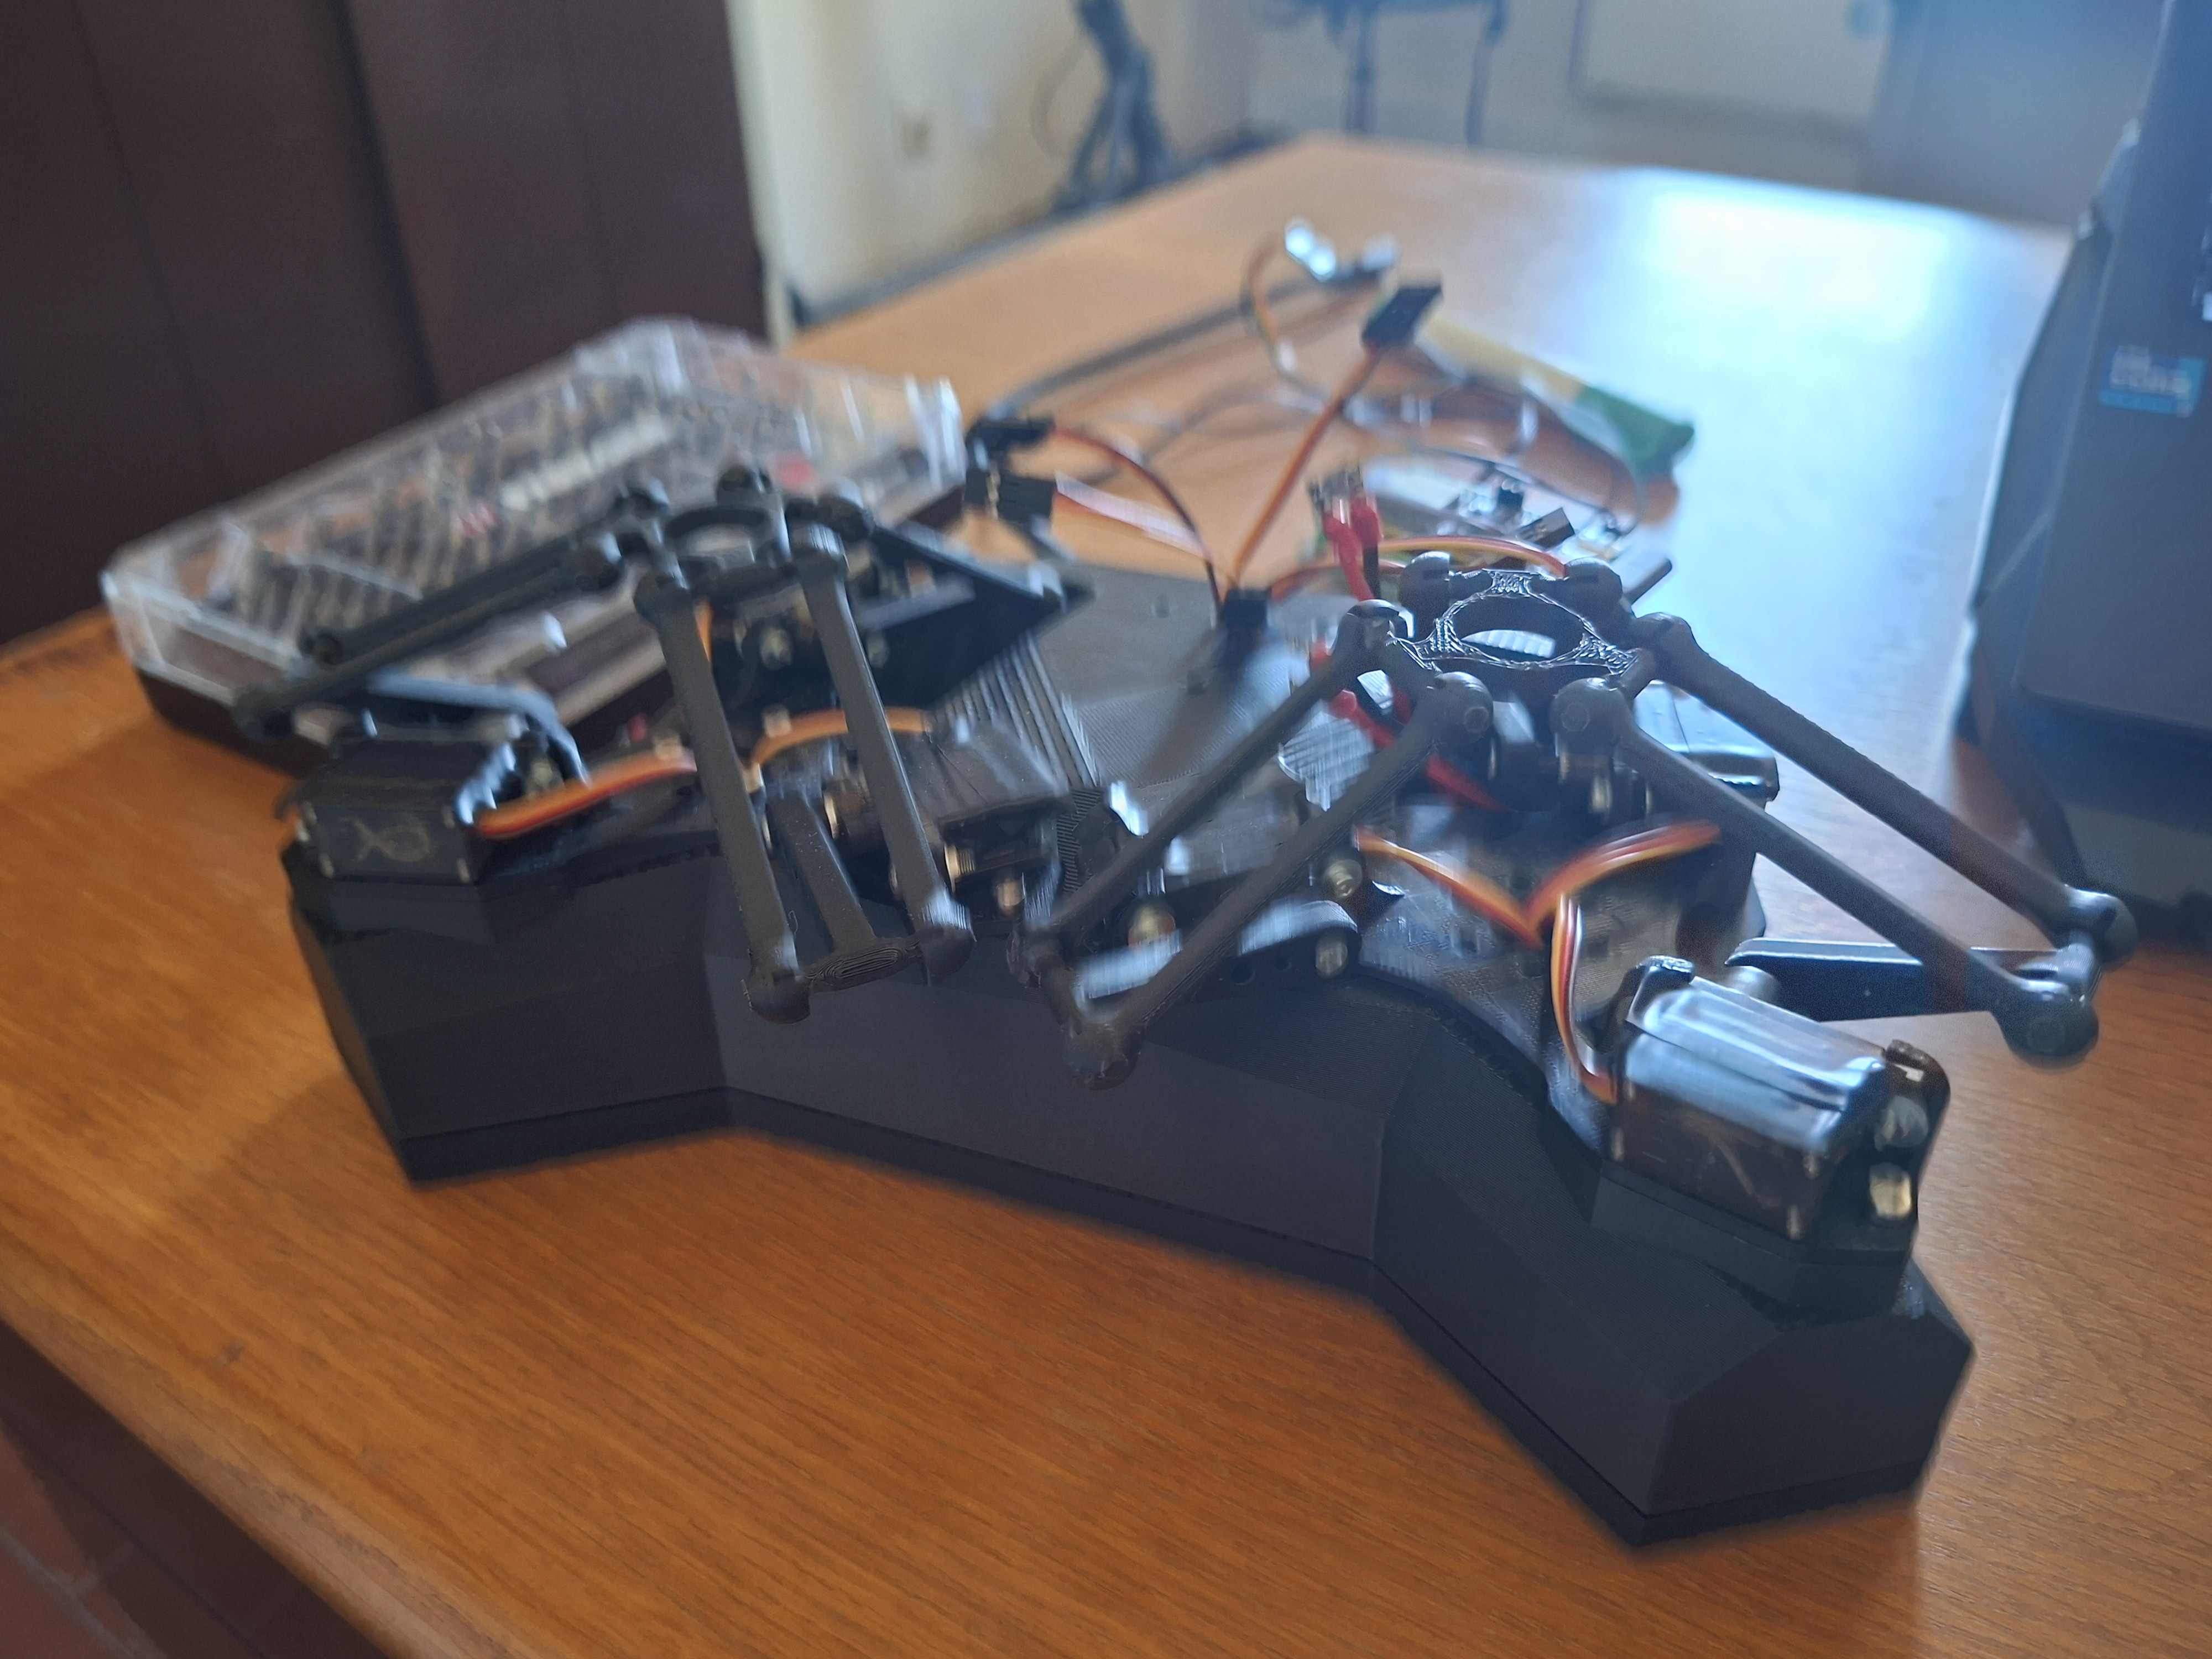
\includegraphics[width=0.72\textwidth]{fotos/suporte_estrutura_simples.jpg}
  \caption{Primeira iteração da estrutura de suporte, com cada manipulador delta assente sobre uma base independente, sem integração entre si.}
  \label{fig:suporte-estrutura-simples}
\end{figure}

A estrutura final resolveu esta limitação ao unificar os dois manipuladores numa única peça impressa, com encaixes dedicados para as PCBs dos drivers e pontos de fixação para o modelo da árvore brônquica, tal como ilustrado na \cref{fig:suporte-estrutura-integrada}. Esta solução reduziu significativamente o tempo de montagem e desmontagem do sistema completo, além de manter fixa a posição relativa entre os dois manipuladores, um requisito importante para a repetibilidade dos movimentos representados no modelo.

\begin{figure}[htbp]
  \centering
  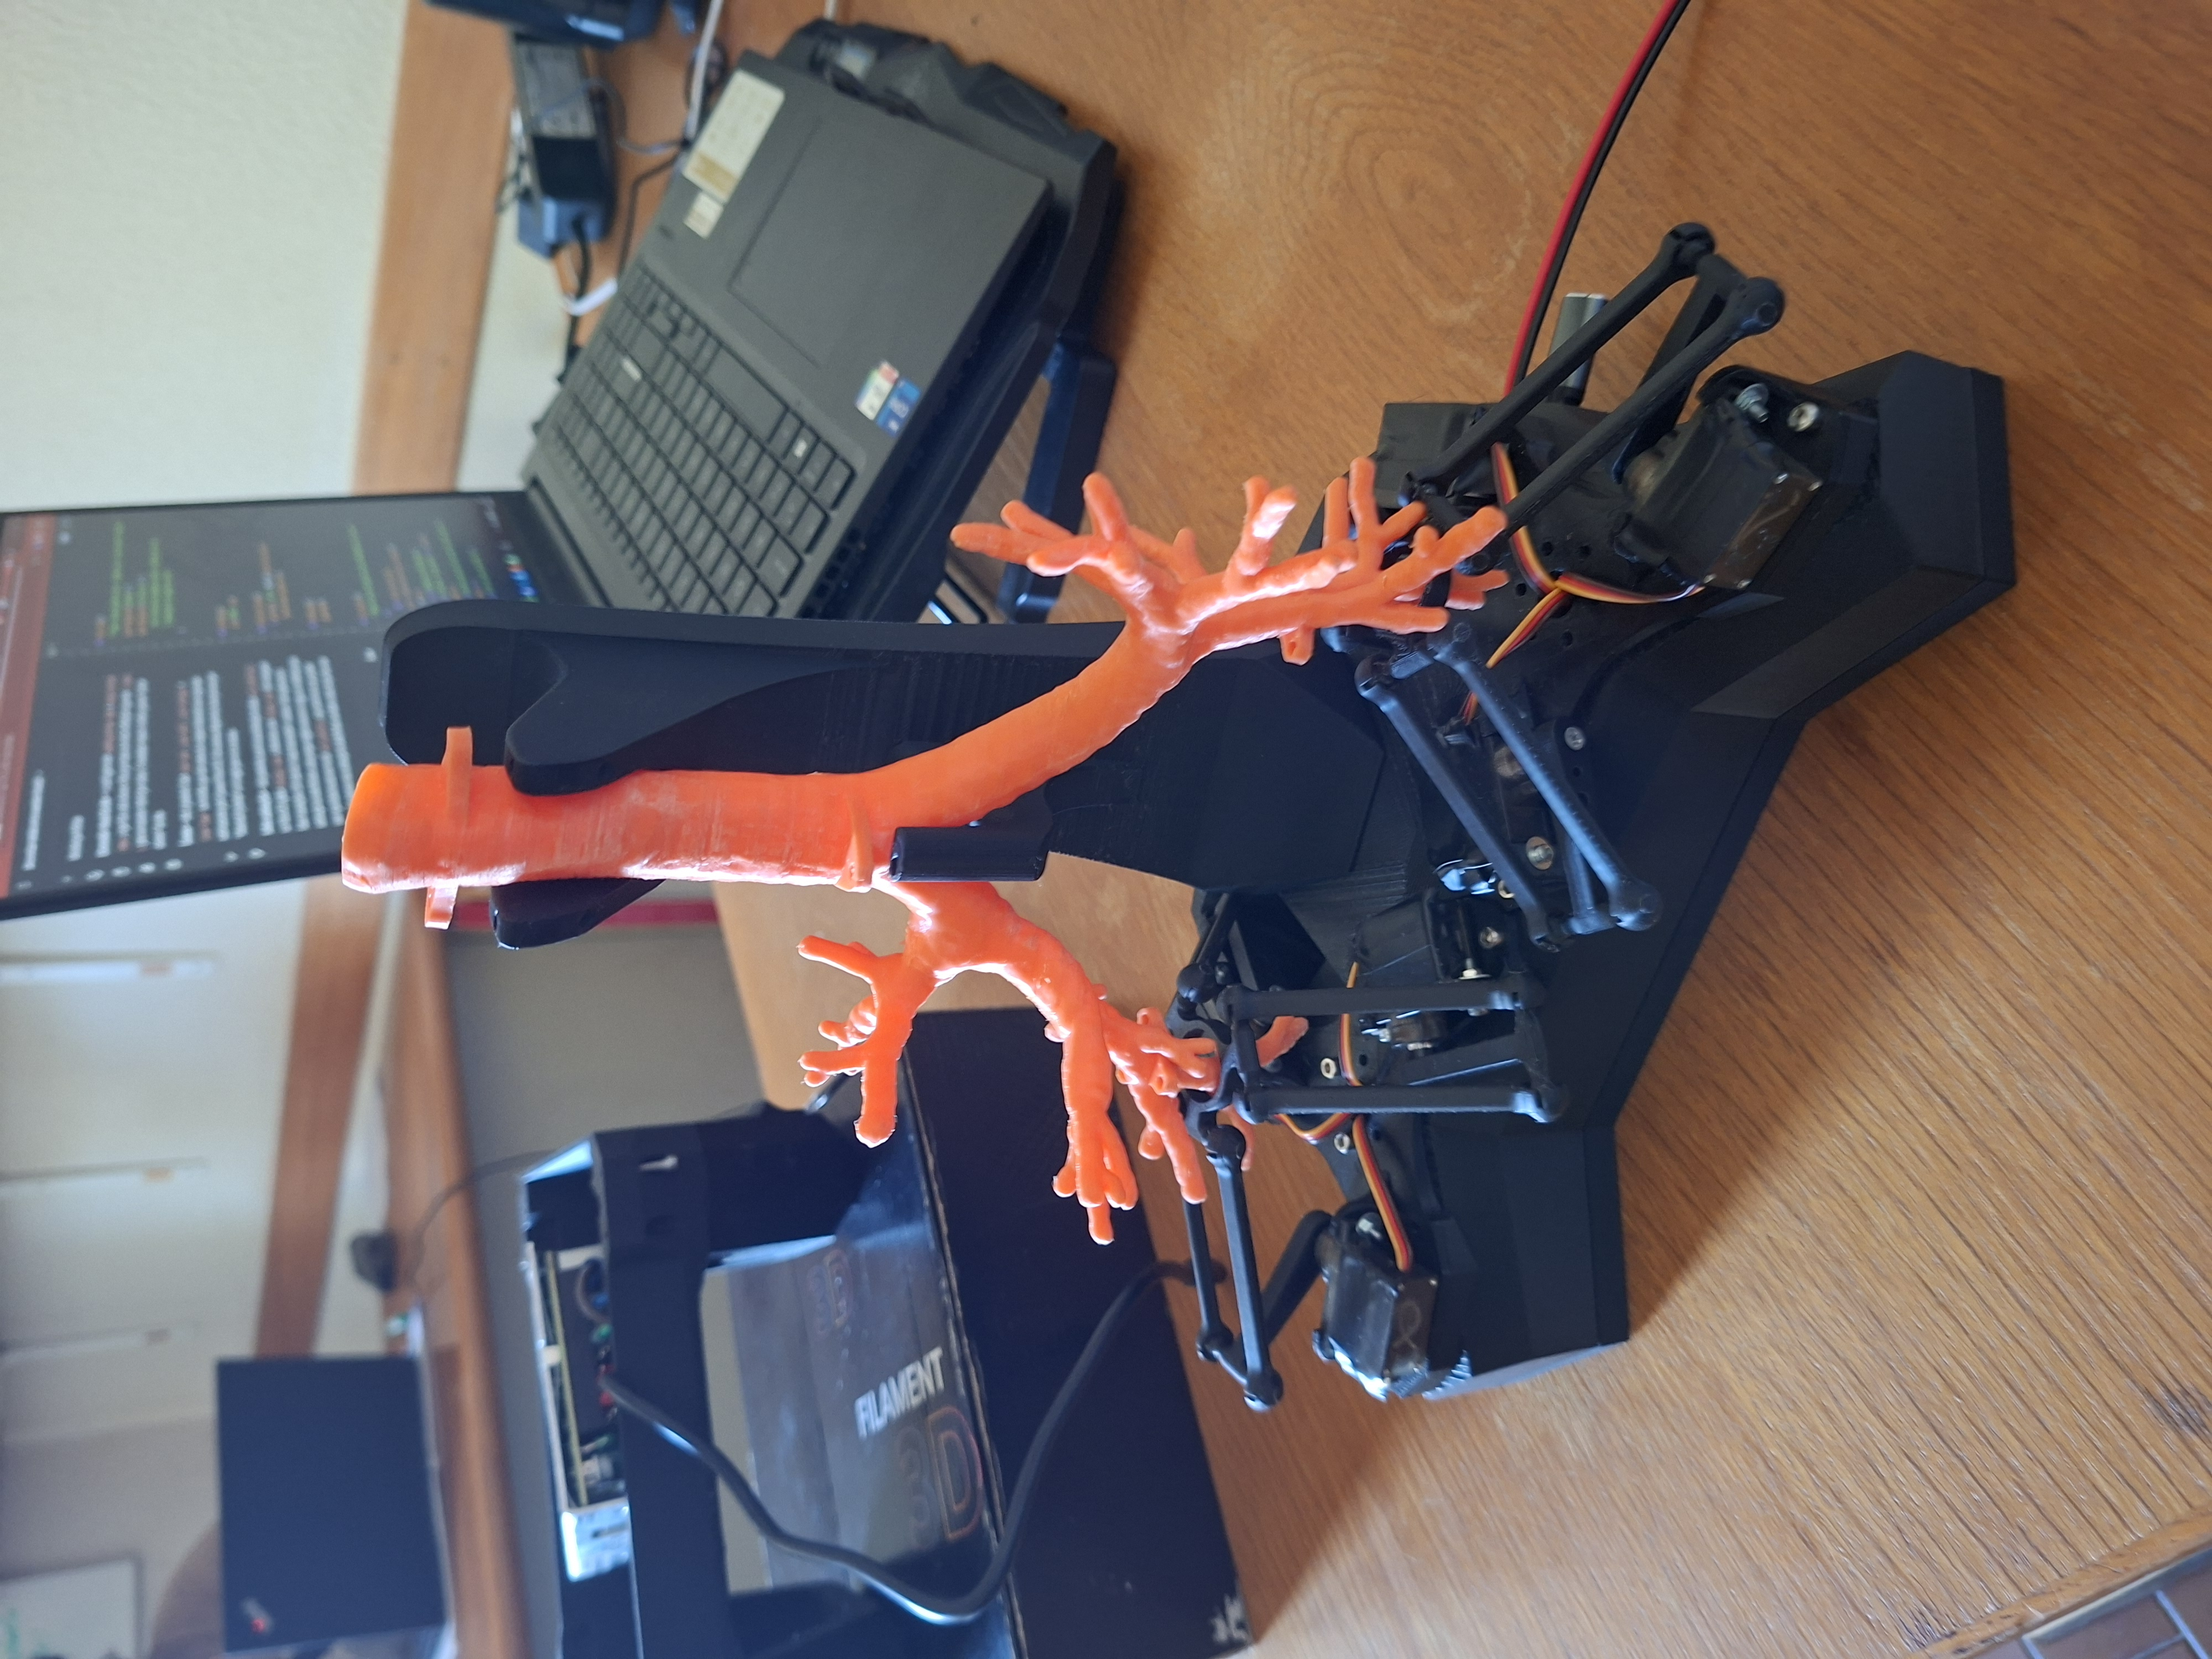
\includegraphics[width=0.72\textwidth]{fotos/suporte_estrutura_integrada.jpg}
  \caption{Estrutura de suporte final, integrando os dois manipuladores delta, os encaixes para as PCBs de controlo e os pontos de fixação do modelo da árvore brônquica numa única peça impressa.}
  \label{fig:suporte-estrutura-integrada}
\end{figure}

A fase de montagem começou pela impressão das peças estruturais em PLA preto, incluindo a base circular, os braços superiores, os elos de ligação e a plataforma móvel central. Numa primeira fase, a estrutura foi montada sem servos para verificar folgas, alinhamento das articulações e comportamento geométrico do conjunto (\cref{fig:delta-estrutura-mecanica}), etapa que permitiu identificar zonas onde era necessário rever tolerâncias e confirmar que os braços articulados rodavam sem bloqueio.

\begin{figure}[htbp]
  \centering
  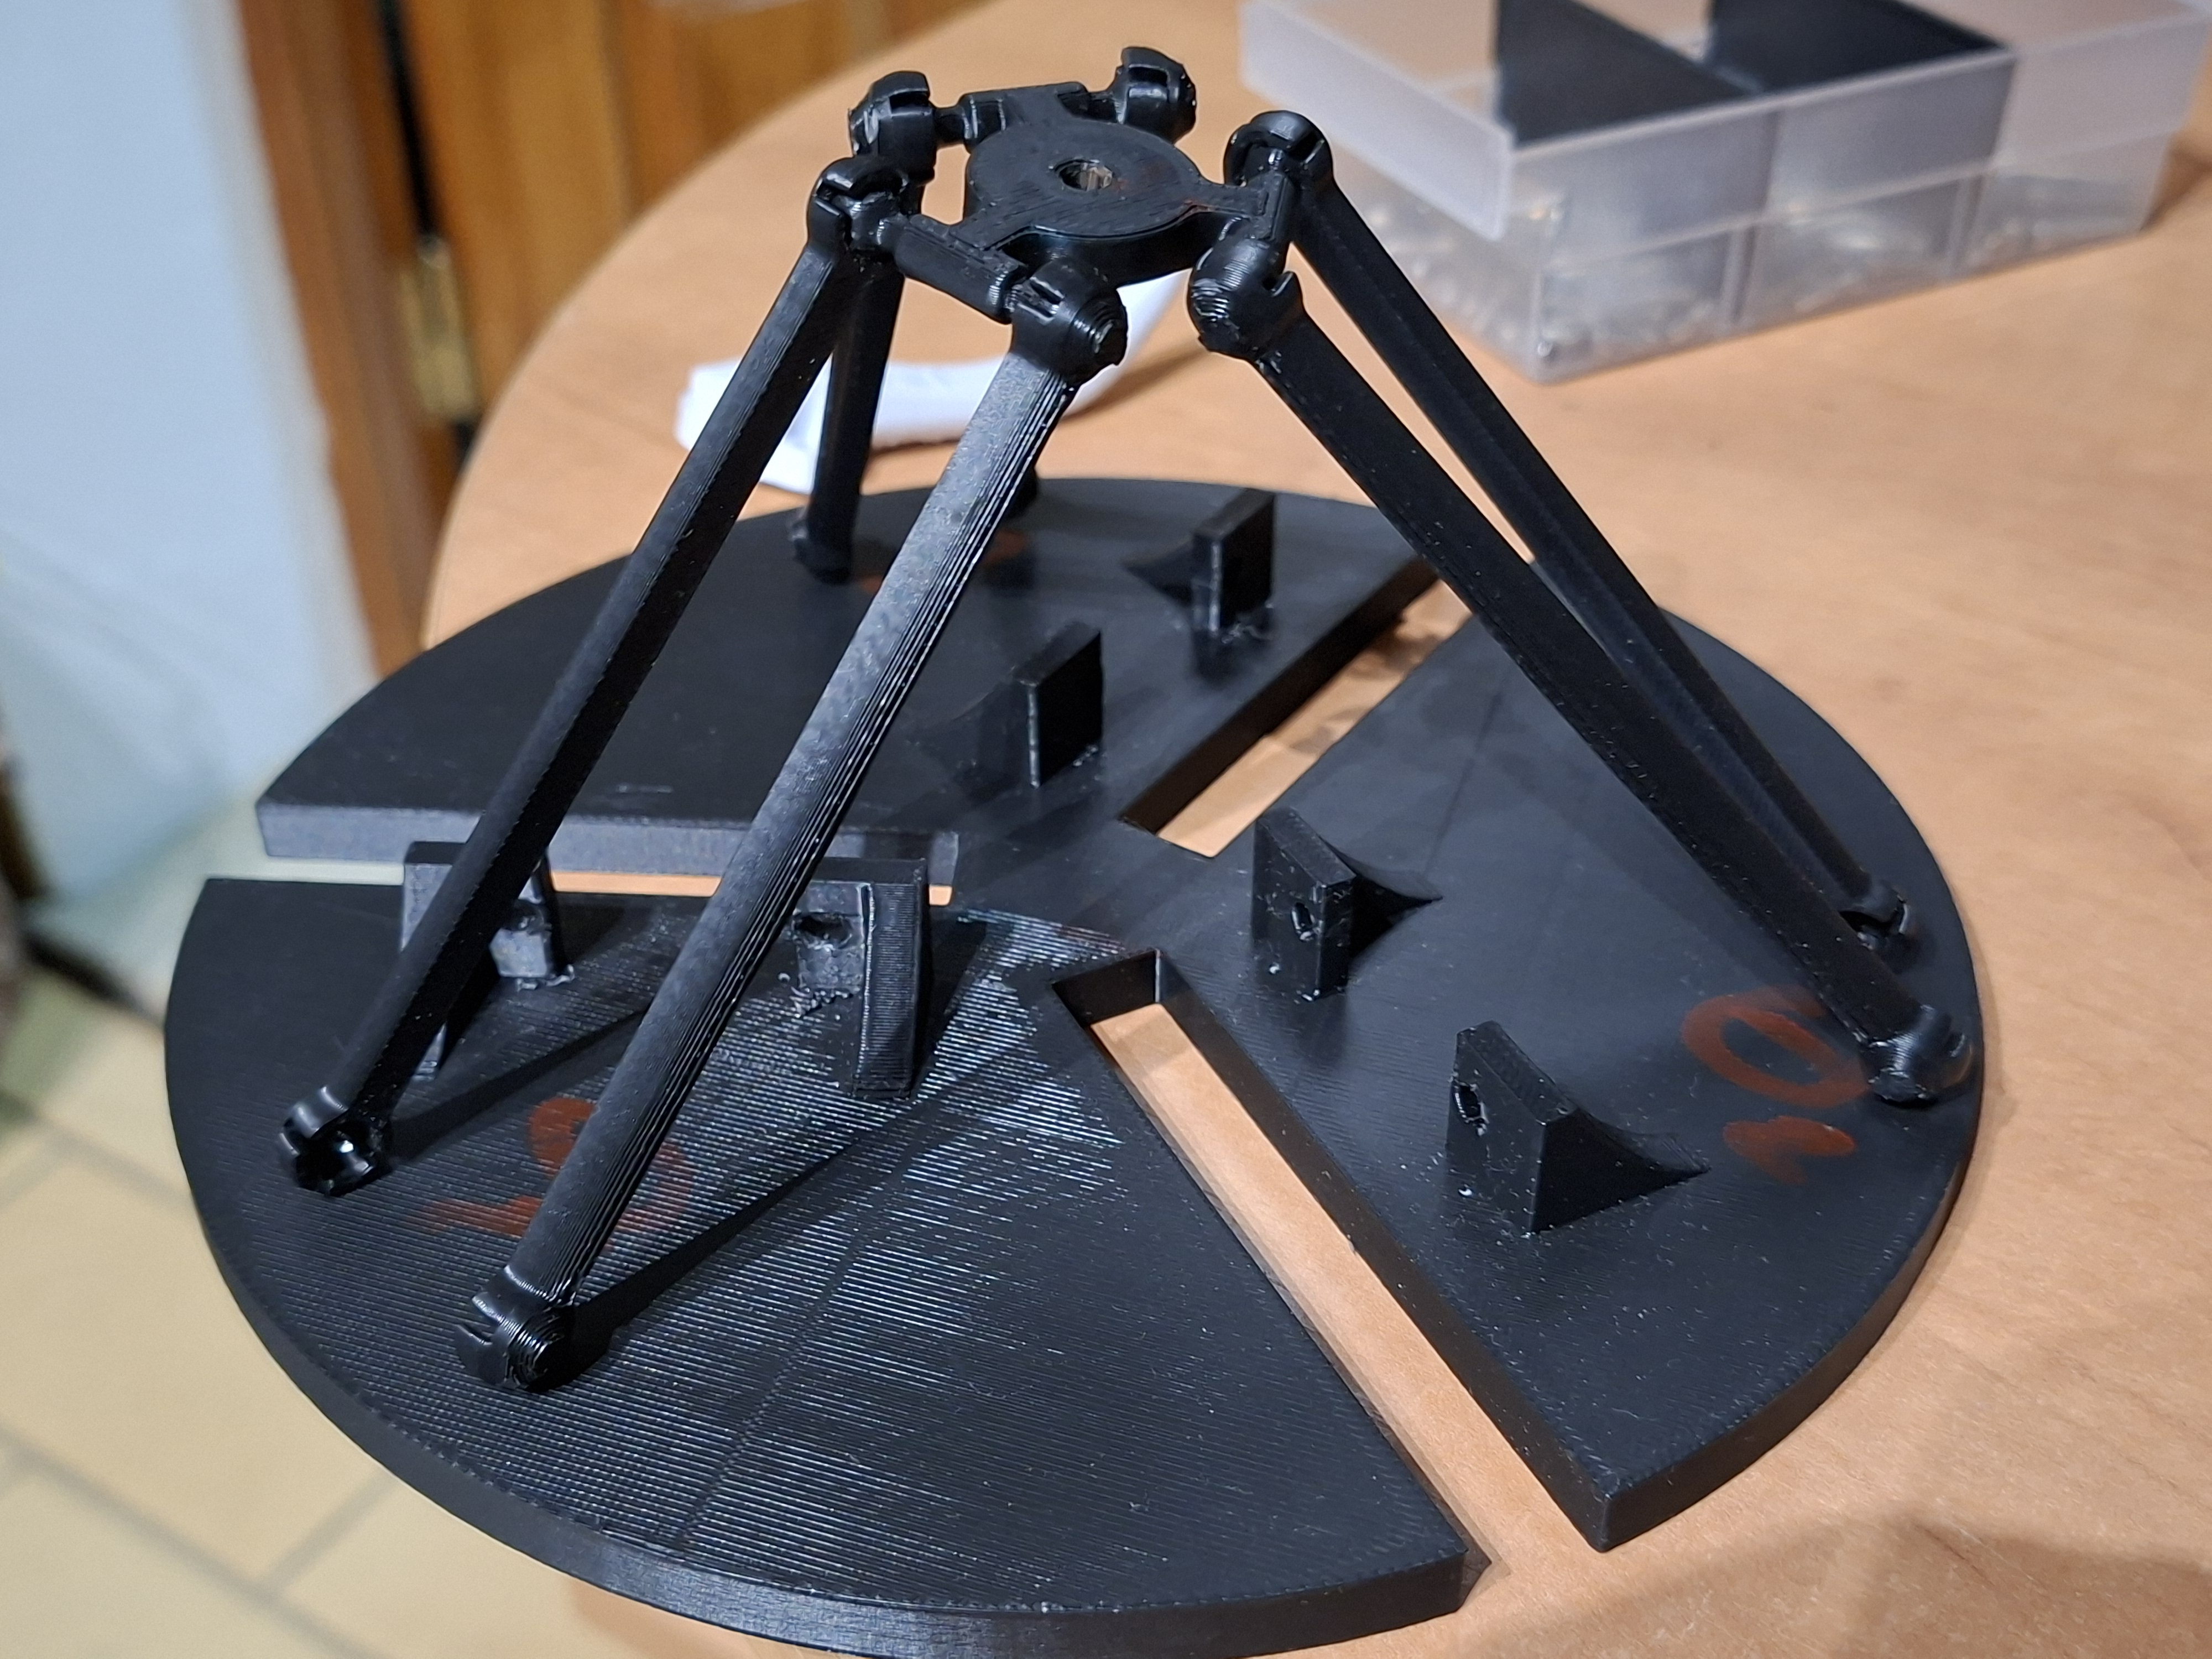
\includegraphics[width=0.72\textwidth]{fotos/delta_estrutura_mecanica.jpg}
  \caption{Estrutura mecânica de um manipulador delta em PLA preto, antes da instalação dos servos. A base circular e os três braços articulados estão já montados.}
  \label{fig:delta-estrutura-mecanica}
\end{figure}

A instalação dos servos foi feita de forma gradual, com validação individual de cada canal, tendo os dois manipuladores sido testados, numa fase intermédia, com ligações diretas ao ESP32 sem PCB de interface, usando jumpers para confirmar o funcionamento elétrico básico antes de qualquer ligação definitiva. A \cref{fig:delta-dois-manipuladores} mostra os dois manipuladores montados com todos os servos instalados, prontos para a fase de calibração de firmware.

\begin{figure}[htbp]
  \centering
  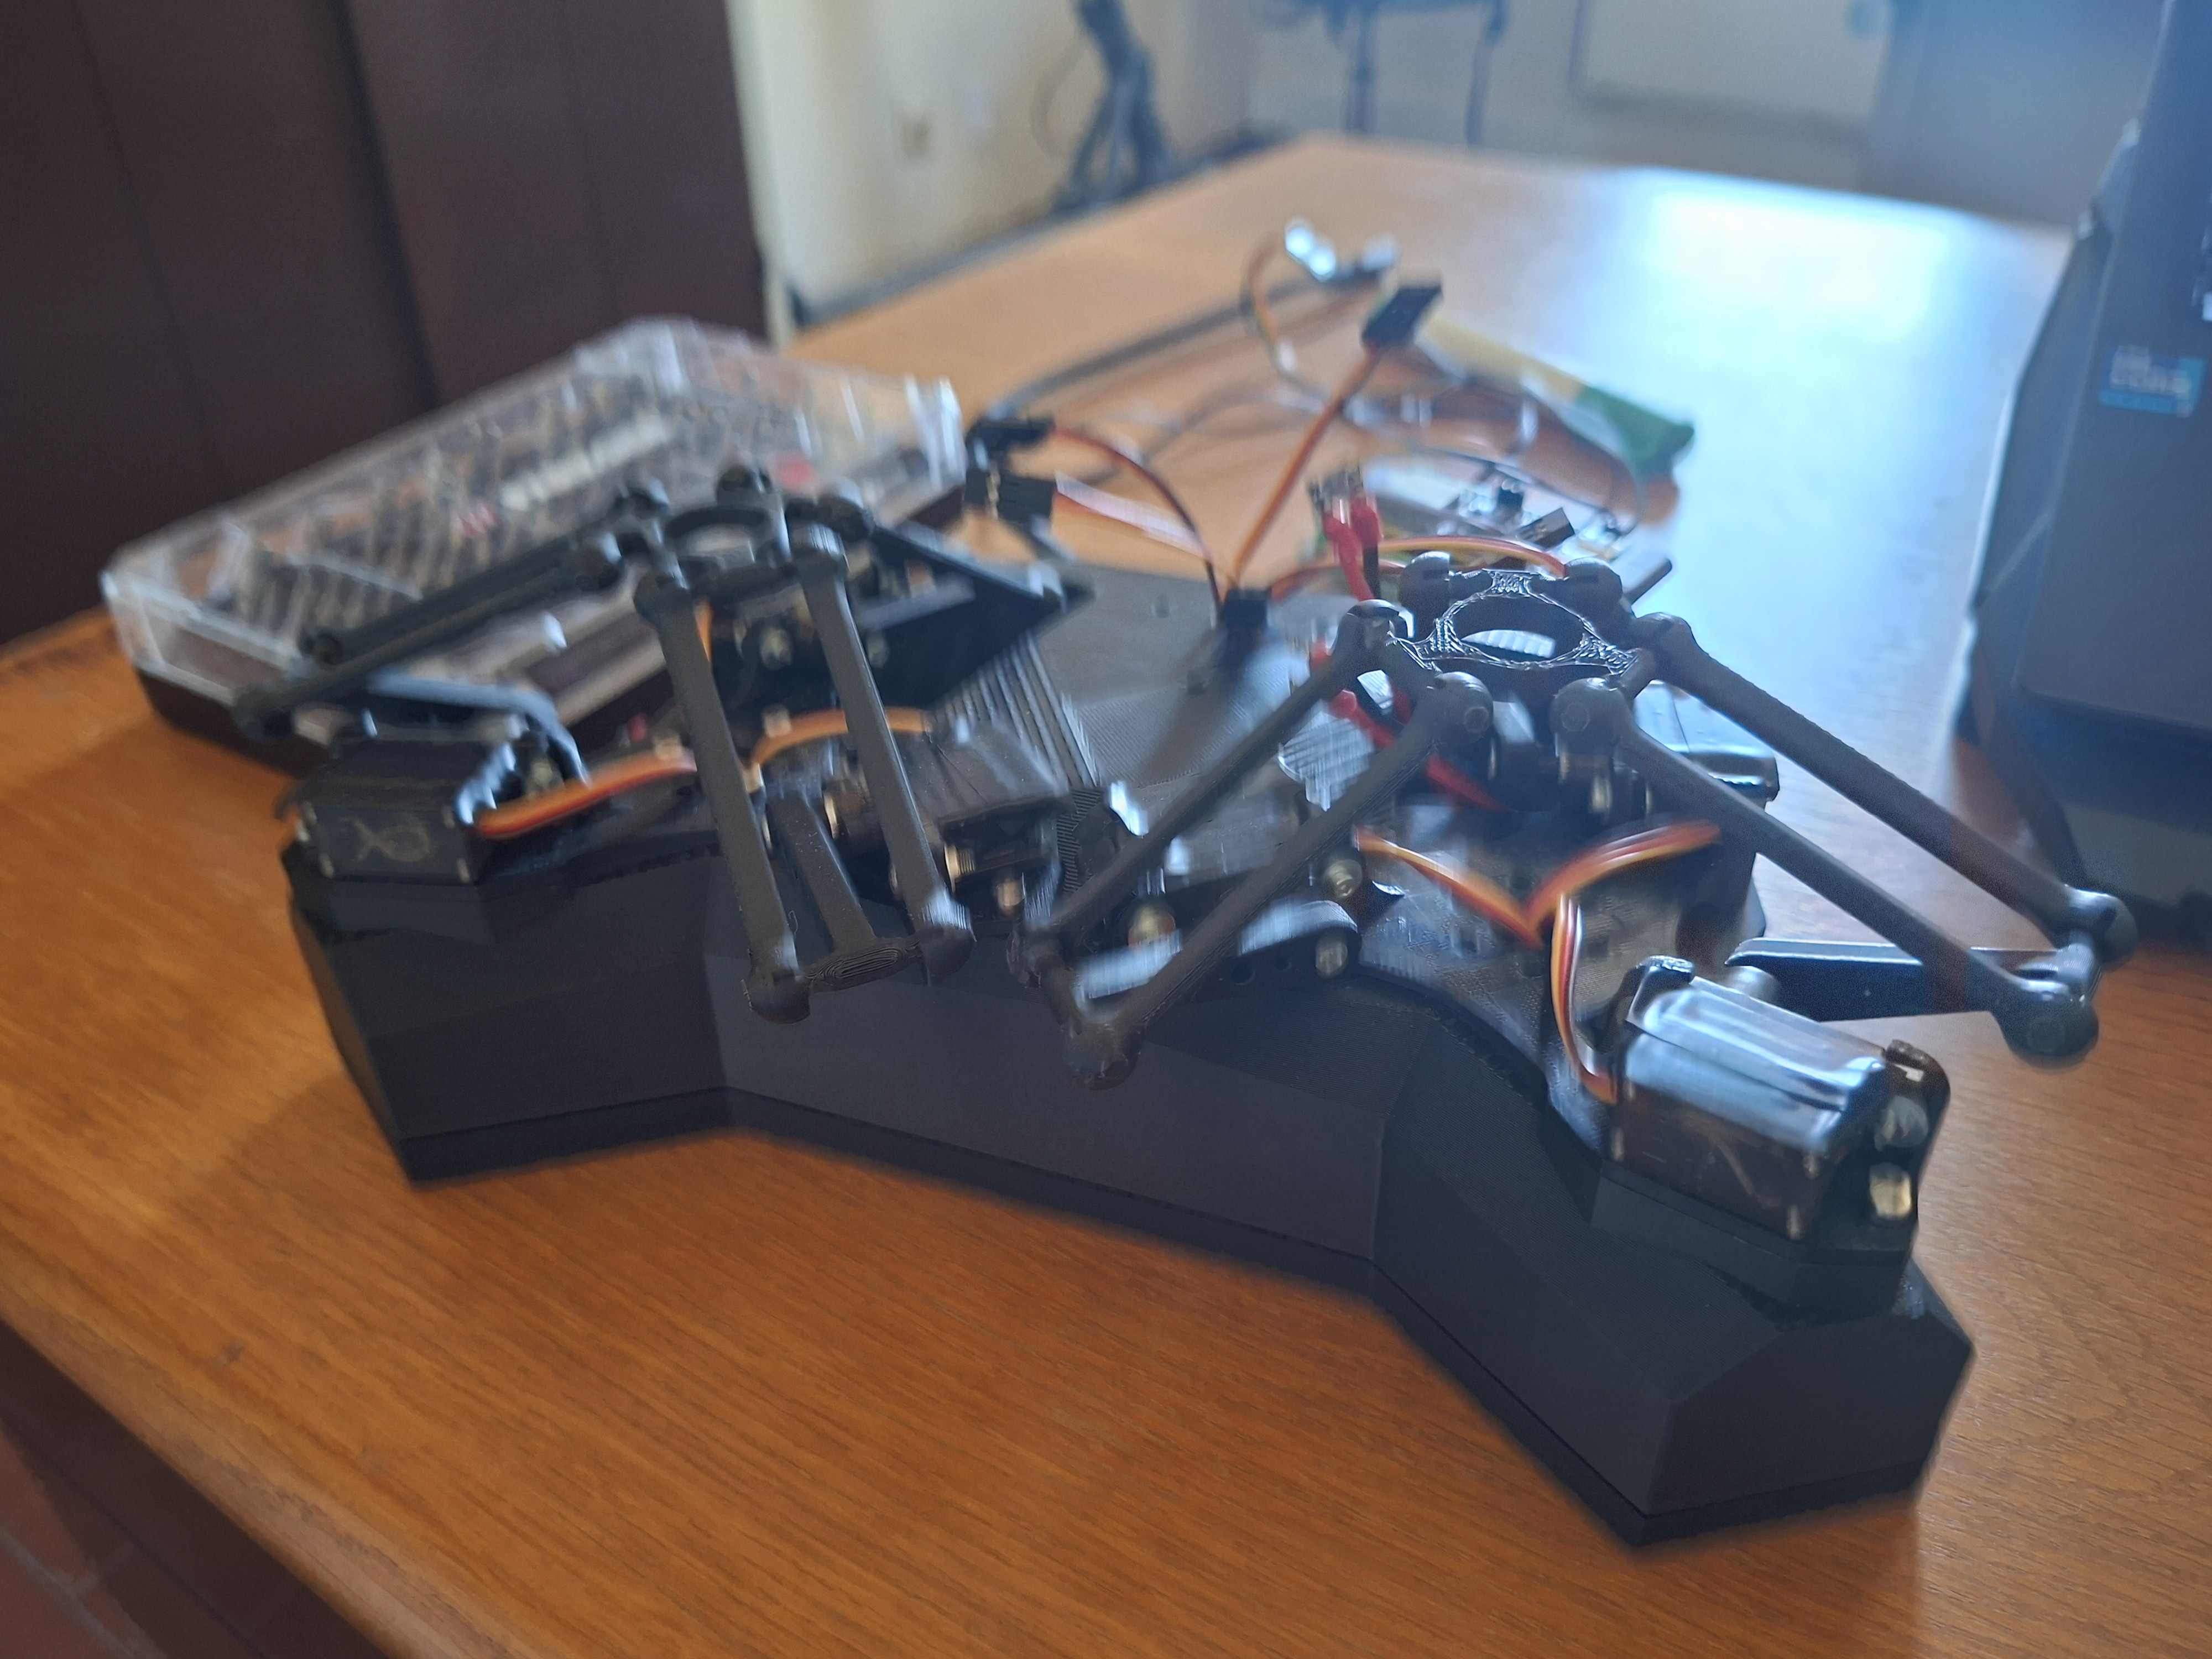
\includegraphics[width=0.72\textwidth]{fotos/delta_dois_manipuladores.jpg}
  \caption{Os dois manipuladores delta montados com os servos Waveshare instalados, prontos para calibração de firmware. Os cabos dos servos são visíveis mas ainda sem organização final de cablagem.}
  \label{fig:delta-dois-manipuladores}
\end{figure}

Para acomodar o Raspberry Pi 4B e a fonte de alimentação de forma compacta e robusta, foi projetada e impressa uma caixa em PLA branco. Esta estrutura, visível na \cref{fig:raspberry-pi-caixa}, agrupa o Raspberry Pi com a fonte de alimentação comutada numa única unidade que pode ser posicionada independentemente do modelo físico.

\begin{figure}[htbp]
  \centering
  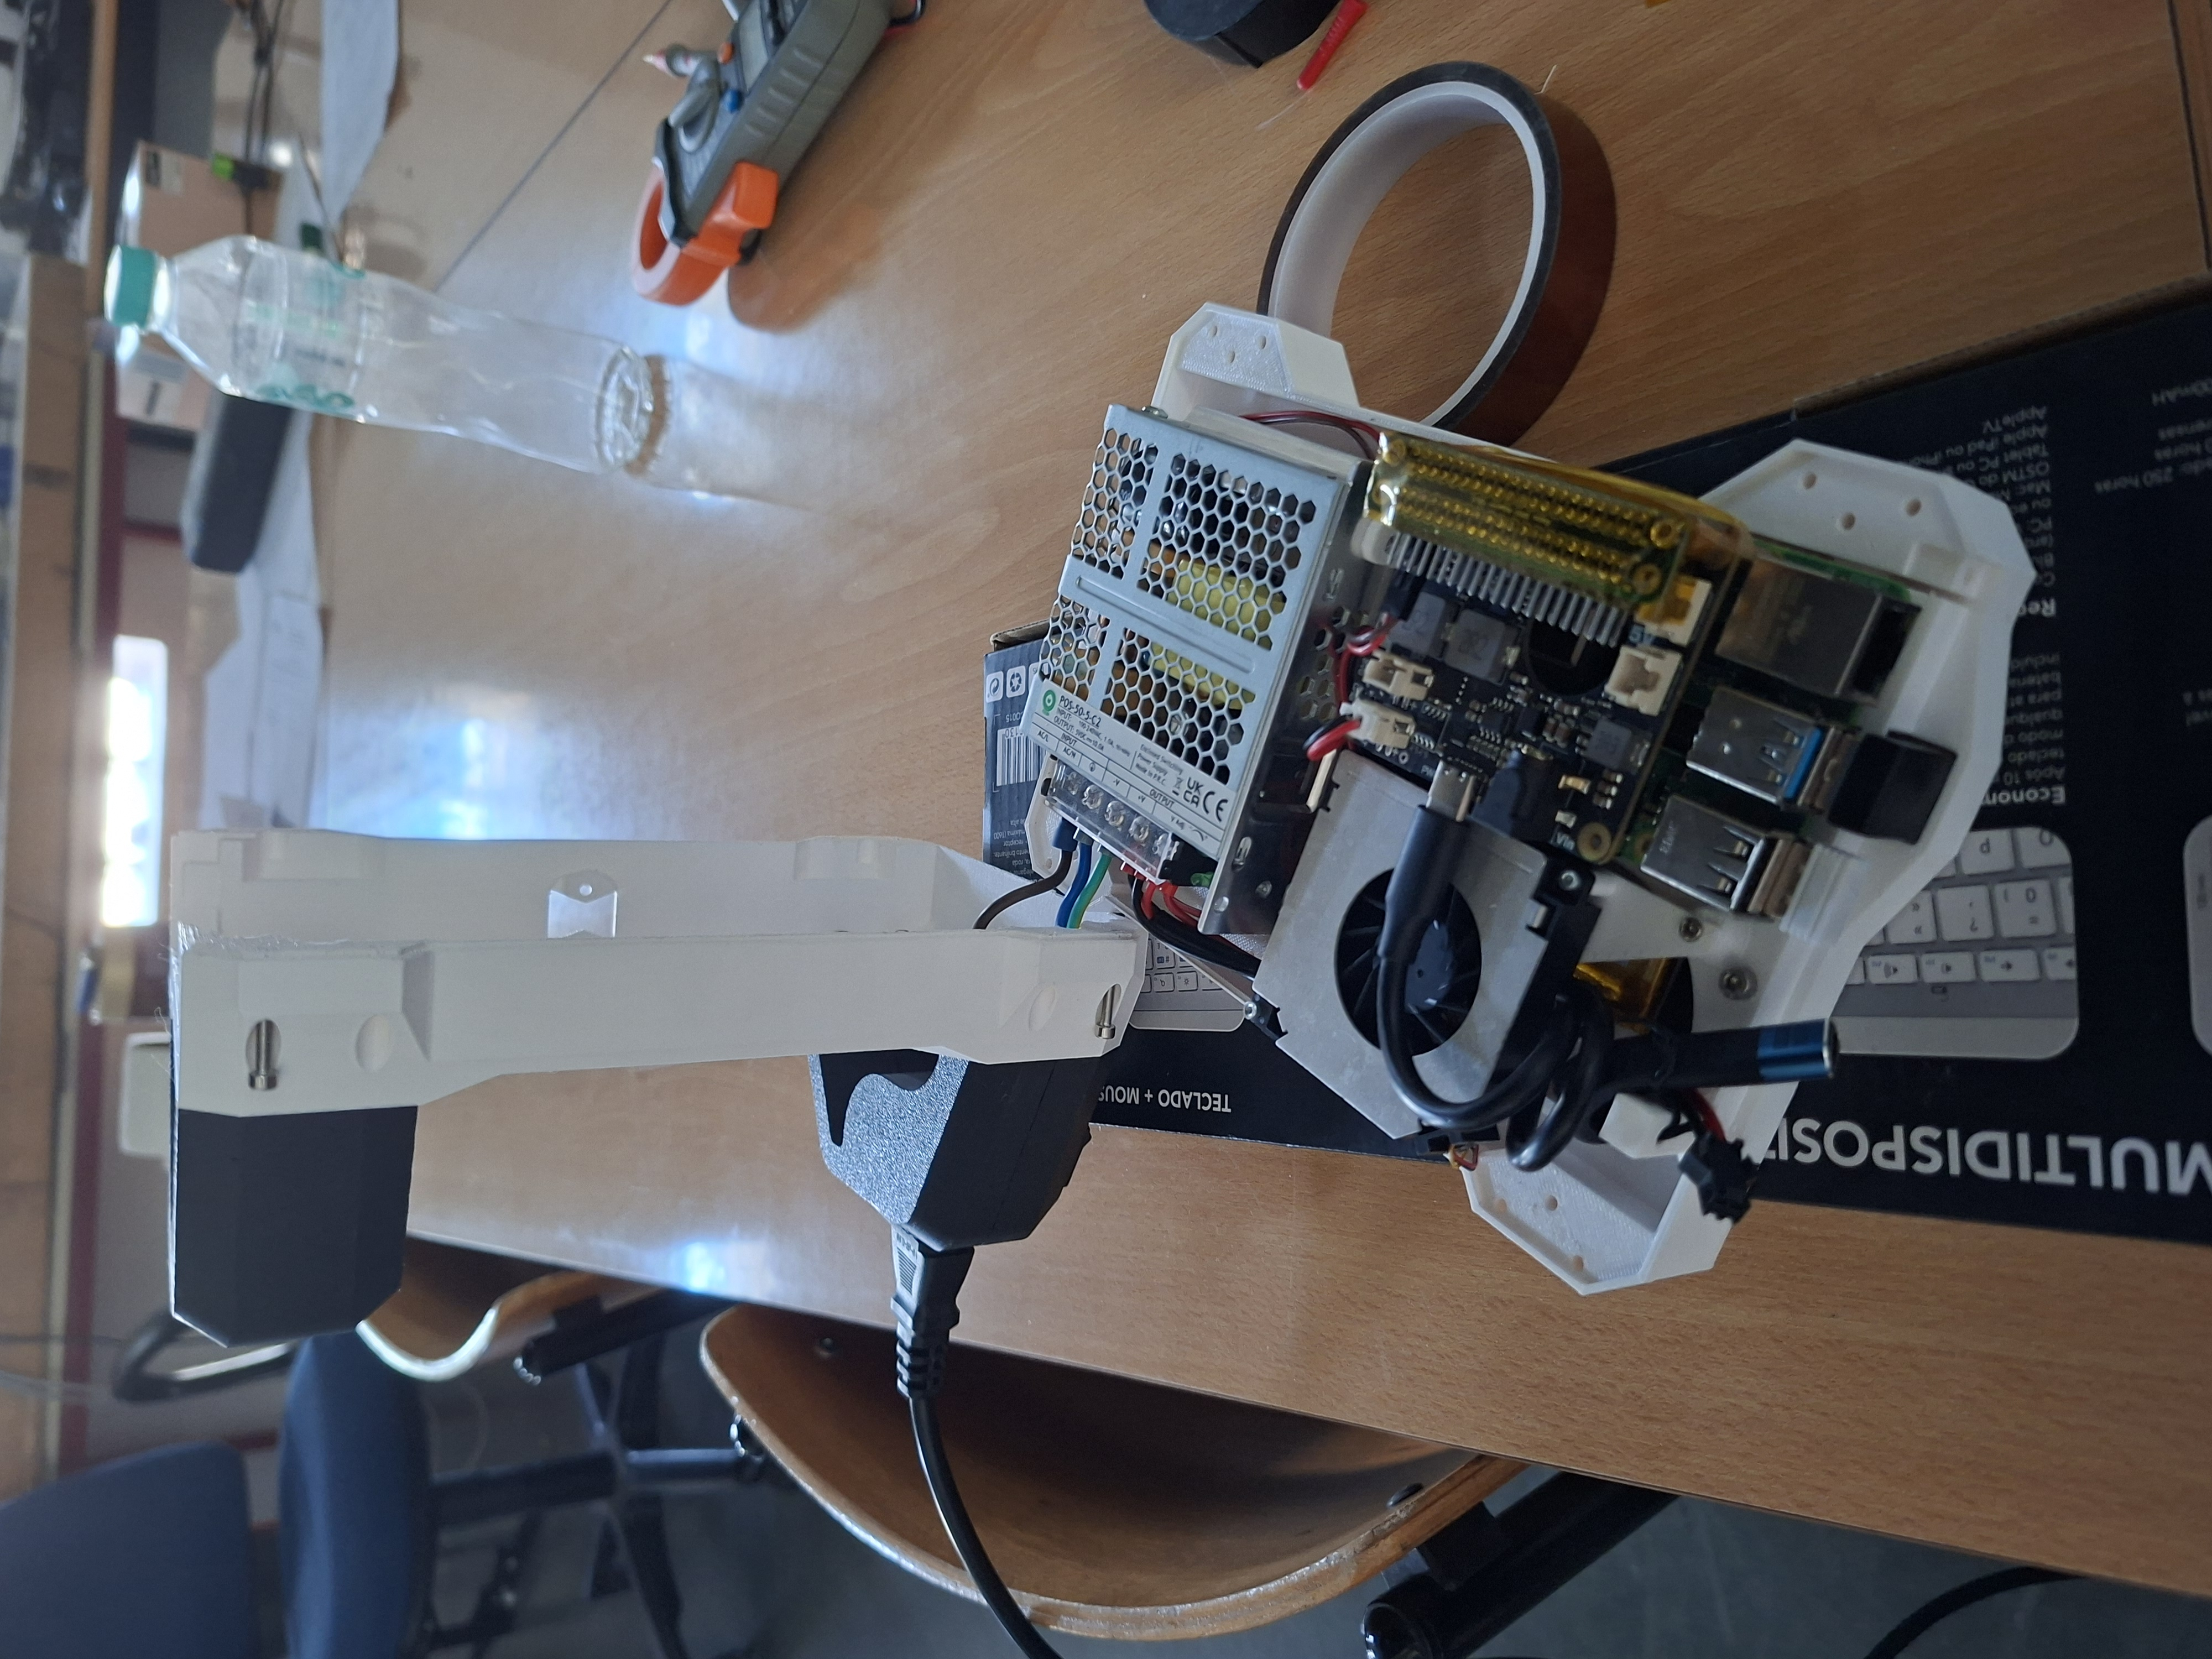
\includegraphics[width=0.72\textwidth]{fotos/raspberry_pi_caixa.jpg}
  \caption{Caixa impressa em PLA branco que aloja o Raspberry Pi 4B e a fonte de alimentação comutada.}
  \label{fig:raspberry-pi-caixa}
\end{figure}
\clearpage

\chapter{Desenvolvimentos do Software e Configurações}

O software foi desenvolvido em paralelo com o hardware, mas em camadas progressivas. Começou por testes elementares de comunicação série para confirmar que o ESP32 e o Raspberry Pi conseguiam trocar dados de forma fiável. A partir daí foram adicionados, um a um, os blocos de geração de trajetórias, de máquinas de estados, de cinemática inversa e de interface gráfica. Este capítulo descreve essa construção por partes, da arquitetura global até aos detalhes de calibração e sincronização, seguindo a ordem em que cada bloco foi desenvolvido e validado.

\section{Arquitetura geral do software e ambiente de desenvolvimento}
\label{sec:arquitetura-software-geral}
O software do projeto foi dividido em dois sistemas distintos que comunicam entre si através de um único canal de comunicação série bidirecional. O primeiro é o firmware do ESP32-S3, responsável pela execução e gestão física dos movimentos. 
O segundo é a HMI, alojada num Raspberry Pi 4B, responsável pela interação com o utilizador. 
A \cref{fig:esquema-global-software} ilustra esta relação de alto nível entre os dois sistemas.

\begin{figure}[htbp]
  \centering
  \begin{tikzpicture}[
    block/.style={draw, rounded corners=4pt, align=center, minimum width=4.5cm, minimum height=1.4cm, thick, font=\small}
  ]
    \node[block, fill=blue!12] (pi) at (0,0) {HMI\\Raspberry Pi 4B};
    \node[block, fill=green!10] (esp) at (13,0) {Firmware\\ESP32-S3};
    \draw[-Latex, ultra thick] ([yshift=0.5cm]pi.east) -- ([yshift=0.5cm]esp.west);
    \draw[-Latex, ultra thick] ([yshift=-0.5cm]esp.west) -- ([yshift=-0.5cm]pi.east);
    \node[font=\Large\bfseries, text=red, fill=white, inner sep=2pt] at ($(pi.east)!0.5!(esp.west)$) {comunicação série};
  \end{tikzpicture}
  \caption{Esquema global de comunicação entre o firmware do ESP32-S3 e a HMI no Raspberry Pi 4B.}
  \label{fig:esquema-global-software}
\end{figure}

O firmware do ESP32 foi inteiramente desenvolvido no ambiente PlatformIO, integrado no Visual Studio Code. Esta escolha surgiu numa altura de transição natural do projeto: durante muito tempo, a programação de microcontroladores tinha sido feita através do Arduino IDE, sempre em conjunto com placas Arduino, e a adoção do ESP32 neste projeto tornou-se a oportunidade ideal para migrar para um ambiente mais adequado. Ao contrário do Arduino IDE, que antigamente exigia a instalação de definições externas para reconhecer placas fora do ecossistema Arduino, o PlatformIO oferece suporte nativo à quase totalidade das placas atualmente disponíveis no mercado. A esta vantagem juntam-se ainda funcionalidades como sugestões inteligentes de código em tempo real, semelhantes a um sistema de auto-completar avançado, a integração direta com o Git através do próprio Visual Studio Code, a possibilidade de trabalhar simultaneamente com várias linguagens no mesmo ambiente e a verificação de erros em tempo real durante a escrita do código. Ainda que a curva de aprendizagem inicial seja mais exigente do que a do Arduino IDE, a prática rapidamente revela um ambiente de desenvolvimento consideravelmente mais poderoso e completo.

A HMI, por sua vez, foi inteiramente desenvolvida em Python 3, por ser uma linguagem com acesso a diversas bibliotecas dedicadas ao desenvolvimento de interfaces e aplicações, facilitando consideravelmente o processo de desenvolvimento.

O desenvolvimento da interface foi inicialmente repartido em pequenas funcionalidades independentes, começando apenas pelas mais importantes: a comunicação série do lado do Python, o cálculo de pontos das trajetórias e a estrutura principal da própria interface. Todo este desenvolvimento inicial foi executado e iterado no IDE Thonny, escolhido pela sua interface simples e pela curva de aprendizagem reduzida, adequada a esta fase inicial de testes. Mais tarde, todo o desenvolvimento em Python foi migrado para um ambiente dentro do próprio Visual Studio Code, o que permitiu reunir os códigos de ambos os sistemas e dispositivos, bem como todas as configurações e a documentação associada, num único repositório, facilitando o transporte, a execução e a partilha entre dispositivos, bem como o acompanhamento da evolução do projeto através do Git.

\section{Arquitetura do firmware ESP32-S3}
O firmware do ESP32-S3 foi concebido como um sistema independente de controlo em tempo real, responsável por receber e interpretar os comandos da HMI, gerir o estado interno dos movimentos, executá-los de forma coordenada e precisa e, por fim, converter as trajetórias pretendidas em sinais próprios para os atuadores dos manipuladores delta, os servo-motores MG90S. Por este motivo, a maior parte dos blocos mais importantes do código foram construídos recorrendo a máquinas de estados (FSM), uma abordagem que confere ao firmware uma natureza flexível e independente, sem comprometer a precisão nem a eficiência da execução.

Esta arquitetura não partiu do zero. O ponto de partida deste firmware foi um exemplo de referência para manipuladores delta, disponível publicamente, sendo adaptado à geometria e aos servos usados neste projeto. Depois de confirmado o funcionamento básico da cinemática e do acionamento individual dos servos, esse código de referência foi sendo progressivamente modificado e organizado para complementar as necessidades do porjeto á medida que era introduzidos os outros blocos de funções de forma separados do resto do funcionamento do código, o que permitiu reescrever cada bloco, estruturas de dados, geração de movimento e máquinas de estados de forma independente.

O código está assim organizado em dois tipos de blocos: blocos de máquinas de estados e blocos de funções. Entre as FSM contam-se a \texttt{FSM\_Serial\_Reader}, a \texttt{FSM\_Serial\_Command}, a \texttt{FSM\_Tosse\_trigger}, a \texttt{FSM\_Monitor\_trigger}, a \texttt{FSM\_Preparação\_Tosse} e, sobretudo, a \texttt{FSM\_Motion\_update}, responsável pela execução dos movimentos. Entre os blocos de funções destacam-se a \texttt{Intermed\_position()}, a \texttt{Fusao\_plus\_IK\_D1()} e a \texttt{Fusao\_plus\_IK\_D2()}, além das estruturas de dados que suportam todo o código, como \texttt{Coordinate}, \texttt{MotionStorage} e \texttt{MotionInstance}.

Muitos destes blocos foram construídos de forma flexível face ao tipo de variáveis com que trabalham, permitindo reutilizar uma única função para vários tipos de movimento em situações distintas, sem replicar a mesma lógica várias vezes. É o caso da \texttt{FSM\_Motion\_update} e da \texttt{Intermed\_position}, chamadas de forma independente para a respiração, o batimento cardíaco e a tosse, alterando apenas os parâmetros e as trajetórias associadas a cada caso.

\begin{figure}[p]
  \centering
  \resizebox{\textwidth}{!}{%
  \begin{tikzpicture}[
    block/.style={draw, rounded corners=3pt, align=center, minimum width=3.0cm, minimum height=1.1cm, thick, font=\scriptsize},
    small/.style={draw, rounded corners=3pt, align=center, minimum width=1.25cm, minimum height=0.65cm, thick, font=\scriptsize},
    arrow/.style={-Latex, thick},
    cfg/.style={-Latex, thick, green!60!black},
    event/.style={-Latex, thick, red!70!black},
    positionflow/.style={-Latex, thick, orange!85!black},
    lab/.style={font=\tiny, fill=white, inner sep=1pt}
  ]
    \node[block, fill=blue!12]  (pi)     at (-6.5,24.0) {Raspberry\\Pi 4B};
    \node[block, fill=cyan!10]  (reader) at (-6.5,20.0) {FSM\_Serial\\\_reader};
    \node[block, fill=cyan!10]  (interp) at (-1.5,20.0) {FSM\_Serial\\\_Command};
    \node[block, fill=gray!12]  (eeprom) at (-1.5,24.0) {Gravação\\memória EEPROM};

    \node[block, fill=red!8]   (ttrig) at (4.0,24.0) {FSM\_Tosse\\\_trigger};
    \node[block, fill=red!6]   (tmon)  at (5.7,21.9) {FSM\_Monitor\\\_trigger};
    \node[block, fill=red!10]  (tprep) at (4.0,19.2) {FSM\_Preparação\\\_Tosse};

    \node[block, fill=green!10] (mresp)  at (-6.5,15.5) {FSM\_Motion\_update\\(Respiração)};
    \node[block, fill=green!10] (mbat)   at (-1.5,15.5) {FSM\_Motion\_update\\(Batimento)};
    \node[block, fill=green!10] (mtosse) at (4.0,15.5)  {FSM\_Motion\_update\\(Tosse)};

    \node[block, fill=orange!10] (ipresp)  at (-6.5,11.5) {Intermed\\\_position};
    \node[block, fill=orange!10] (ipbat)   at (-1.5,11.5) {Intermed\\\_position};
    \node[block, fill=orange!10] (iptosse) at (4.0,11.5)  {Intermed\\\_position};

    \node[block, fill=orange!16] (fus1) at (-4.0,7.5) {Fusao\_plus\\\_IK\_D1};
    \node[block, fill=orange!16] (fus2) at (1.5,7.5)  {Fusao\_plus\\\_IK\_D2};

    \node[small, fill=yellow!20] (s11) at (-5.5,4.0) {\(\theta_1\)};
    \node[small, fill=yellow!20] (s12) at (-4.0,4.0) {\(\theta_2\)};
    \node[small, fill=yellow!20] (s13) at (-2.5,4.0) {\(\theta_3\)};
    \node[small, fill=yellow!20] (s21) at (0.0,4.0)  {\(\theta_1\)};
    \node[small, fill=yellow!20] (s22) at (1.5,4.0)  {\(\theta_2\)};
    \node[small, fill=yellow!20] (s23) at (3.0,4.0)  {\(\theta_3\)};

    \coordinate (busX) at (-1.0,9.5);

    \draw[arrow] (pi) -- (reader);
    \draw[arrow] (reader) -- node[lab, above]{CH\_Command} (interp);
    \draw[cfg] (interp.north) -- node[lab, left]{config} (eeprom.south);
    \draw[cfg] (eeprom.east) -- ++(0.9,0) |- node[lab, pos=0.1, above]{leitura} (interp.east);
    \draw[arrow] (interp.south west) ++(-0.15,0) -- ++(0,-1.4) -| node[lab, pos=0.2, above]{ativa} (mresp.north);
    \draw[arrow] (interp.south) -- node[lab, right]{ativa} (mbat.north);
    \draw[arrow] (interp.south east) ++(0.15,0) -- ++(0,-1.4) -| node[lab, pos=0.8, above]{ativa} (mtosse.north);
    \draw[event] (ttrig.east) to[out=-20,in=90] node[lab, pos=0.3, right]{sinal\_tossir} (tmon.north);
    \draw[event] (tmon.south) to[out=-100,in=20] node[lab, pos=0.7, below right]{validado} (tprep.east);
    \draw[event] (tprep.south west) ++(-0.2,0) -- ++(0,-1.6) -| node[lab, pos=0.15, above]{modula período/amplitude} (mresp.north east);
    \draw[event] (tprep) -- node[lab, right]{ativa vibração} (mtosse);
    \draw[arrow] (mresp) -- (ipresp);
    \draw[arrow] (mbat) -- (ipbat);
    \draw[arrow] (mtosse) -- (iptosse);
    \draw[positionflow] (ipresp.south) -- ++(0,-1.3) -| (busX);
    \draw[positionflow] (ipbat.south) -- ++(0,-1.3) -| (busX);
    \draw[positionflow] (iptosse.south) -- ++(0,-1.3) -| (busX);
    \draw[positionflow] (busX) -- ++(0,-1.3) -| node[lab, pos=0.2, above]{Lerp\_Respi/Batim/Tosse\_OUT} (fus1.north);
    \draw[positionflow] (busX) -- ++(0,-1.3) -| (fus2.north);
    \draw[arrow] (fus1) -- (s11);
    \draw[arrow] (fus1) -- (s12);
    \draw[arrow] (fus1) -- (s13);
    \draw[arrow] (fus2) -- (s21);
    \draw[arrow] (fus2) -- (s22);
    \draw[arrow] (fus2) -- (s23);
  \end{tikzpicture}}
  \caption{Estrutura global das máquinas de estados e blocos de controlo do firmware.}
  \label{fig:arquitetura-software}
\end{figure}
\clearpage

O percurso dos dados começa na \texttt{FSM\_Serial\_Reader}, que funciona como camada de receção global, recolhendo os caracteres vindos da HMI sem perturbar a execução dos movimentos. Depois de recebidos, os comandos são redirecionados, um caracter de cada vez ou numa única sequência de texto, para a \texttt{FSM\_Serial\_Command}, onde são distinguidos comandos simples, como o arranque, a paragem, a seleção de modo, a gravação e leitura de dados na memória EEPROM ou até a verificação dos dados nas estruturas internas, dos comandos-chave parametrizados, usados apenas para alterar e atualizar informações de configuração e definições. É através destes últimos que são atualizadas as flags de funcionamento e as estruturas de movimento, refletindo de imediato qualquer alteração na configuração ativa do sistema.

Em paralelo, a \texttt{FSM\_Motion\_update} de cada fenómeno fisiológico ativo (respiração, batimento cardíaco e vibração da tosse) percorre a respetiva trajetória discreta, usando apenas índices, direção, pausas e tempos internos. A \texttt{FSM\_Tosse\_trigger}, a \texttt{FSM\_Monitor\_trigger} e a \texttt{FSM\_Preparação\_Tosse} funcionam em conjunto como uma camada intermédia entre o comando recebido e a execução física da tosse, ajustando temporariamente a respiração e ativando a componente de vibração sempre que o evento é gerado.

Nesta fase, as posições de cada movimento ainda são apenas índices, sem qualquer significado direto para os manipuladores. Por isso os dados dos indices são redirecionados para a função \texttt{Intermed\_position}, onde são convertidos em valores de real significado (coordenadas cartesianas). Em sequancia a esta connversão são assiociados os valores do indice atual e o indice futuro e calculado uma coordenada intermédia (interpolação) entre o ponto atual e o próximo, em função do tempo decorrido e do tempo até ao ponto seguinte, resultando numa saída de posições limpa, suave e precisa ao longo de toda a simulação.

No final do sistema, os blocos de fusão de coordenadas e de cinemática inversa, \texttt{Fusao\_plus\_IK\_D1} e \texttt{Fusao\_plus\_IK\_D2}, reúnem toda a informação proveniente dos movimentos ativos e convertem a posição resultante (ainda em coordenadas cartesiansas), nos ângulos a alcançar em tempo real por cada um dos atuadores dos dois manipuladores delta.

\begin{figure}[H]
  \centering
  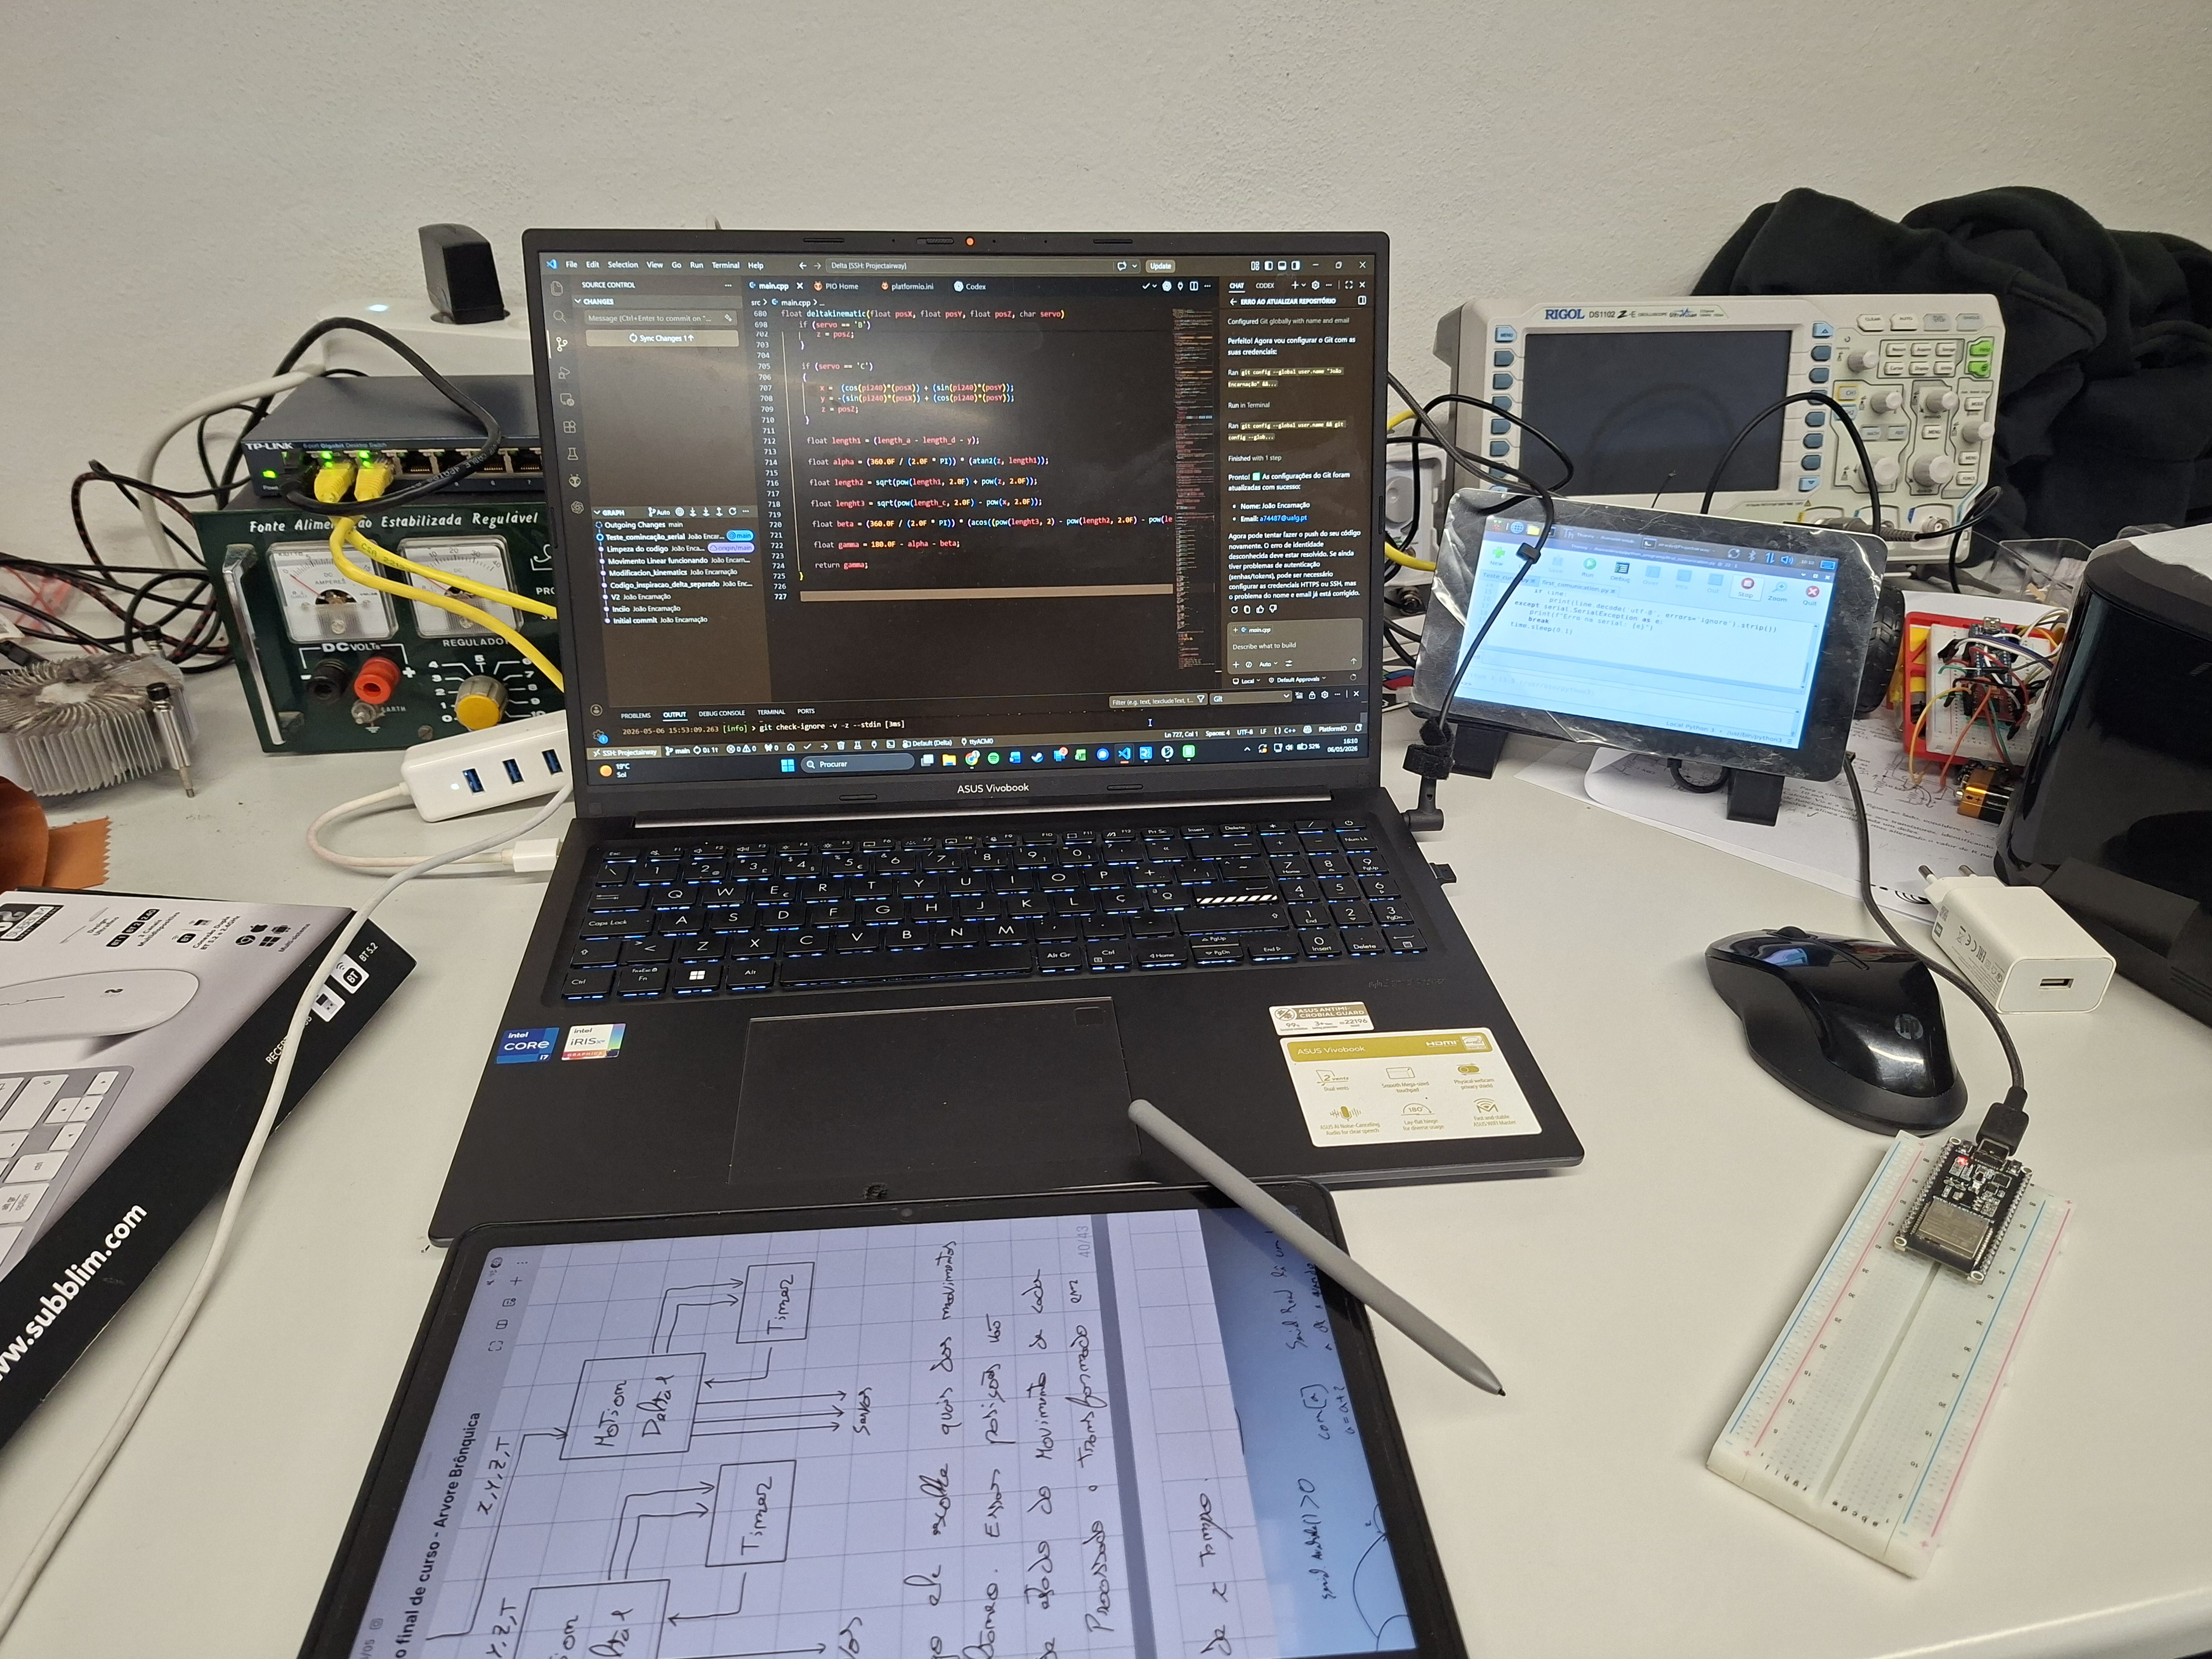
\includegraphics[width=0.78\textwidth]{fotos/ambiente_desenvolvimento.jpg}
  \caption{Desenvolvimento da arquitetura principal do ESP32.}
  \label{fig:ambiente-desenvolvimento}
\end{figure}

\clearpage
\section{Movimentos representados no protótipo}
O estado da arte identificou vários movimentos observáveis durante a broncoscopia. No entanto, para o projeto, foram selecionados apenas os movimentos com melhor relação entre relevância clínica, viabilidade mecânica e simplicidade de controlo: respiração, batimento cardíaco e tosse. Os valores de frequência e amplitude usados nas secções seguintes, resumidos na \cref{tab:movimentos-hardware}, foram retirados diretamente do documento de trabalho fornecido pela equipa de Pneumologia do CHUA \parencite{Santos2026}.

\begin{table}[htbp]
  \centering
  \caption{Movimentos considerados para o projeto.}
  \label{tab:movimentos-hardware}
  \begin{tabular}{@{}p{3.0cm}p{3.0cm}p{3.0cm}p{4.4cm}@{}}
    \toprule
    Movimento & Frequência & Amplitude prevista & Observações \\
    \midrule
    Respiração & 12--20 ciclos/min & 5--\SI{15}{\milli\metre} & Predominantemente craniocaudal, com uma componente lateral associada \\
    Batimento cardíaco & 60--120 bpm & 1--\SI{3}{\milli\metre} & Compressão direcional localizada, com contração breve e pausa variável \\
    Tosse & Evento curto & 5--\SI{25}{\milli\metre} & Abrupto e irregular, altera temporariamente a respiração \\
    \bottomrule
  \end{tabular}
\end{table}

A respiração foi descrita com base num deslocamento predominantemente craniocaudal (vertical), como um movimento cíclico, de frequência aproximada de 12 a 20 ciclos por minuto e amplitude extensa, de cerca de 5 a \SI{15}{\milli\metre}. A este deslocamento principal associa-se ainda uma componente lateral de menor magnitude, confirmada em modelos computacionais do movimento brônquico ao longo do ciclo respiratório, nos quais o deslocamento lateral surge sistematicamente depois da predominância craniocaudal \parencite{Kim2023}. Do ponto de vista da modelação, esta componente lateral pode ser entendida como resultante do facto de a árvore brônquica não acompanhar em linha reta o movimento vertical imposto pelo diafragma, e sim deslizar lateralmente de forma percetível à medida que a base pulmonar desce e sobe, o que resulta numa trajetória com uma curvatura suave em vez de um simples deslocamento vertical linear.

Já o batimento cardíaco foi associado a um deslocamento predominante no brônquio principal esquerdo, devido à proximidade anatómica do coração, prevendo-se um movimento de baixa amplitude, cerca de 1 a \SI{3}{\milli\metre}, com frequência aproximada de 60 a 120 batimentos por minuto. Esta proximidade leva a que o coração e os vasos sanguíneos junto dele entrem em contacto direto com o brônquio, comprimindo-o periodicamente a cada batimento, um efeito também documentado em observações por broncoscopia \parencite{Arcieri2016} e confirmado junto da equipa de Pneumologia do CHUA. A compressão resultante afeta tipicamente o brônquio como um todo e não apenas um ponto localizado, ocorrendo preferencialmente na direção lateral, com uma contribuição secundária no sentido ântero-posterior, em vez de se distribuir uniformemente em torno da sua circunferência \parencite{Santos2026}. Por essa razão, o percurso do movimento cardíaco não é um simples movimento retilíneo, traçando antes um pequeno percurso fechado a cada ciclo. No protótipo, este movimento foi por isso representado como uma oscilação fechada, alongada preferencialmente na direção lateral, sobreposta ao movimento respiratório.

O ciclo cardíaco em si também não é temporalmente simétrico, sendo composto por duas fases principais. A fase sistólica (o momento de contração do coração) tem uma duração absoluta, relativamente curta, mantendo-se na ordem das poucas centenas de milissegundos. Pelo contrário, é a fase diastólica (o intervalo de repouso entre contrações sucessivas), que absorve quase toda a variação do período à medida que a frequência cardíaca aumenta, encolhendo de forma muito mais acentuada do que a sístole \parencite{Chung2004}. Esta relação entre uma contração breve e praticamente constante e uma pausa mais longa e variável consoante a frequência cardíaca foi também confirmada junto da equipa de Pneumologia do CHUA. Contudo, esta variação periódica, tanto na respiração como no batimento cardíaco, não foi replicada no projeto, tendo-se optado por uma oscilação de velocidade constante ao longo de todo o período de treino, de modo a simplificar o cálculo e a calibração do movimento sem comprometer o seu contributo visual (sendo ainda possível alterar os valores de período, mas apenas fora da execução de treino).

A tosse foi caracterizada como um evento abrupto, irregular e de maior amplitude relativa e, em vez de ser apenas uma trajetória independente, deve alterar temporariamente o comportamento respiratório, aumentando a amplitude e introduzindo uma perturbação rápida.

\section{Geração de trajetórias (Python/Raspberry Pi)}
\label{sec:geracao-trajetorias}
Com os requisitos clínicos de cada movimento já definidos na secção anterior, o passo seguinte consistiu em traduzir essa descrição qualitativa em trajetórias discretas, calculáveis e executáveis pelo modelo.

Essa tradução foi implementada inteiramente em ambiente de Python com auxílio da biblioteca matplotlib, sendo responsável por transformar os parâmetros configuráveis de cada movimento, primeiramente em curvas, de seguida em pontos e finalmente em gráficos que futuramente seriam reaproveitados e apresentados diretamente na HMI. Este cálculo foi inicialmente desenvolvido fora da componente de interface, para permitir validar, ainda numa fase inicial do desenvolvimento de hardware e software, a geração de curvas e de pontos em coordenadas cartesianas admissíveis para posterior inserção no firmware do ESP32. Uma decisão de arquitetura particularmente relevante nesta fase foi a escolha de descrever cada movimento recorrendo apenas a um plano 2D específico do espaço 3D do manipulador (por exemplo, XY, XZ ou YZ), em vez de calcular antecipadamente, em Python, a fusão completa de todos os movimentos numa única trajetória tridimensional já pronta para o manipulador. Esta segunda abordagem foi de facto a primeira ideia considerada e manteve-se como hipótese de trabalho durante bastante tempo, consistindo em gerar previamente uma trajetória global fundida, resultando numa única matriz de posições a enviar ao manipulador.

Esta abordagem revelou-se, no entanto, pouco flexível para desenvolvimentos futuros, uma vez que exigiria que o período do batimento cardíaco fosse sempre um múltiplo inteiro do período da respiração, de modo a que a trajetória fundida se repetisse de forma consistente ao longo do tempo. Como os dois movimentos não têm uma relação de período exata entre si, cada secção da trajetória teria um tempo diferente, tornando impossível prever antecipadamente, ao longo do array de pontos, todos os instantes em que o batimento poderia ocorrer relativamente à respiração. No caso da tosse, cuja ocorrência é ainda menos previsível, esta abordagem seria mesmo impossível.

A possibilidade de descrever cada movimento recorrendo apenas a um plano 2D específico, dentro do espaço 3D mais amplo do manipulador, resolveu este problema. Esta escolha permitiu transferir a etapa de fusão dos movimentos para o próprio ESP32, executando-a quase em tempo real e possibilitando que modificações e eventos, como a tosse, ocorressem diretamente sobre essa fusão, sem necessidade de calcular antecipadamente planos ou simulações complexas para um único movimento universal do manipulador.

\subsection{Desenvolvimento e iterações}
Estabelecida esta decisão de arquitetura, passou-se para a execução, validação e iteração sucessiva do cálculo de cada curva, dando-se início com a implementação da geração de curvas e cálculo de pontos, sendo o batimento cardíaco o primeiro movimento de todos a ser descrito e testado em formato de curva no script. Foi utilizada a fórmula de uma elipse para descrever o deslocamento cardíaco, definida por dois parâmetros geométricos principais, o comprimento e a largura, que permitiam controlar diretamente o formato da curva através dos semieixos \(a\) e \(b\):
\[
x_0(u) = a\cos(u), \qquad y_0(u) = b\sin(u).
\]
Esta elipse-base necessitou ainda de duas características adicionais: a capacidade de se posicionar em qualquer ponto do gráfico (para permitir recentrar a curva relativamente à origem) e a capacidade de rodar em torno desse mesmo ponto central.

A rotação foi implementada com base na matriz de rotação convencional,
\[
R(\alpha) =
\begin{bmatrix}
\cos(\alpha) & -\sin(\alpha) \\
\sin(\alpha) & \cos(\alpha)
\end{bmatrix},
\]
aplicada ao ponto \((x_0(u),y_0(u))\) da elipse-base, resultando em
\[
\begin{bmatrix} x_r(u) \\ y_r(u) \end{bmatrix}
= R(\alpha)\begin{bmatrix} x_0(u) \\ y_0(u) \end{bmatrix}
= \begin{bmatrix} a\cos(u)\cos(\alpha) - b\sin(u)\sin(\alpha) \\ a\cos(u)\sin(\alpha) + b\sin(u)\cos(\alpha) \end{bmatrix}.
\]

Por fim, a posição da elipse no gráfico é determinada pelas coordenadas \((x_c,y_c)\), correspondentes ao centro da elipse. Este deslocamento é livre e completamente independente da rotação \(R(\alpha)\): o ângulo \(\alpha\) orienta apenas a forma da elipse em torno do seu próprio centro, podendo esse centro ser colocado em qualquer ponto do gráfico. Só na função completa, apresentada adiante, estas coordenadas são somadas ao ponto já rodado da elipse, posicionando a elipse rodada no local pretendido do gráfico.

Na segunda iteração foi acrescentada a curva parabólica usada pela respiração e pela tosse que, por se apresentar no plano \(ZX\), exigiu duas correções: garantir que a parábola abria sempre no sentido de \(Z^+\) (de acordo com o sentido físico do movimento representado) e ajustar a escala dos eixos gráficos para que a proporção da curva fosse mantida corretamente, através do comando \texttt{set\_aspect('equal', adjustable='box')} em vez de \texttt{axis('equal')}, este último incompatível com os limites de eixo definidos manualmente. A curva base, comum aos dois movimentos, é dada por:
\[
X_0(u) = u, \qquad Z_0(u) = \frac{H}{L^2}u^2, \qquad 0 \leq u \leq L,
\]
em que \(H\) é a altura máxima e \(L\) é a largura máxima. Na terceira versão foi introduzido um sistema de controlo do sentido do percurso na curva elíptica do batimento cardíaco (horário ou anti-horário). Nesta fase, sempre que os valores de \(a\) e \(b\) eram alterados, o reposicionamento da elipse, de modo a manter o vértice de referência junto à origem do gráfico, tinha ainda de ser feito manualmente, ajustando \(x_c\) e \(y_c\).

\subsection{Módulo final}
Com todas as bases implementadas, foi construído em torno delas o módulo \texttt{calculo\_movimentos.py}, que permite introduzir parâmetros geométricos, o número de pontos e outras calibrações. Através de fórmulas específicas para cada movimento, este módulo devolve sequências de coordenadas no espaço tridimensional, numa ordem e orientação específicas, já preparadas para serem utilizadas e fundidas no firmware do ESP32.

De forma geral, cada movimento é definido por uma curva contínua \(\mathbf{p}(u)\) e por um conjunto discreto de \(N\) pontos:
\begin{equation}
  \mathbf{p}_i =
  \begin{bmatrix}
    X_i\\Y_i\\Z_i
  \end{bmatrix}
  =
  \mathbf{p}(u_i),
  \qquad i=0,1,\ldots,N-1.
\end{equation}

No módulo \texttt{calculo\_movimentos.py}, a posição da elipse do batimento cardíaco passou a ser descrita por um deslocamento orbital, em vez das coordenadas independentes \((x_c,y_c)\) das versões anteriores, com o objetivo de facilitar o cálculo e a parametrização da curva. Nesta representação, o centro da elipse é definido por uma distância \(R\) à origem do gráfico e pelo mesmo ângulo \(\alpha\) usado anteriormente, sendo a orientação da própria elipse dada por \(\alpha+\delta\), em que \(\delta\) é um pequeno ajuste fino da rotação interna da elipse (por padrão, \(\delta=0^\circ\)). A curva final é dada por:
\begin{align}
  X(u) &= R\cos(\alpha) + a\cos(u)\cos(\alpha+\delta) - b\sin(u)\sin(\alpha+\delta),\\
  Y(u) &= R\sin(\alpha) + a\cos(u)\sin(\alpha+\delta) + b\sin(u)\cos(\alpha+\delta),\\
  Z(u) &= 0,
\end{align}
\[
\{0 \leq u < 2\pi\}
\]
podendo o sentido de percurso ser horário ou anti-horário. Para manter o vértice de referência da elipse sempre ancorado junto à origem do gráfico, independentemente do ângulo \(\alpha\) escolhido, o valor de \(R\) é calculado automaticamente a partir de \(a\), \(b\) e \(\delta\):
\[
R = \frac{ab}{\sqrt{b^2\cos^2(\delta) + a^2\sin^2(\delta)}}.
\]
No conjunto de parâmetros usado nos testes da interface, foram considerados os diâmetros \(a=3\,mm\) e \(b=1,5\,mm\), \(\delta=0^\circ\), \(\alpha=20^\circ\), \(N=16\) pontos, sentido horário e um período \(T=0,75\,s\), correspondente a uma frequência cardíaca de 80 batimentos por minuto dentro do intervalo considerado. Para estes parâmetros, o valor de \(R\) calculado automaticamente foi \(R=1,50\,mm\).

\begin{figure}[H]
  \centering
  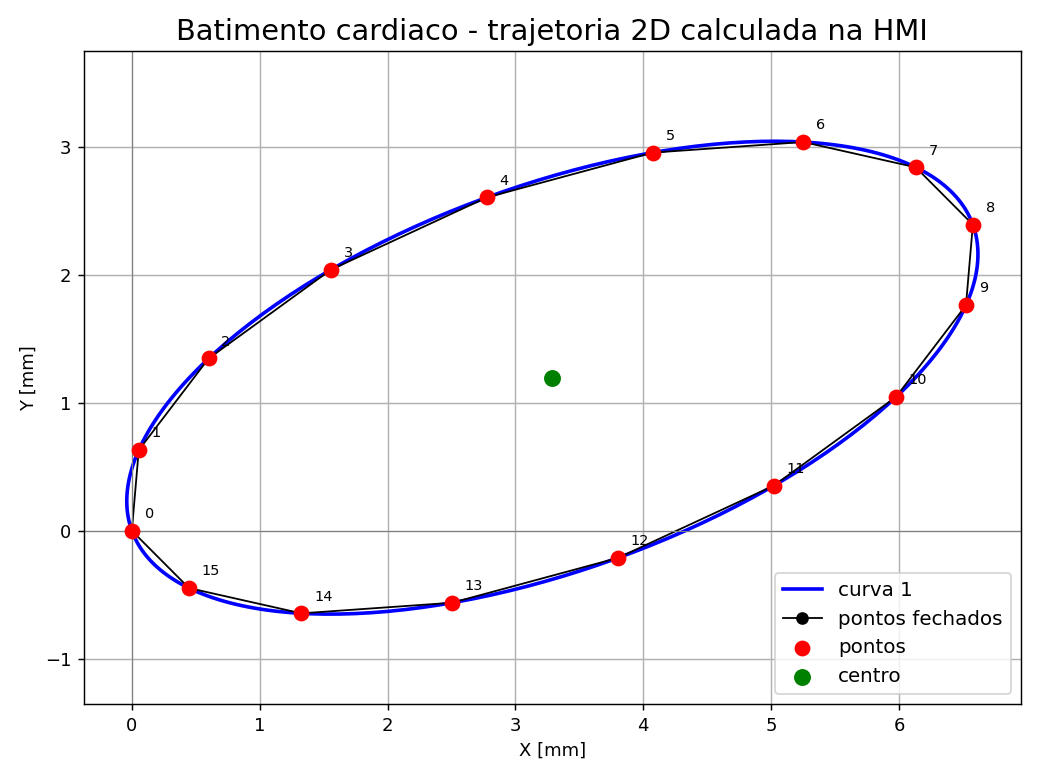
\includegraphics[width=0.62\textwidth]{movimentos/movimento_batimento_2d.png}
  \caption{Trajetória calculada para o movimento de batimento cardíaco, representação 2D dos pontos de passagem.}
  \label{fig:movimento-batimento-2d}
\end{figure}

\begin{figure}[H]
  \centering
  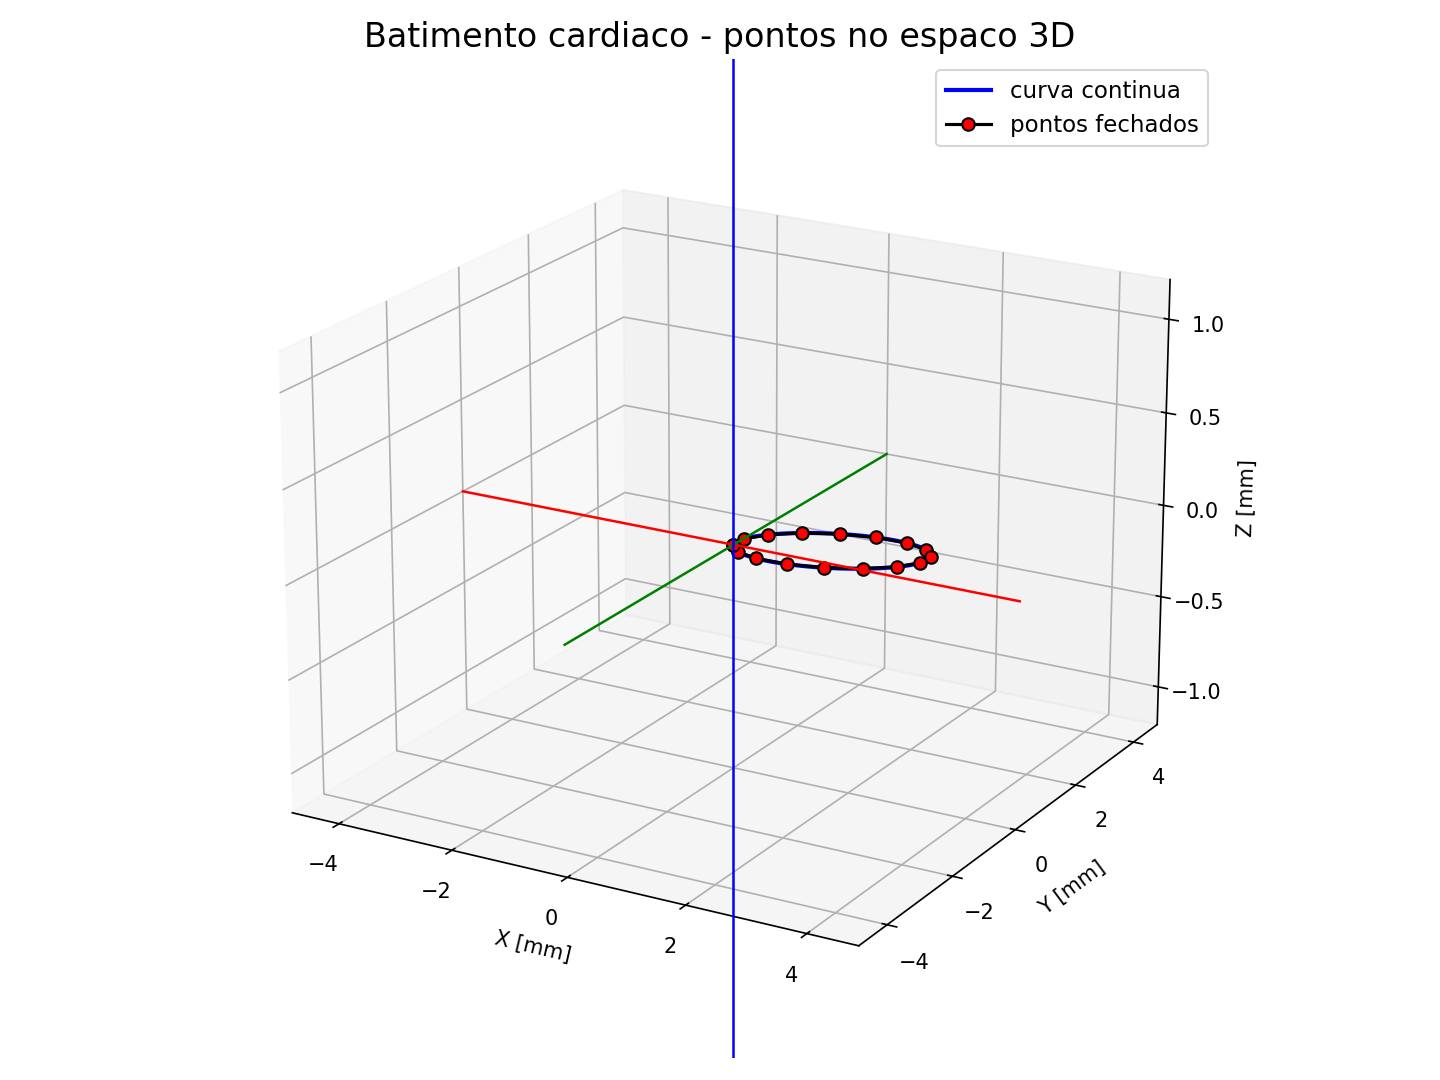
\includegraphics[width=0.62\textwidth]{movimentos/movimento_batimento_3d.png}
  \caption{Trajetória calculada para o movimento de batimento cardíaco, representação 3D dos pontos de passagem.}
  \label{fig:movimento-batimento-3d}
\end{figure}

Como explicado anteriormente, para a respiração foi utilizada a mesma parábola, no plano \(ZX\), de modo a captar o acoplamento entre a componente craniocaudal dominante e a ligeira componente lateral. Ao longo da curva, a coordenada \(Z\) cresce de forma acentuada, refletindo o deslocamento vertical imposto pelo diafragma, com variação lenta no início e mais acentuada no final do trajeto, enquanto a coordenada \(X\) avança de forma aproximadamente constante, traduzindo o deslizar lateral da árvore brônquica associado a esse movimento. A mesma curva é também usada como deslocamento rápido associado à tosse, alterando apenas o período de duração e o momento de ativação do evento. Dentro do cálculo da curva de respiração existe ainda uma componente de ajuste que permite configurar a inclinação do plano \(ZX\) em relação ao eixo \(X\), possibilitando orientar o deslocamento do movimento respiratório para um verdadeiro deslocamento crânio-caudal, caso necessário (por padrão, esta componente encontra-se neutra/desativada):
\begin{align}
  X_{3D}(u) &= u,\\
  Y_{3D}(u) &= \frac{H}{L^2}u^2\sin(\theta),\\
  Z_{3D}(u) &= \frac{H}{L^2}u^2\cos(\theta),
\end{align}
\[
\{0 \leq u \leq L\}
\]
o mesmo intervalo já usado na curva base. Por estar limitado a este intervalo, o parâmetro \(u\) nunca é negativo, pelo que nenhuma das três coordenadas assume valores negativos: todas partem de \(0\), em \(u=0\), e crescem até ao respetivo valor máximo, atingido em \(u=L\), sendo esse máximo igual a \(L\) para \(X_{3D}\) e igual a \(H\) para o conjunto de \(Y_{3D}\) e \(Z_{3D}\) (repartido entre as duas consoante o ângulo \(\theta\)). Nos valores usados nos testes, foram considerados \(H=20\,mm\), \(L=12\,mm\), \(N=10\) pontos, \(\theta=0^\circ\), um período \(T=4\,s\), pausa inicial de \(0,6\,s\), pausa final de \(0,1\,s\) e ponto inicial igual a 5, este último definido para iniciar a trajetória a partir de uma posição intermédia.

\begin{figure}[H]
  \centering
  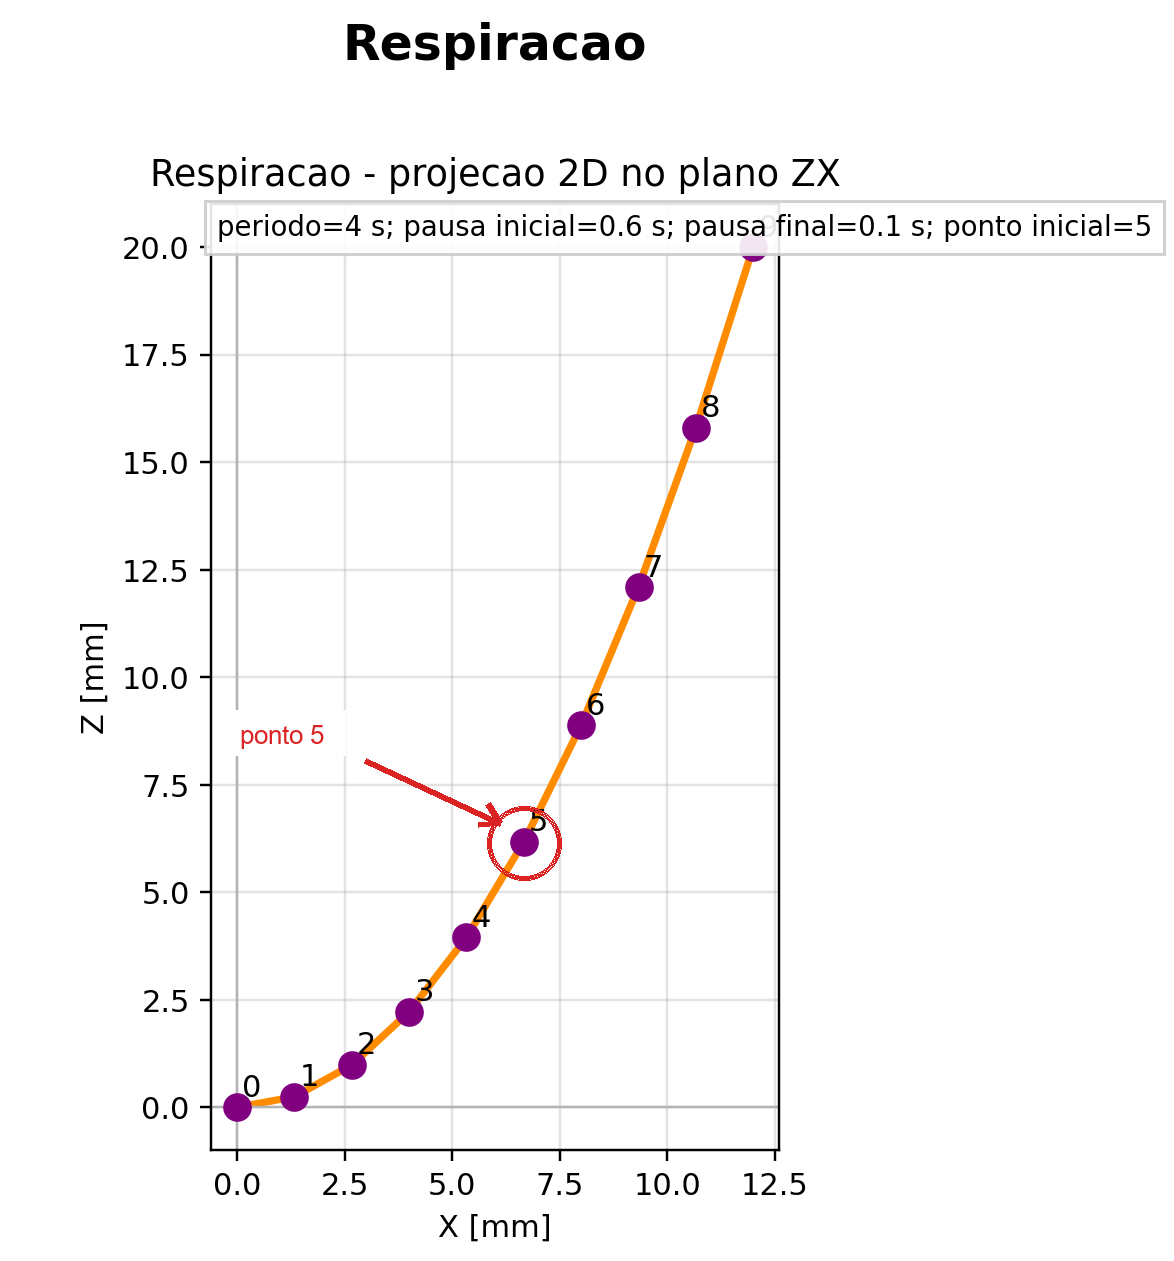
\includegraphics[width=0.62\textwidth]{movimentos/movimento_respiracao_2d.png}
  \caption{Trajetória calculada para o movimento respiratório, representação 2D no plano \(ZX\).}
  \label{fig:movimento-respiracao-2d}
\end{figure}

\begin{figure}[H]
  \centering
  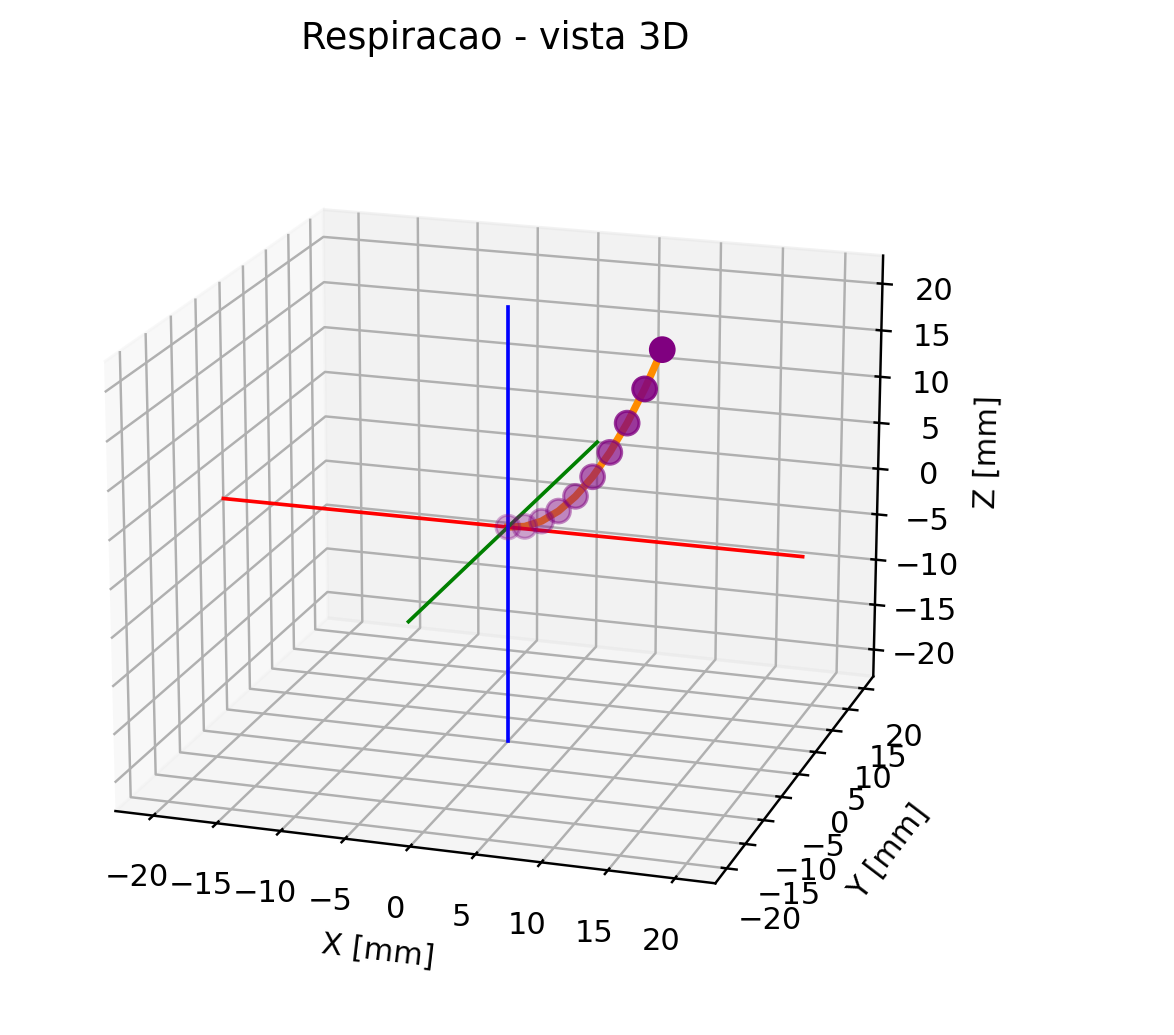
\includegraphics[width=0.62\textwidth]{movimentos/movimento_respiracao_3d.png}
  \caption{Trajetória calculada para o movimento respiratório, visualização 3D.}
  \label{fig:movimento-respiracao-3d}
\end{figure}

Além da alteração do movimento respiratório, a tosse inclui uma vibração curta em torno da posição de referência. Esta vibração foi representada, na sua forma base, por uma circunferência no plano \(XY\), sendo esta curva ainda modificada durante a execução no firmware do ESP32, de modo a produzir uma forma de vibração final com um comportamento mais irregular e aproximadamente aleatório:
\begin{align}
  X(u) &= r\cos(u),\\
  Y(u) &= r\sin(u),\\
  Z(u) &= 0.
\end{align}
O raio \(r\) controla a amplitude da vibração, o número de pontos controla a resolução da trajetória e o período define a rapidez do evento, tendo sido usado, no caso apresentado, \(r=2\,mm\), \(N=10\) pontos, sentido horário e período de \(0,5\,s\).

\begin{figure}[H]
  \centering
  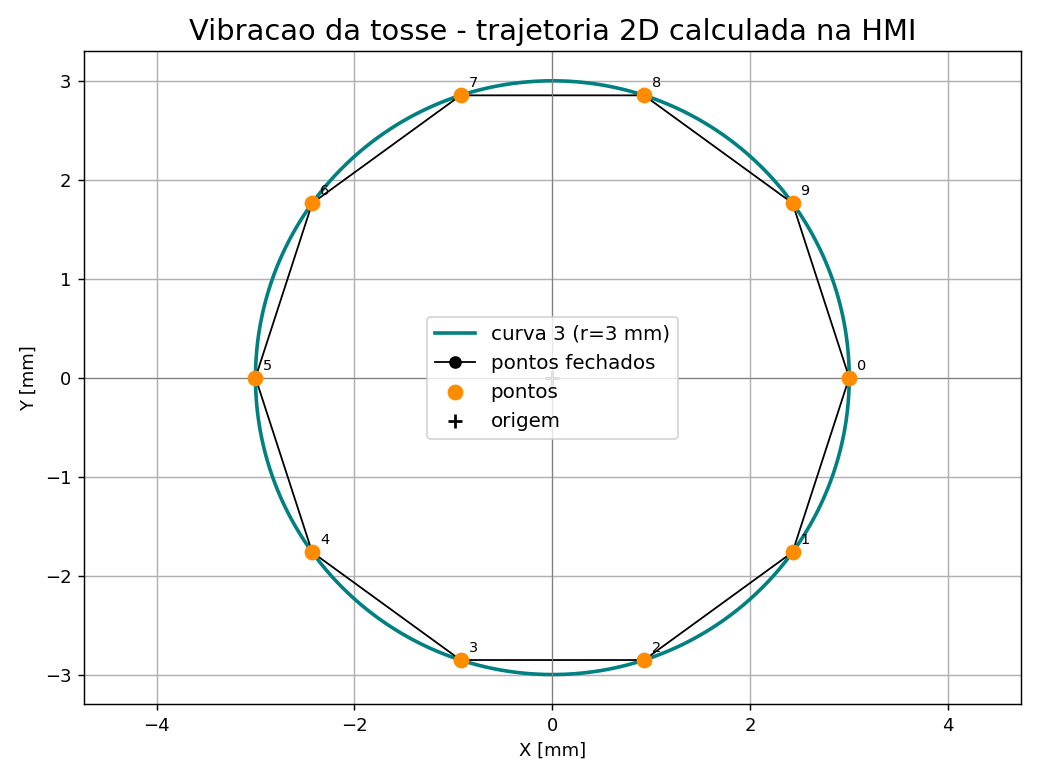
\includegraphics[width=0.62\textwidth]{movimentos/movimento_vibracao_tosse_2d.png}
  \caption{Trajetória calculada para a vibração associada à tosse, representação 2D dos pontos de passagem.}
  \label{fig:movimento-vibracao-tosse-2d}
\end{figure}

\begin{figure}[H]
  \centering
  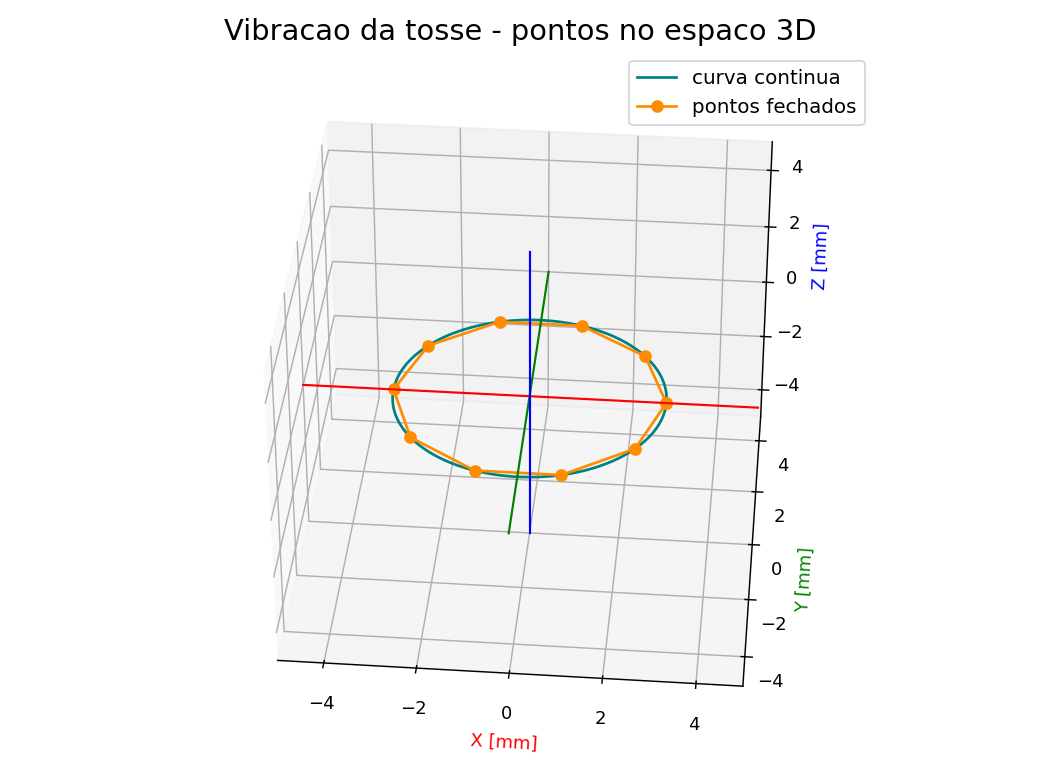
\includegraphics[width=0.62\textwidth]{movimentos/movimento_vibracao_tosse_3d.png}
  \caption{Trajetória calculada para a vibração associada à tosse, representação 3D dos pontos de passagem.}
  \label{fig:movimento-vibracao-tosse-3d}
\end{figure}

\begin{table}[H]
  \centering
  \caption{Parâmetros ajustáveis usados no cálculo dos movimentos na HMI.}
  \label{tab:parametros-calculo-movimentos}
  \small
  \begin{tabular}{p{3.0cm} p{5.7cm} p{5.3cm}}
    \toprule
    Movimento & Parâmetros geométricos & Parâmetros temporais e de execução\\
    \midrule
    Batimento cardíaco & \(a\), \(b\), \(R\), \(\alpha\), número de pontos e sentido da elipse & Período, pausa inicial, pausa final e ponto inicial\\
    Respiração & Altura \(H\), largura \(L\), ângulo \(\theta\) e número de pontos da parábola & Período, pausa inicial, pausa final, ponto inicial e modo bidirecional\\
    Vibração da tosse & Raio \(r\), número de pontos e sentido da circunferência & Período, pausa inicial, pausa final e ponto inicial\\
    \bottomrule
  \end{tabular}
\end{table}

Como o número de pontos é um parâmetro configurável em cada movimento, as trajetórias não precisam de ter obrigatoriamente a mesma discretização. A \cref{tab:pontos-calculados-movimentos} apresenta o conjunto de pontos usado no teste documentado, calculado diretamente pelo módulo Python da HMI, com 16 pontos para o batimento cardíaco e 10 pontos para os restantes dois movimentos (assinalados com um traço nas linhas em que não têm ponto correspondente).

\begin{table}[H]
  \centering
  \caption{Pontos calculados para os movimentos usados nos testes da interface.}
  \label{tab:pontos-calculados-movimentos}
  \scriptsize
  \setlength{\tabcolsep}{4pt}
  \resizebox{\textwidth}{!}{%
  \renewcommand{\arraystretch}{1.2}
  \begin{tabular}{c rrr rrr rrr}
    \toprule
    Ponto &
    \multicolumn{3}{c}{Batimento cardíaco} &
    \multicolumn{3}{c}{Respiração} &
    \multicolumn{3}{c}{Vibração da tosse}\\
    \cmidrule(lr){2-4}\cmidrule(lr){5-7}\cmidrule(lr){8-10}
    & \(X\) & \(Y\) & \(Z\) & \(X\) & \(Y\) & \(Z\) & \(X\) & \(Y\) & \(Z\)\\
    \midrule
    0  & 0,00 & 0,00  & 0,00 & 0,00  & 0,00 & 0,00  & 2,00  & 0,00  & 0,00\\
    \rowcolor{gray!8}
    1  & 0,01 & 0,31  & 0,00 & 1,33  & 0,00 & 0,25  & 1,62  & -1,18 & 0,00\\
    2  & 0,23 & 0,65  & 0,00 & 2,67  & 0,00 & 0,99  & 0,62  & -1,90 & 0,00\\
    \rowcolor{gray!8}
    3  & 0,63 & 0,97  & 0,00 & 4,00  & 0,00 & 2,22  & -0,62 & -1,90 & 0,00\\
    4  & 1,15 & 1,22  & 0,00 & 5,33  & 0,00 & 3,95  & -1,62 & -1,18 & 0,00\\
    \rowcolor{gray!8}
    5  & 1,71 & 1,36  & 0,00 & 6,67  & 0,00 & 6,17  & -2,00 & 0,00  & 0,00\\
    6  & 2,22 & 1,37  & 0,00 & 8,00  & 0,00 & 8,89  & -1,62 & 1,18  & 0,00\\
    \rowcolor{gray!8}
    7  & 2,61 & 1,26  & 0,00 & 9,33  & 0,00 & 12,10 & -0,62 & 1,90  & 0,00\\
    8  & 2,82 & 1,03  & 0,00 & 10,67 & 0,00 & 15,80 & 0,62  & 1,90  & 0,00\\
    \rowcolor{gray!8}
    9  & 2,81 & 0,72  & 0,00 & 12,00 & 0,00 & 20,00 & 1,62  & 1,18  & 0,00\\
    10 & 2,59 & 0,38  & 0,00 & --    & --   & --    & --    & --    & --\\
    \rowcolor{gray!8}
    11 & 2,19 & 0,06  & 0,00 & --    & --   & --    & --    & --    & --\\
    12 & 1,67 & -0,19 & 0,00 & --    & --   & --    & --    & --    & --\\
    \rowcolor{gray!8}
    13 & 1,11 & -0,33 & 0,00 & --    & --   & --    & --    & --    & --\\
    14 & 0,59 & -0,35 & 0,00 & --    & --   & --    & --    & --    & --\\
    \rowcolor{gray!8}
    15 & 0,21 & -0,23 & 0,00 & --    & --   & --    & --    & --    & --\\
    \bottomrule
  \end{tabular}}
\end{table}

\section{Estruturas de armazenamento de dados}
O funcionamento do firmware depende de um conjunto reduzido de estruturas que organizam a informação usada durante a execução. Esta organização foi importante para evitar que os parâmetros geométricos, os pontos de trajetória e o estado temporário das máquinas de estados ficassem dispersos pelo código principal, o que dificultaria tanto a calibração como a alteração posterior dos movimentos.

As estruturas mais importantes para o controlo dos manipuladores e para a execução das trajetórias começam pela \texttt{Manipulador\_Config}, resumida na \cref{fig:estrutura-manipulador-config} e concebida para concentrar toda a informação referente a cada manipulador Delta, tanto configurações como dados internos. Nela encontram-se definidos os comprimentos das várias ligações e dimensões do manipulador (\(L1\), \(L2\), \(L3\)), os deslocamentos associados à posição e à rotação global do manipulador, os limites mecânicos admissíveis, expressos em ângulos, os intervalos de PWM calibrados para cada servo, bem como variáveis internas de apoio ao próprio cálculo de IK. Assim, a cinemática inversa pode ser aplicada aos dois manipuladores a partir da mesma lógica matemática, mudando apenas os parâmetros específicos de montagem e calibração de cada conjunto.

\begin{figure}[!htbp]
  \centering
  \begin{tikzpicture}[
    hdr/.style={draw, thick, fill=blue!15, font=\small\bfseries\ttfamily,
                align=center, minimum width=6.4cm, minimum height=0.72cm},
    fld/.style={draw=gray!50, fill=white, font=\small\ttfamily,
                align=left, minimum width=6.4cm, minimum height=0.60cm, inner sep=4pt},
    fldout/.style={draw=gray!50, fill=green!8, font=\small\ttfamily,
                align=left, minimum width=6.4cm, minimum height=0.60cm, inner sep=4pt}
  ]
    \node[hdr]                    (mc0) at (0,0)    {Manipulador\_Config};
    \node[fld, below=0pt of mc0] (mc1)              {\quad L1,\ L2,\ L3};
    \node[fld, below=0pt of mc1] (mc2)              {\quad servoOffsetX,\ servoOffsetZ};
    \node[fld, below=0pt of mc2] (mc3)              {\quad angleMin,\ angleMax};
    \node[fld, below=0pt of mc3] (mc4)              {\quad rotationOffsetZ};
    \node[fld, below=0pt of mc4] (mc5)              {\quad servo1/2/3: MinPulse,\ MaxPulse};
    \node[fld, below=0pt of mc5] (mc6)              {\quad theta1/2/3: MinPulse,\ MaxPulse};
    \node[fldout, below=0pt of mc6] (mc7)           {\quad servo1/2/3Pulse\ \ \textit{(saída IK)}};
  \end{tikzpicture}
  \caption{Estrutura \texttt{Manipulador\_Config}, com os parâmetros de geometria, calibração de PWM e o estado atual dos pulsos gerados pela cinemática inversa.}
  \label{fig:estrutura-manipulador-config}
\end{figure}

O armazenamento da informação de cada movimento foi deliberadamente dividido em duas estruturas distintas, uma fixa e outra dinâmica, em vez de reunir tudo numa única estrutura. Esta separação torna o seu uso mais versátil, já que o sistema, sempre que precisa de modificar ou atualizar variáveis auxiliares associadas à execução de um movimento, não necessita de carregar uma estrutura completa com toda a informação, incluindo os arrays de pontos da trajetória, que em certos casos poderia representar um volume considerável de dados. Desta forma, o funcionamento do firmware fica otimizado, evitando sobrecarregar o código e sem comprometer o próprio cálculo das posições em tempo real.

A componente fixa desta divisão é a estrutura \texttt{MotionStorage}, que descreve a trajetória em si, através dos arrays de pontos \(X\), \(Y\) e \(Z\), do número de pontos, do período total, dos tempos de pausa no início e no fim, do ponto inicial e da indicação de o movimento ser, ou não, bidirecional. Estes dados correspondem à parte estática do movimento: definem o que deve ser executado, mas não dizem em que ponto da execução o sistema se encontra num dado instante.

A componente dinâmica, por sua vez, pertence à estrutura \texttt{MotionInstance}, que representa uma instância em funcionamento de uma trajetória guardada em \texttt{MotionStorage}. Em vez de duplicar os pontos do movimento, esta estrutura armazena a definição original sob a forma de um ponteiro, uma variável que não guarda os dados em si, mas apenas o endereço de memória onde a estrutura \texttt{MotionStorage} correspondente está alojada. Isto permite aceder à mesma trajetória a partir de uma única referência, sem necessidade de chamar as duas estruturas em separado, mantendo ao mesmo tempo a vantagem de as ter fisicamente separadas na memória. A \texttt{MotionInstance} guarda apenas o estado de execução: índices atuais, direção de avanço, temporizadores, multiplicador de amplitude em \(Z\), flags de ativação e estado atual da máquina de estados. Esta distinção entre definição e execução permite aplicar a mesma rotina genérica à respiração, ao batimento cardíaco e à vibração da tosse, mantendo cada movimento com o seu próprio estado interno. A \cref{fig:estruturas-motion} resume os campos destas duas estruturas e a ligação por ponteiro entre elas.

\begin{figure}[!htbp]
  \centering
  \resizebox{0.85\textwidth}{!}{%
  \begin{tikzpicture}[
    hdr/.style={draw, thick, fill=blue!15, font=\small\bfseries\ttfamily,
                align=center, minimum width=6.4cm, minimum height=0.72cm},
    fld/.style={draw=gray!50, fill=white, font=\small\ttfamily,
                align=left, minimum width=6.4cm, minimum height=0.60cm, inner sep=4pt},
    ptr/.style={-Latex, thick, dashed, blue!60!black}
  ]
    %% ── MotionStorage ──
    \node[hdr]                    (ms0) at (0,0)    {MotionStorage};
    \node[fld, below=0pt of ms0] (ms1)              {\quad X[],\ Y[],\ Z[]\ \ \textit{(trajetória)}};
    \node[fld, below=0pt of ms1] (ms2)              {\quad n\_Points,\ N\_points};
    \node[fld, below=0pt of ms2] (ms3)              {\quad start\_Index};
    \node[fld, below=0pt of ms3] (ms4)              {\quad period};
    \node[fld, below=0pt of ms4] (ms5)              {\quad bidirectional\ \ \textit{(bool)}};
    \node[fld, below=0pt of ms5] (ms6)              {\quad T\_pause\_Ini,\ T\_pause\_End};
    \node[fld, below=0pt of ms6] (ms7)              {\quad dtMs};
    \node[fld, below=0pt of ms7] (ms8)              {\quad Dt\_pauseMs\_Ini,\ Dt\_pauseMs\_End};

    %% ── MotionInstance ──
    \node[hdr]                    (mi0) at (7.6,0) {MotionInstance};
    \node[fld, below=0pt of mi0] (mi1)              {\quad *def\ $\to$\ MotionStorage};
    \node[fld, below=0pt of mi1] (mi2)              {\quad currentIndex,\ iIndex,\ jIndex};
    \node[fld, below=0pt of mi2] (mi3)              {\quad I\_Index,\ End\_Point};
    \node[fld, below=0pt of mi3] (mi4)              {\quad Direction\ \ (+1\,/\,$-$1)};
    \node[fld, below=0pt of mi4] (mi5)              {\quad segmentStartMs};
    \node[fld, below=0pt of mi5] (mi6)              {\quad elapsed\_1,\ elapsed\_2,\ elapsed\_3};
    \node[fld, below=0pt of mi6] (mi7)              {\quad Dt\_pause};
    \node[fld, below=0pt of mi7] (mi8)              {\quad Z\_amp\_mult};
    \node[fld, below=0pt of mi8] (mi9)              {\quad active,\ Executing};
    \node[fld, below=0pt of mi9] (mi10)             {\quad Individual\_start\_comand};
    \node[fld, below=0pt of mi10] (mi11)            {\quad state\ \ \textit{(FSM)},\ Situacion};

    %% ── ponteiro ──
    \draw[ptr] (mi1.west) -- ++(-0.5,0) |- (ms0.east);
  \end{tikzpicture}}
  \caption{Estruturas \texttt{MotionStorage} e \texttt{MotionInstance}, com a ligação por ponteiro entre a definição estática da trajetória e o estado dinâmico de execução.}
  \label{fig:estruturas-motion}
\end{figure}

Na prática, esta separação facilita também a sobreposição de movimentos: a respiração, o batimento cardíaco e a tosse são percorridos por três instâncias distintas, cada uma com a sua própria cadência, o que permite ativar temporariamente a perturbação da tosse sem alterar a definição base das restantes trajetórias. O resultado final de cada instante é obtido mais à frente, na etapa de fusão e cinemática inversa, mas a consistência desse cálculo depende desta estruturação prévia dos dados.

\section{Máquinas de estados e execução dos movimentos}
No ESP32, o firmware não tem como função principal desenhar ou recalcular as curvas geométricas dos movimentos, mas sim gerir a execução, em tempo real, dos pontos de trajetória já definidos e armazenados nas estruturas \texttt{MotionStorage}/\texttt{MotionInstance} apresentadas na secção anterior. É precisamente esta separação entre a definição estática da trajetória e o seu estado dinâmico de execução que permite aplicar a mesma máquina de estados à respiração, ao batimento cardíaco e à vibração da tosse, cada uma com a sua própria instância e cadência de funcionamento.

\subsection{Desenvolvimento e iterações}\label{subsec:desenvolvimento-execucao}
O mecanismo de execução aqui descrito, comum aos três movimentos, resultou de uma evolução por várias etapas, recorrendo-se (nas primeiras validações) apenas a um único movimento linear fixo e simples o suficiente para confirmar isoladamente o funcionamento da cinemática inversa, sem ainda qualquer preocupação com a forma final de comandar a respiração, o batimento cardíaco ou a tosse.

Nas fases iniciais de planeamento do sistema responsável por comandar estes movimentos, foram ponderadas diferentes abordagens, com resultados desiguais entre si. Contudo, uma decisão manteve-se presente desde o início: a utilização de máquinas de estados, de modo a garantir que todos os subsistemas do firmware pudessem funcionar em simultâneo sem bloquear a execução de outros comandos. A questão que se colocava não era, portanto, se usar máquinas de estados, mas sim como estruturar, através delas, o processo de execução dos movimentos.

Uma das primeiras ideias consideradas foi o envio em tempo real das coordenadas absolutas dos manipuladores, calculadas na HMI e transmitidas continuamente para o ESP32 à medida que fossem geradas. Esta abordagem foi abandonada pelas razões já discutidas a propósito da fusão de movimentos (\cref{sec:geracao-trajetorias}), agravadas por duas limitações adicionais: a comunicação série não ser suficientemente rápida para sustentar um fluxo contínuo de coordenadas ao ritmo exigido e a ausência de qualquer noção de tempo entre pontos, o que tornaria impossível suavizar a transição de um ponto para o seguinte, já que os motores tendem, por natureza, a atingir a posição seguinte o mais depressa possível. Este comportamento dos motores está diretamente relacionado com a natureza dos próprios servos, já descrita na \cref{sec:selecao-atuacao}: dispõem de um único canal de comunicação através do qual lhes é constantemente indicada a posição a atingir, cabendo ao seu controlador interno chegar lá o mais depressa possível, sem qualquer capacidade própria de regular a velocidade do movimento, uma limitação que o próprio mecanismo de interpolação descrito ao longo desta secção viria a contornar.

Por estes motivos, a alternativa ao envio em tempo real passou a ser, como já referido, o cálculo e a organização prévia dos pontos na HMI, seguidos do seu envio controlado e do armazenamento no ESP32 através das estruturas \texttt{MotionStorage}/\texttt{MotionInstance}.

Contudo, permanecia por resolver o problema de controlar o tempo ao longo de todo o ciclo do movimento, de forma a garantir que este se mantinha consistente, sem atrasos nem adiantamentos. Uma primeira ideia consistiu em associar a cada array de posições um segundo array com a duração até ao ponto seguinte, atualizado por um contador que acompanhava continuamente o tempo decorrido no processador. Esta solução permitia avançar corretamente ao longo da trajetória e terminar o ciclo no fim do array, mas não resolvia o problema por completo: o movimento resultante ficava marcado por saltos bruscos entre pontos, exatamente o que se pretendia evitar.

Seguiu-se uma fase de pesquisa de soluções para suavizar esta transição, tendo sido identificadas duas famílias de abordagens: fórmulas matemáticas que subdividiam o movimento em vários micropassos, como um polinómio cúbico capaz de gerar uma trajetória em S entre um ângulo inicial \(\theta_s\) e um ângulo final \(\theta_e\), ao longo de um tempo total \(T_F\), com velocidade nula em ambos os extremos,
\[
\theta(t) = \theta_s + a_2\,t^2 + a_3\,t^3, \qquad a_2 = \frac{3(\theta_e-\theta_s)}{T_F^2}, \qquad a_3 = \frac{-2(\theta_e-\theta_s)}{T_F^3},
\]
e bibliotecas de suavização de sinal, como a \textit{Ramp} ou a \textit{Easing}, que, a partir de um valor atual, de um valor futuro, de uma duração e de um perfil de onda escolhido, geravam uma saída suavizada capaz de atenuar paragens bruscas. No entanto, ambas revelaram limitações importantes. A subdivisão do movimento com gestão da onda de aceleração funcionava bem para um único motor, mas mostrou-se pouco versátil para escalar ao número de motores envolvidos neste projeto (entre seis a nove, em simultâneo). Já as bibliotecas de suavização não garantiam que o restante funcionamento do sistema, executado em paralelo, não fosse perturbado, uma vez que várias delas dependiam internamente da função \texttt{delay()}, incompatível com o resto do firmware. A isto acrescia a necessidade de manter entre quatro a cinco arrays por movimento (três para as coordenadas \(X\), \(Y\) e \(Z\), um para o tempo entre pontos e um para o tipo de suavização, já que se pretendia variar esse perfil ao longo do próprio ciclo), numa altura em que se acreditava ainda ser necessário duplicar cada movimento para os dois manipuladores, em vez de o tratar de forma genérica. Por estas razões, ambas as abordagens acabaram por ser descartadas, ainda que uma das bibliotecas consideradas, a \textit{Easing}, tenha voltado a ser testada numa versão posterior e mais avançada do sistema.

Com estas limitações identificadas, o sistema a desenvolver teria de cumprir dois requisitos: nunca recorrer à função \texttt{delay()} e reduzir ao mínimo o número de arrays necessários por movimento.

Um aspeto ainda não referido, mas decidido desde cedo, era que a geometria destes movimentos exigia zonas de andamento mais rápido e outras mais lento, de modo a transmitir a sensação de abrandamento junto de curvas e de aceleração nos troços mais retos, tornando o movimento tão natural quanto possível. Durante bastante tempo, admitiu-se que isso exigiria calcular um tempo próprio para cada ponto, de modo a preservar o período total pretendido no final do ciclo. Verificou-se, no entanto, que essa complexidade era desnecessária: atribuindo o mesmo intervalo de tempo a todos os pontos e variando, em vez disso, o espaçamento entre eles (mais próximos onde o movimento deveria ser mais lento, mais afastados onde deveria ser mais rápido), obtinha-se exatamente o mesmo efeito percecionado (\cref{fig:densidade-pontos-velocidade}). Bastava, assim, dividir o período total pelo número de pontos do movimento, partindo do princípio de que os pontos entregues já respeitavam essa distribuição não uniforme desde a sua geração na HMI (\cref{sec:geracao-trajetorias}). O sistema de atualização de pontos podia então ser tão simples como inicialmente imaginado: um contador e um comparador de tempo, avançando de instante a instante para a coordenada seguinte.

\begin{figure}[h]
  \centering
  \begin{tikzpicture}[pt/.style={circle, fill=blue!70!black, inner sep=1.6pt}]
    \node[pt] (p0) at (0,0)    {};
    \node[pt] (p1) at (3.2,0)  {};
    \node[pt] (p2) at (4.6,0)  {};
    \node[pt] (p3) at (5.4,0)  {};
    \node[pt] (p4) at (6.8,0)  {};
    \node[pt] (p5) at (10.0,0) {};
    \draw[thick, gray!60] (p0) -- (p1) -- (p2) -- (p3) -- (p4) -- (p5);
    \draw[-Latex, thick, red!70!black] ($(p0)+(0,-0.55)$) -- node[below, font=\scriptsize]{\(\Delta t\)} ($(p1)+(0,-0.55)$);
    \draw[-Latex, thick, red!70!black] ($(p1)+(0,-0.55)$) -- node[below, font=\scriptsize]{\(\Delta t\)} ($(p2)+(0,-0.55)$);
    \draw[-Latex, thick, red!70!black] ($(p2)+(0,-0.55)$) -- node[below, font=\scriptsize]{\(\Delta t\)} ($(p3)+(0,-0.55)$);
    \draw[-Latex, thick, red!70!black] ($(p3)+(0,-0.55)$) -- node[below, font=\scriptsize]{\(\Delta t\)} ($(p4)+(0,-0.55)$);
    \draw[-Latex, thick, red!70!black] ($(p4)+(0,-0.55)$) -- node[below, font=\scriptsize]{\(\Delta t\)} ($(p5)+(0,-0.55)$);
    \node[above=3pt of p0, font=\scriptsize] {troço reto};
    \node[above=3pt of p2, xshift=8pt, font=\scriptsize] {curva};
    \node[above=3pt of p5, font=\scriptsize] {troço reto};
  \end{tikzpicture}
  \caption{Andamento variável obtido apenas por densidade de pontos: o intervalo de tempo \(\Delta t\) entre pontos consecutivos mantém-se sempre igual, sendo o espaçamento espacial menor junto a curvas (andamento mais lento) e maior nos troços retos (andamento mais rápido).}
  \label{fig:densidade-pontos-velocidade}
\end{figure}

Testado este mecanismo, restava ainda o problema da suavização intermédia entre pontos consecutivos: apesar de os movimentos resultarem, por si só, relativamente suaves, continuava a ser necessário subdividi-los em várias secções, algo que o simples aumento do número de pontos não resolvia isoladamente. Colocou-se então uma nova questão de arquitetura: aplicar essa suavização antes ou depois da fusão dos vários movimentos numa única trajetória por manipulador. Suavizar depois da fusão permitiria fazê-lo apenas uma vez por manipulador, mas suavizar antes trazia uma vantagem decisiva: a fusão passava a ser calculada sempre a partir da posição real e atual de cada movimento, em vez de uma posição já alterada pela suavização, que poderia a qualquer momento distorcer o resultado da fusão e originar trajetos irregulares. Foi esta segunda opção a escolhida.

Para a suavização em si, adotou-se uma abordagem próxima da subdivisão em micropassos considerada inicialmente, mas sem os calcular todos antecipadamente: aproveitando o próprio contador de tempo já usado na atualização do movimento, calculava-se, a cada ciclo do processador, um ponto intermédio correspondente ao instante decorrido dentro do intervalo \(\Delta t\) esperado entre dois pontos consecutivos. A este processo dá-se o nome de interpolação linear (\textit{lerp}), detalhada mais adiante junto da função que a implementa.

Nos testes realizados a este mecanismo, um movimento de cada vez para simplificar, a estratégia revelou-se eficaz em frequências médias e altas. Em frequências mais baixas, porém, os motores continuavam a apresentar pequenas paragens percetíveis. Colocou-se a hipótese de a causa estar na transição entre pontos. Em alternativa à interpolação linear entre dois pontos (o atual \(P_i\) e o seguinte \(P_j\)), testou-se uma interpolação polinomial com três pontos (o atual, o seguinte e um ponto futuro adicional \(P_k\)), na expectativa de obter uma aproximação mais suave ao ponto intermédio, sem transições acentuadas entre segmentos (\cref{fig:interpolacao-linear-poli}):
\[
L(t) = (1-t)\,P_i + t\,P_j, \qquad Q(t) = (1-t)^2\,P_i + 2(1-t)t\,P_j + t^2\,P_k, \qquad t \in [0,1].
\]

\begin{figure}[h]
  \centering
  \begin{tikzpicture}[pt/.style={circle, fill=black, inner sep=1.5pt}]
    \node[pt, label=below:{\(P_i\)}] (a0) at (0,0) {};
    \node[pt, label=above:{\(P_j\)}] (a1) at (3,0.9) {};
    \draw[thick, blue!70!black] (a0) -- (a1);
    \node[font=\footnotesize] at (1.5,-0.9) {Linear (dois pontos)};

    \node[pt, label=below:{\(P_i\)}] (b0) at (6,0) {};
    \node[pt, label=above:{\(P_j\)}] (b1) at (7.6,1.3) {};
    \node[pt, label=below:{\(P_k\)}] (b2) at (9,0.4) {};
    \draw[thick, red!70!black] (b0) .. controls (b1) .. (b2);
    \node[font=\footnotesize] at (7.5,-0.9) {Polinomial (três pontos)};
  \end{tikzpicture}
  \caption{Comparação entre a interpolação linear e a interpolação polinomial testadas.}
  \label{fig:interpolacao-linear-poli}
\end{figure}

Por mais que este sistema e a sua variável de aproximação ao ponto intermédio fossem afinados, o resultado mantinha-se semelhante ao da interpolação linear, o que apontava para uma causa distinta. Confirmou-se, com o auxílio da leitura interna do sinal enviado ao servo, que o problema não era de software, mas mecânico: os servos utilizados tinham uma resolução por passo superior a \(1^\circ\). Em frequências mais baixas, isso exigia incrementos demasiado pequenos para que o servo os conseguisse traduzir num movimento real, resultando em saltos mais percetíveis do que em frequências mais altas. Não sendo viável substituir os motores nesta fase, optou-se por manter a solução de software e procurar mais tarde soluções mecânicas complementares, como amortecedores ou uma caixa redutora acoplada ao servo.

Identificada a causa dos saltos, voltou-se à interpolação linear, que apresentava resultados semelhantes aos da interpolação polinomial com menor complexidade e menos linhas de código. Esta foi, por isso, a interpolação efetivamente usada no código final, com o seu coeficiente saturado entre \(0\) e \(1\), tal como detalhado no módulo final desta secção. Esta saturação trouxe ainda uma vantagem adicional: caso a frequência de um movimento fosse extremamente alta e o intervalo \(\Delta t\) demasiado curto, o valor de saída nunca é comprometido por um passo desatualizado, atravessando o processo praticamente sem efeito.

Chegou-se assim à sequência final de processamento adotada (\cref{fig:pipeline-execucao}):

\begin{figure}[h]
  \centering
  \textbf{Atualização do movimento} \(\;\to\;\) \textbf{Suavização por interpolação linear} \(\;\to\;\) \textbf{Fusão dos movimentos}
  \caption{Sequência final de processamento, repetida a cada ciclo e para cada manipulador.}
  \label{fig:pipeline-execucao}
\end{figure}

Com este mecanismo testado e validado, a execução ainda apresentava uma limitação relevante: só aceitava trajetórias organizadas como ciclos fechados, sob pena de introduzir um salto acentuado entre secções mal ligadas. Era este o caso da respiração, testada até então com uma duplicação das suas coordenadas em sentido inverso, de modo a simular artificialmente um ciclo fechado.

A geometria da parábola escolhida para a respiração tornava difícil fechar o ciclo com limites suaves. Manter coordenadas duplicadas em sentidos opostos era, por si, pouco conveniente, sobretudo tendo em vista a futura integração da tosse, um evento de ocorrência imprevisível. Optou-se por isso por deixar este movimento aberto, o que exigiu acrescentar à execução a capacidade de percorrer certas trajetórias nos dois sentidos, para a frente e para trás. Para as trajetórias marcadas como bidirecionais, o ciclo passou a percorrer-se num sentido até ao último ponto e, de seguida, no sentido inverso até ao ponto inicial, com paragens configuráveis no fim de cada percurso quando aplicável. A gestão dos índices \(i\) e \(j\) junto destes extremos e das pausas é detalhada mais adiante nesta secção, a propósito da \cref{fig:fsm-motion}.

Uma última alteração a este sistema surgiu já na implementação da tosse, motivada pela necessidade de aumentar temporariamente a amplitude do movimento no momento da contração brônquica. Como todas as coordenadas geradas na HMI partem do ponto \((0,0)\) do respetivo plano, associado à posição de repouso do manipulador, multiplicar essa amplitude fazia crescer o ciclo apenas no sentido positivo do eixo \(Z\) e não de forma simétrica em torno do centro do movimento, como seria fisiologicamente esperado.

A solução passou por iniciar o ciclo num ponto intermédio da curva, em vez de num dos seus extremos, dividindo assim as coordenadas em duas partes, uma positiva acima desse ponto e outra negativa abaixo dele, com o próprio ponto de partida a assumir o papel do novo \((0,0)\) da curva. Para preservar a simplicidade do cálculo de pontos na HMI, esta alteração não foi introduzida na origem dos dados, mas sim diretamente no firmware: sempre que o índice inicial \texttt{start\_Index} é diferente de zero, a coordenada desse ponto é subtraída, em tempo real, à coordenada do ponto atual, permitindo escolher livremente qualquer ponto como início do ciclo sem alterar os dados armazenados. A única alteração estrutural necessária foi passar de duas para três sequências na atualização do movimento: do ponto inicial até ao último ponto, deste até ao ponto \(0\) e, por fim, do ponto \(0\) de volta ao ponto inicial. Esta forma de indexação trouxe ainda uma vantagem adicional: caso a tosse fosse acionada durante o avanço do ciclo, o sentido de atualização podia ser invertido de imediato, recuperando o sistema de forma natural a partir dessa nova direção.

\subsection{Módulo final}\label{subsec:modulo-final-execucao}
Nesta etapa final, todo o processo de gestão e execução do movimento consiste em percorrer os arrays de pontos já calculados e armazenados, avançar os índices ao ritmo certo e pela sequência correta, gerir eventuais pausas, traduzir esses índices em coordenadas reais e, por fim, unir os três movimentos numa só trajetória contínua e realista para cada manipulador. Esta sequência é executada por três mecanismos distintos: a \texttt{FSM\_Motion\_Update}, que gere os índices e a sequência dos ciclos, a função \texttt{Intermed\_position()}, que converte esses índices em coordenadas e calcula o ponto intermédio correspondente ao tempo decorrido, e por fim a função \texttt{Fusao\_plus\_IK\_D1}/\texttt{Fusao\_plus\_IK\_D2}, que une os três movimentos numa única saída para a cinemática inversa.

\paragraph{Primeira etapa: intervalo de tempo por segmento.}
O ritmo a que os índices avançam depende do intervalo \(\Delta t\) atribuído a cada segmento, calculado a partir do período total do movimento \(T\) e do número de pontos \(N\), considerando também a ida e o regresso nos movimentos bidirecionais:
\begin{equation}
  N_{\mathrm{seg}} =
  \begin{cases}
    2(N-1), & \text{movimento bidirecional},\\
    N-1, & \text{movimento não bidirecional},
  \end{cases}
  \qquad
  \Delta t = \frac{T}{N_{\mathrm{seg}}}.
\end{equation}

\paragraph{Segunda etapa: avanço dos índices.}
Os índices \(i\) e \(j\) (que representam, respetivamente, o ponto de partida e o ponto de chegada do segmento atual da trajetória) são avançados ao ritmo definido por \(\Delta t\) pela função genérica \texttt{FSM\_Motion\_Update}, capaz de percorrer qualquer trajetória associada a uma \texttt{MotionInstance}, independentemente do movimento em causa. A \cref{fig:fsm-motion} representa a sua sequência lógica, incluindo os estados principais, as pausas inicial e final, a inversão de direção e o tratamento do movimento bidirecional.

A \texttt{FSM\_Motion\_Update()} recebe, a cada ciclo de execução, o sinal global de arranque (\texttt{start}), a referência da instância de movimento (\texttt{inst} \(\rightarrow\) \texttt{MotionInstance}) e o instante de tempo atual (\texttt{nowMs}). Com estes dados, mantém atualizados os índices de trajetória e o cronómetro interno, sem calcular a posição em si, responsabilidade que pertence à terceira etapa.

\paragraph{Interação com as estruturas de dados.}
A cada chamada, a FSM lê os campos estáticos da \texttt{MotionStorage} associada (via \texttt{inst.def}) e atualiza os campos dinâmicos da \texttt{MotionInstance} correspondentes ao estado de execução, ambos já apresentados na \cref{fig:estruturas-motion}.

\clearpage
\begin{figure}[p]
  \centering
  \vspace*{-1.0cm}
  \resizebox{1.15\textwidth}{!}{%
  \begin{tikzpicture}[
    x=0.43cm,
    y=0.80cm,
    state/.style={draw, circle, align=center, minimum size=2.5cm, font=\small, thick, inner sep=3pt},
    arrow/.style={-Latex, thick},
    rlabel/.style={fill=white, inner sep=1pt},
    >=Stealth
  ]
    % �"?�"? Nome do estado a negrito no topo, variáveis abaixo �"?�"?
    \node[state, fill=blue!10]   (s0)  at (-12.0, 28) {{\large\textbf{S0}}\\[2pt]$I{=}0$\\$i{=}0$\\$j{=}0$\\$Exec{=}0$};
    \node[state, fill=blue!10]   (s1)  at (0.0, 26.5) {\textbf{S1}\\[2pt]$I{=}0$\\Situa\c{c}\~ao$=$P\\$j{=}1$};
    \node[state, fill=blue!10] (s2) at (15.5, 25.5) {\textbf{S2}\\[1pt]$Exec{=}1$\\$Inst.Segm{=}now$\\$i{=}P_{ini}$\\$j{=}i{+}d$\\$P_{fim}{=}m.nPts$};
    \node[state, fill=blue!10]   (s3)  at (4.0, 21.5) {\textbf{S3}\\[2pt]$T_{Decorrido1}{=}$\\$now{-}Inst.Segm$};
    \node[state, fill=blue!10] (s4) at (3.5, 13.0) {\textbf{S4}\\[1pt]$I{+}{+}$\\$i{=}i{+}d$\\$j{=}i{+}d$\\$Inst.Segm{=}now$};
    \node[state, fill=green!10]  (s13) at (22.0, 19.5) {\textbf{S13}\\[2pt]$Inst.Segm{=}now$};
    \node[state, fill=green!10]  (s14) at (14.0, 13.5)  {\textbf{S14}\\[1pt]$Signal{=}0$\\$d{=}{-}1$\\$P_{fim}{=}0$};
    \node[state, fill=green!10] (s11) at (14.0, 8.5) {\textbf{S11}\\[1pt]$i{=}m.Pts$\\$j{=}i{+}d$\\$P_{fim}{=}0$};
    \node[state, fill=green!10] (s12) at (23.0, 6.5) {\textbf{S12}\\[1pt]$i{=}0$\\$j{=}i{+}d$\\$P_{fim}{=}m.Pts$};
    \node[state, fill=orange!12] (s5)  at (3.0, 5.0) {\textbf{S5}\\[2pt]$Inst.Segm{=}now$\\$j{=}i$};
    \node[state, fill=orange!12] (s6)  at (15.0, 1.5)  {\textbf{S6}\\[2pt]$d{=}d\!\times\!({-}1)$};
    \node[state, fill=orange!12] (s7)  at (-9.5, 8.0) {\textbf{S7}\\[2pt]$DT_{pausa}$\\$=DT_{Pausa.ini}$};
    \node[state, fill=orange!12] (s8)  at (-13.0, 4.0)  {\textbf{S8}\\[2pt]$DT_{pausa}$\\$=DT_{Pausa.fim}$};
    \node[state, fill=orange!12] (s9)  at (-12.5, 14.8) {\textbf{S9}\\[2pt]$T_{Decorrido2}$\\${=}now{-}Inst.Segm$};
    \node[state, fill=gray!10]   (s10) at (-13.5, 21.0) {\textbf{S10}};

    % ?? Seta de in�cio ??
    \draw[arrow] (-10, 32.0) node[above]{\small INI} -- (s0.north);

    % ?? S0: loop e sa�da ??
    \draw[arrow] (s0) edge[loop, out=60, in=20, looseness=7] node[above right]{\small Start$=$0} (s0);
    \draw[arrow] (s0) -- (s1);

    % ?? S1: loop e retorno a S0 ??
    \draw[arrow] (s1) edge[loop above] node[above]{} (s1);
    \draw[arrow] (s1.west) to[out=-150, in=-60] node[rlabel, below, align=center]{\small M.Pts$\le$1\\M.Per$\le$0} (s0.south);

    % ?? S1 ? S2 ??
    \draw[arrow] (s1) -- node[rlabel, above, align=left]{\small $d{==}1$\\\& Sent$==$1} (s2);

    % ?? Cadeia principal S2?S3?S4 ??
    \draw[arrow] (s2) -- (s3);
    \draw[arrow] (s3.south east) to[out=-45, in=45] node[rlabel, pos=0.50, above, align=center]{\small $Elapsed_1\!\ge\!DT_{MS}$} (s4.north east);

    % ?? S4: retorno a S3 ??
    \draw[arrow] (s4.north west) to[out=120, in=-135] node[rlabel, pos=0.55, right, align=left]{\small $i{<}P_{fim}$ \& $d{=}1$\\$i{>}P_{fim}$ \& $d{=}{-}1$} (s3.south west);

    % ?? S4 ? S5 ??
    \draw[arrow] (s4.south) -- node[rlabel, right, align=left]{\small $i{\ge}P_{fim}$ \& $d{=}1$\\$i{\le}P_{fim}$ \& $d{=}{-}1$} (s5.north);

    % ?? S4 ? S14 ??
    \draw[arrow] (s4.east) -- (s14.west);

    % ?? S4 ? S1 ??
    \draw[arrow] (s4.west) to[out=150, in=-120] (s1.south);

    % ?? S5 ? S1 ??
    \draw[arrow] (s5.north west) to[out=140, in=-140] (s1.south);

    % ?? S13 ? S3 ??
    \draw[arrow] (s13.west) -- (s3.east);

    % ?? S14 ? S13 ??
    \draw[arrow] (s14.north east) to[out=45, in=-120] node[rlabel, right, align=left]{\small Signal$==$0\\\& Bidirecional} (s13.south west);

    % ?? S11 ? S13 / S12 ? S13 ??
    \draw[arrow] (s11.north east) to[out=45, in=-90] (s13.south);
    \draw[arrow] (s12.north) to[out=90, in=-60] (s13.south east);

    % ?? S5 ? S6 ??
    \draw[arrow] (s5) -- (s6);

    % ?? S6 ? S11 / S6 ? S12 ??
    \draw[arrow] (s6.north) to[out=90, in=-60] (s11.south);
    \draw[arrow] (s6.north east) to[out=60, in=-120] (s12.south);

    % ?? S5 para pausas ??
    \draw[arrow] (s5.west) to[out=165, in=-35] node[rlabel, pos=0.50, above, sloped]{\small pausa ini} (s7.south east);
    \draw[arrow] (s5.west) to[out=195, in=0] node[rlabel, pos=0.50, below, sloped]{\small pausa fim} (s8.east);

    % ?? S7 ? S9 ??
    \draw[arrow] (s7.north) to[out=135, in=-55] node[rlabel, pos=0.50, above, sloped]{\small medir} (s9.south east);

    % ?? S8 ? S9 ??
    \draw[arrow] (s8.north) to[out=110, in=-100] node[rlabel, pos=0.50, above, sloped]{\small medir} (s9.south);

    % ?? S9 ? S10 ??
    \draw[arrow] (s9) -- node[rlabel, pos=0.52, left, align=right]{\small $Elapsed_2{\ge}$\\$DT_{pausa}$} (s10);

    % ?? S10 ? S1 ??
    \draw[arrow] (s10.north east) to[out=25, in=-110] node[rlabel, pos=0.50, above]{\small Bidirecional$==$Falso} (s1.south west);
    \draw[arrow] (s10.south west)
        .. controls (-19.5, 14) and (-18, 8) .. (-18, 4)
        .. controls (-18, -1) and (5, -1) .. (s6.south west);
  \end{tikzpicture}}
  \caption{Esquema da FSM\_Motion\_Update.}
  \label{fig:fsm-motion}
\end{figure}

\clearpage

\paragraph{Fases de funcionamento.}
\begin{itemize}
  \item \textbf{Arranque (S0$\to$S1$\to$S2):} No estado S0, a instância encontra-se inativa, com os índices e a flag \texttt{Executing} a zero. Quando \texttt{start=1} e a instância está marcada como ativa, a FSM transita para S1, onde são validados os parâmetros da trajetória (pelo menos dois pontos e período positivo) e inicializado \texttt{Direction=1}. Em S2, regista-se \texttt{segmentStartMs=nowMs}, definem-se \texttt{iIndex=start\_Index} e \texttt{jIndex=iIndex+Direction}, transitando de imediato para S3.

  \item \textbf{Ciclo de segmentos (S3$\leftrightarrow$S4):} Em S3 mede-se o tempo decorrido (\texttt{elapsed\_1 = nowMs - segmentStartMs}), aguardando que este iguale \texttt{dtMs}. Atingido esse valor, S4 avança \texttt{iIndex} no sentido definido por \texttt{Direction} (\(+1\) ou \(-1\)), atualiza \texttt{jIndex=iIndex+Direction}, reinicia o cronómetro e regressa a S3. Este ciclo repete-se até \texttt{iIndex} atingir \texttt{End\_Point}.

  \item \textbf{Gestão do extremo e pausas (S5$\to$S7/S8$\to$S9$\to$S10):} Ao atingir o fim da passagem, S5 determina o percurso seguinte: existindo pausa configurada, S7 ou S8 carregam a duração correspondente (inicial ou final), S9 aguarda até esta terminar e S10 decide entre inverter o sentido e prosseguir o ciclo (\mbox{$\to$S6}) ou reiniciar do início (\mbox{$\to$S1}).

  \item \textbf{Inversão de direção (S6$\to$S11/S12$\to$S13):} Em S6, \texttt{Direction} é invertido (multiplicado por $-1$). Consoante o novo sentido, S11 (passagem descendente) ou S12 (passagem ascendente) reinicializa os índices no extremo correspondente. S13 regista o novo \texttt{segmentStartMs} e entra de imediato em S3.

  \item \textbf{Interrupção de tosse (S4$\to$S14$\to$S13):} Caso o sinal global \texttt{Tosse\_signal} seja ativado durante o avanço (S4), a FSM transita para S14, que força o sentido de regresso (\texttt{Direction=$-$1}, \texttt{End\_Point=0}) e encadeia de imediato com S13 para iniciar a descida de emergência.
\end{itemize}

\paragraph{Terceira etapa: cálculo da posição instantânea.}
Ao terminar cada chamada da FSM, a \texttt{MotionInstance} contém \texttt{iIndex} (índice do ponto de partida do segmento atual), \texttt{jIndex} (índice do ponto de chegada) e \texttt{elapsed\_1} (tempo decorrido desde o início do segmento). É este conjunto de valores que a função \texttt{Intermed\_position()} recebe, associando-lhes as coordenadas reais correspondentes: acede ao \texttt{MotionStorage} para obter \texttt{X[i]}, \texttt{X[j]}, \texttt{Y[i]}, \texttt{Y[j]}, \texttt{Z[i]}, \texttt{Z[j]} e o intervalo \texttt{dtMs} e calcula a posição interpolada entre os dois pontos, em função do tempo já decorrido no segmento. O resultado é um tripleto \((X,Y,Z)\) em coordenadas relativas ao ponto de referência \texttt{Index0}.

\begin{samepage}
A posição instantânea é obtida por interpolação linear entre dois pontos consecutivos da trajetória:
\[
  P(\alpha) = P_i + (P_j - P_i)\,\alpha
\]
Definindo a razão temporal bruta \(\alpha_0 = t_{dec}/DT_{MS}\), onde \(t_{dec}\) é o valor de \texttt{elapsed\_1} e \(DT_{MS}\) é \texttt{dtMs}, o coeficiente de interpolação saturado é:
\[
  \alpha = \begin{cases}
    0        & \text{se } \alpha_0 < 0 \\
    \alpha_0 & \text{se } 0 \le \alpha_0 \le 1 \\
    1        & \text{se } \alpha_0 > 1
  \end{cases}
  \qquad \alpha_0 = \frac{t_{dec}}{DT_{MS}}
\]
\end{samepage}

\paragraph{Quarta etapa: fusão das coordenadas.}
A função \texttt{Fusao\_plus\_IK\_D1}/\texttt{Fusao\_plus\_IK\_D2} combina as três coordenadas instantâneas (respiração, batimento e tosse) numa única coordenada por manipulador, somando a cada eixo um peso próprio por movimento e um deslocamento fixo específico do manipulador, de forma a posicionar corretamente a plataforma móvel dentro do espaço de trabalho de cada um. O resultado desta soma é entregue diretamente à função de cinemática inversa correspondente (\cref{sec:cinematica-inversa}), fechando a cadeia de execução tratada nesta secção.

\section{Preparação e sincronização da tosse}
A tosse é o único dos três movimentos representados que não corresponde a uma trajetória fisiológica contínua e previsível, mas sim a um evento pontual e imprevisível, sobreposto ao ciclo respiratório em curso. Esta secção descreve o mecanismo responsável por preparar e sincronizar esse evento com o movimento de respiração já em execução.

Esta funcionalidade foi implementada numa fase avançada do desenvolvimento, depois de os movimentos de respiração e batimento cardíaco já estarem validados de forma independente. Isso permitiu tratar a tosse como uma alteração temporária a um comportamento já existente, em vez de a construir de raiz.

A função de preparação da tosse é responsável por transformar um pedido de tosse num evento fisiológico sobreposto à respiração. Quando o sinal de tosse é ativado, a rotina guarda os parâmetros normais da respiração, reduz temporariamente o período, ajusta as pausas, aumenta a amplitude em \(Z\) e ativa, em paralelo, a instância de vibração ou perturbação da tosse.

Quando o ciclo respiratório atinge o estado apropriado para terminar o evento, a rotina repõe o período original, as pausas e o multiplicador de amplitude. Esta estratégia permite que a tosse não seja apenas uma trajetória independente, mas antes uma alteração temporária do comportamento respiratório, mais coerente com o fenómeno fisiológico que se pretende simular.

\section{Cinemática inversa do manipulador delta}\label{sec:cinematica-inversa}
A cinemática inversa é o algoritmo que converte a posição desejada da plataforma móvel \((X,Y,Z)\) num conjunto de ângulos, correspondendo cada um deles ao movimento que o respetivo atuador do manipulador tem de executar para que essa posição seja atingida. Os cálculos associados a esta conversão, num manipulador delta, são realizados inicialmente para um único braço, sendo depois repetidos de forma independente para os restantes, resultando nos três ângulos distintos \(\theta_1\), \(\theta_2\) e \(\theta_3\). Esta secção descreve, num primeiro momento, o percurso seguido até à abordagem final adotada e, de seguida, o algoritmo efetivamente implementado no firmware.

\subsection{Desenvolvimento e iterações}
O desenvolvimento deste cálculo começou por uma fase de pesquisa de trabalhos e repositórios já existentes sobre cinemática inversa para manipuladores delta. Embora existam bastantes artigos ou documentos académicos sobre o tema, a maioria dessas soluções recorria a matrizes de transformação relativamente complexas, cuja implementação direta em C++, num microcontrolador como o ESP32, revelava-se pouco prática e bastante complexa. Os repositórios que acabaram por inspirar o modelo final tinham em comum uma abordagem bem mais simples, assente em trigonometria simples e direta, com uma única matriz de rotação utilizada em todo o cálculo da cinemática inversa para atribuir as coordenadas e os ângulos de cada braço, o que tornava a sua implementação consideravelmente mais acessível.

A maioria destes trabalhos apresentava, no entanto, um problema comum: descreviam a cinemática de um manipulador delta na configuração mais habitual, a de um sistema \textit{pick-and-place}, montado com a plataforma voltada para baixo. Este projeto exigia precisamente o oposto, com a plataforma voltada para cima, de modo a poder ser acoplada ao modelo da árvore brônquica. A diferença pode parecer irrelevante, mas tem uma consequência prática: na orientação habitual, o antebraço do manipulador raramente ultrapassa o nível da base, pelo que o ângulo do atuador costuma ser descrito a partir do prolongamento de uma linha imaginária que liga o exterior do manipulador ao centro da base, cobrindo apenas \(180^\circ\) de amplitude no sentido positivo, com o restante percurso possível representado no sentido negativo (\cref{fig:convencao-angulo-horizonte}). Era o caso, por exemplo, da \textit{Delta-Kinematics-Library} \parencite{TinkersProjects2018} e da publicação de Nikanorov \parencite{Nikanorov_HyperTriangle}. Para este projeto, que exigia uma resolução angular mais fina do atuador de modo a permitir compactar ao máximo o sistema, esta convenção obrigaria a separar ângulos positivos e negativos em torno desse horizonte de referência, o que por sua vez exigiria recorrer a transformações adicionais e introduziria uma complexidade evitável.

\begin{figure}[htbp]
  \centering
  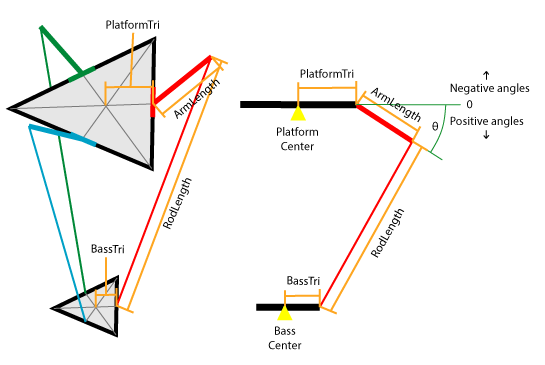
\includegraphics[width=0.75\textwidth]{figuras/convencao_angulo_delta_kinematics_library.png}
  \caption{Convenção de ângulo referenciada ao horizonte exterior do manipulador, usada na \textit{Delta-Kinematics-Library} \parencite{TinkersProjects2018}: a amplitude positiva fica limitada a \(180^\circ\) abaixo desse horizonte, com o restante percurso representado no sentido negativo.}
  \label{fig:convencao-angulo-horizonte}
\end{figure}

Uma solução mais adequada surgiu com o repositório de código aberto \textit{Delta-Robot}, de isaac879 \parencite{Isaac2019Delta}, que reformulava por completo o cálculo do ângulo do atuador: em vez de o referenciar ao horizonte exterior do manipulador, media-o a partir do centro da própria base, descrevendo uma rotação contínua de até \(360^\circ\) em torno desse centro, sem qualquer separação entre valores positivos e negativos. O repositório incluía ainda verificações de segurança que impediam o manipulador de atingir posições perigosas ou geometricamente impossíveis, assim como parâmetros de ajuste fino para a base, a plataforma, as uniões e os próprios atuadores, permitindo obter um resultado mais preciso do que os métodos anteriores. Continha, por fim, um método de conversão do ângulo calculado para o comando de um motor de posição genérico, bastando calibrar os seus limites em função do motor utilizado, assumindo um intervalo de rotação de \(180^\circ\), comum em servos, medido entre \(45^\circ\) e \(225^\circ\) a partir do centro da base, uma resolução de movimento mais próxima da habitualmente esperada para este tipo de manipulador.

Este repositório não pôde, no entanto, ser incorporado diretamente no firmware, tendo sido necessário adaptá-lo às necessidades do projeto. Foram removidos dois mecanismos, que não se enquadravam na filosofia do projeto: o sistema de coordenadas que subdividia internamente o movimento em vários micropassos, redundante face ao mecanismo de suavização por interpolação linear entretanto adotado (\cref{subsec:desenvolvimento-execucao}) e o sistema que permitia reorientar livremente o manipulador, desnecessário numa montagem de orientação fixa como a deste projeto. Em contrapartida, foram acrescentados a rotação global de cada manipulador, combinada com a rotação individual de cada braço já existente, bem como um ajuste à conversão final do ângulo, de modo a produzir diretamente o sinal PWM aceite pelos servos MG90S. A função de cinemática inversa foi ainda generalizada para aceitar qualquer configuração de manipulador, evitando duplicar código entre os dois manipuladores do sistema, seguindo a mesma lógica de generalização já aplicada à máquina de estados de execução dos movimentos.

Do lado dos motores, foi ainda necessário calibrar os limites do período de PWM, de modo a fazer corresponder o intervalo de \(45^\circ\) a \(225^\circ\) da cinemática inversa à amplitude de rotação física de cada servo, um procedimento detalhado no módulo final desta secção.

\subsection{Módulo final}
O algoritmo de cinemática inversa aqui descrito é executado, em cada ciclo do firmware, de forma independente para os três braços de cada manipulador, devolvendo o conjunto de ângulos para os atuadores, referente à posição pretendida da plataforma móvel. A \cref{fig:delta-cinematica-lateral} mostra a representação lateral usada como referência para as variáveis do cálculo: \(L_1\) representa o ante-braço acionado pelo servo, \(L_2\) o braço passivo, \(L_3\) a distância horizontal até à junta esférica da plataforma móvel, \(\phi\) e \(\omega\) são os ângulos intermédios calculados para cada braço e \(\theta\) é o ângulo final aplicado ao servo.

\begin{figure}[htbp]
  \centering
  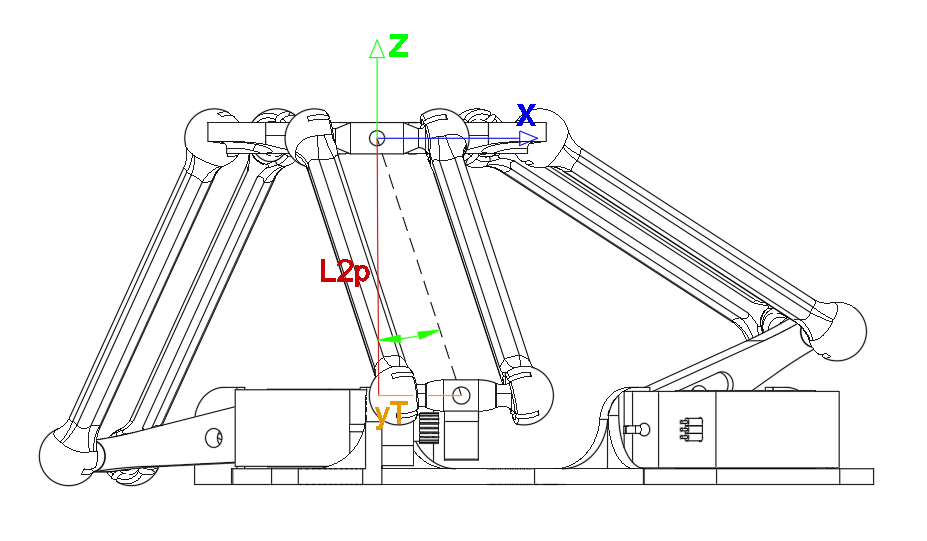
\includegraphics[width=0.82\textwidth]{figuras/Imagem lateral do Manipulador Delta.png}
  \caption{Representação lateral das variáveis usadas na cinemática inversa do manipulador delta.}
  \label{fig:delta-cinematica-lateral}
\end{figure}

O firmware aplica o mesmo cálculo aos três braços, distinguindo-os apenas pela rotação do referencial no plano \(XY\). Para cada manipulador existe um offset global \(\alpha_m\) (definido na estrutura \texttt{Manipulador\_Config}) e para cada servo existe uma rotação adicional \(\beta_k\):
\[
  \alpha_m =
  \begin{cases}
    -15^\circ, & \text{Manipulador Delta 1}\\
    -45^\circ, & \text{Manipulador Delta 2}
  \end{cases}
  \qquad
  \beta_k \in \{0^\circ,\;120^\circ,\;240^\circ\}
\]
\[
  \psi_k = \alpha_m + \beta_k
  \qquad
  R_z(\psi_k)=
  \begin{bmatrix}
    \cos\psi_k & -\sin\psi_k & 0\\
    \sin\psi_k &  \cos\psi_k & 0\\
    0             &  0             & 1
  \end{bmatrix}
\]
Assim, o ponto pedido é primeiro expresso no plano de trabalho do servo \(k\):
\[
  \begin{bmatrix}
    x'_k\\ y'_k\\ z'_k
  \end{bmatrix}
  =
  R_z(\psi_k)
  \begin{bmatrix}
    X\\Y\\Z
  \end{bmatrix}
  -
  \begin{bmatrix}
    0\\0\\z_{offset}
  \end{bmatrix}
  \quad
  \Longrightarrow
  \quad
  \begin{cases}
    x'_k = X\cos\psi_k - Y\sin\psi_k\\
    y'_k = X\sin\psi_k + Y\cos\psi_k\\
    z'_k = Z - z_{offset}
  \end{cases}
\]
(No firmware, o \(z_{offset}\), definido pela constante \texttt{SERVO\_OFFSET\_Z}, representa um ajuste fino à distância entre a base real do manipulador e a base onde os atuadores estão acoplados. Por omissão, este ajuste mantém-se a \(0\,\text{mm}\), uma vez que afeta apenas a forma como as coordenadas são referenciadas, podendo estas ser expressas diretamente a partir da base do atuador ou da base real do modelo físico.)

Após esta rotação, o problema passa a ser resolvido inteiramente no plano lateral do servo, correspondente à representação bidimensional da \cref{fig:delta-cinematica-lateral}. Nesse plano, a extremidade associada à plataforma móvel é deslocada pelo comprimento \(L_3\):
\[
  x_{arm,k}=x'_k+L_3
\]
O braço passivo \(L_2\) nem sempre se mantém contido no plano lateral do servo, uma vez que a plataforma móvel se pode deslocar lateralmente (eixo \(Y\)). O firmware compensa este desvio calculando o comprimento efetivo de \(L_2\) projetado nesse plano, sendo esta projeção apenas válida se a junta esférica da plataforma móvel não ultrapassar o limite angular admitido:
\[
  L_{2p,k}=\sqrt{L_2^2-y_k'^2}
  \qquad
  \gamma_k=\arcsin\!\left(\frac{y'_k}{L_2}\right)
  \qquad
  |\gamma_k| < 0{,}5934\,\text{rad}\approx34^\circ
\]
Este limite aparece no firmware como proteção para evitar que o ângulo entre a junta esférica e o braço passivo saia da zona mecânica admissível.

De seguida calcula-se a distância entre o eixo do servo e a projeção da junta esférica no plano lateral. Esta distância é designada no código por \texttt{ext}:
\[
  d_k=\sqrt{z_k'^2+\left(d_s-x_{arm,k}\right)^2}
  \qquad
  d_s=31{,}797\,\text{mm}
\]
onde \(d_s\), designado no código por \texttt{SERVO\_OFFSET\_X}, é a distância horizontal fixa, definida no desenho mecânico, entre o eixo do servo e a origem do referencial lateral.

Antes de calcular o ângulo, o firmware confirma se os comprimentos \(L_1\), \(L_{2p,k}\) e \(d_k\) conseguem formar um triângulo:
\[
  L_{2p,k}-L_1 < d_k < L_1+L_{2p,k}
\]
Se esta condição falhar, a posição pretendida fica fora do alcance geométrico daquele braço e a função de cinemática inversa devolve erro.

Com a geometria validada, o ângulo interno \(\phi_k\) é obtido pela lei dos cossenos, enquanto \(\omega_k\) corresponde à inclinação da reta entre o eixo do servo e a projeção da junta esférica:
\[
  \phi_k=
  \arccos\!\left(
    \frac{L_1^2+d_k^2-L_{2p,k}^2}{2L_1d_k}
  \right)
  \qquad
  \omega_k=
  \operatorname{atan2}\!\left(z'_k,\;d_s-x_{arm,k}\right)
\]
O ângulo enviado ao servo é então:
\[
  \theta_k=\phi_k+\omega_k
  \qquad
  45^\circ \le \theta_k \le 225^\circ
\]
O intervalo de \(45^\circ\) a \(225^\circ\) é o limite angular definido no firmware por \texttt{SERVO\_ANGLE\_MIN} e \texttt{SERVO\_ANGLE\_MAX}, pelo que, se algum dos três ângulos calculados ficar fora deste intervalo, a posição é rejeitada e os servos não são atualizados.

Por fim, cada \(\theta_k\) é convertido para largura de pulso PWM através do mesmo princípio de interpolação linear já utilizado para calcular a posição instantânea (\cref{subsec:modulo-final-execucao}), aplicado agora entre os limites de pulso mínimo e máximo do servo:
\[
  PWM_k =
  PWM_{k,min}+
  \frac{\theta_k-\theta_{min}}{\theta_{max}-\theta_{min}}
  \left(PWM_{k,max}-PWM_{k,min}\right)
\]
Considerando os valores de referência \(PWM_{min}=500\,\mu s\) e \(PWM_{max}=2500\,\mu s\), a relação é crescente no Manipulador Delta 1 e invertida no Manipulador Delta 2. Esta inversão decorre da montagem em espelho adotada para os dois manipuladores, que permite compactar o conjunto mas deixa o segundo manipulador fisicamente invertido em relação ao primeiro, obrigando a inverter também o sentido da correspondência entre ângulo e sinal PWM para obter o mesmo resultado final de movimento. Esta inversão é feita no arranque do firmware, quando os limites \texttt{thetaMinPulse} e \texttt{thetaMaxPulse} do segundo manipulador são trocados.

\begin{figure}[htbp]
  \centering
  \resizebox{\textwidth}{!}{%
  \begin{tikzpicture}[
    x=0.035cm,
    y=0.0026cm,
    axis/.style={->, thick},
    curve/.style={thick, blue!70!black},
    invcurve/.style={thick, orange!80!black},
    guide/.style={dashed, gray!60},
    lab/.style={font=\small},
    tick/.style={font=\scriptsize}
  ]
    % Delta 1
    \begin{scope}
      \draw[axis] (35,0) -- (238,0) node[lab, below right] {\(\theta_k\) [graus]};
      \draw[axis] (45,380) -- (45,2720) node[lab, above] {PWM [\(\mu s\)]};
      \draw[guide] (45,500) -- (225,500);
      \draw[guide] (45,2500) -- (225,2500);
      \draw[guide] (45,500) -- (45,0);
      \draw[guide] (225,2500) -- (225,0);
      \draw[curve] (45,500) -- (225,2500);
      \fill[curve] (45,500) circle (2.5pt);
      \fill[curve] (225,2500) circle (2.5pt);
      \node[lab, align=center] at (135,2860) {Manipulador Delta 1};
      \node[tick, below] at (45,0) {\(45^\circ\)};
      \node[tick, below] at (225,0) {\(225^\circ\)};
      \node[tick, left] at (45,500) {\(500\)};
      \node[tick, left] at (45,2500) {\(2500\)};
      \node[tick, above left] at (45,500) {min};
      \node[tick, above right] at (225,2500) {max};
    \end{scope}

    % Delta 2
    \begin{scope}[xshift=9.2cm]
      \draw[axis] (35,0) -- (238,0) node[lab, below right] {\(\theta_k\) [graus]};
      \draw[axis] (45,380) -- (45,2720) node[lab, above] {PWM [\(\mu s\)]};
      \draw[guide] (45,500) -- (225,500);
      \draw[guide] (45,2500) -- (225,2500);
      \draw[guide] (45,2500) -- (45,0);
      \draw[guide] (225,500) -- (225,0);
      \draw[invcurve] (45,2500) -- (225,500);
      \fill[invcurve] (45,2500) circle (2.5pt);
      \fill[invcurve] (225,500) circle (2.5pt);
      \node[lab, align=center] at (135,2860) {Manipulador Delta 2};
      \node[tick, below] at (45,0) {\(45^\circ\)};
      \node[tick, below] at (225,0) {\(225^\circ\)};
      \node[tick, left] at (45,500) {\(500\)};
      \node[tick, left] at (45,2500) {\(2500\)};
      \node[tick, above right] at (45,2500) {max};
      \node[tick, above left] at (225,500) {min};
    \end{scope}
  \end{tikzpicture}
  }
  \caption{Relação linear de referência entre o ângulo calculado pela cinemática inversa e o pulso PWM aplicado aos servos nos dois manipuladores.}
  \label{fig:pwm-servo-delta}
\end{figure}

Os limites de PWM usados no código não foram assumidos apenas a partir de valores teóricos do servo. Estes valores foram calibrados, começando pelo alinhamento da patilha de cada servo com a base onde estava acoplado. O objetivo deste alinhamento consistia em garantir que as posições físicas de \(0^\circ\) e \(180^\circ\) permaneciam paralelas em relação à superfície da base. Depois desse alinhamento mecânico, era feita a transição manual da referência física para o intervalo usado pela cinemática, mantendo-se o mesmo intervalo do período de PWM já calibrado. No Manipulador Delta 1, o \(0^\circ\) físico passava a corresponder ao \(45^\circ\) cinemático e o \(180^\circ\) físico ao \(225^\circ\) cinemático. No Manipulador Delta 2, devido à orientação oposta dos servos, o \(180^\circ\) físico passava a corresponder ao \(45^\circ\) cinemático e o \(0^\circ\) físico ao \(225^\circ\) cinemático. Por fim, foi necessário repetir ensaios de calibração para confirmar que os impulsos PWM correspondiam aos limites de \(45^\circ\) e \(225^\circ\), admitindo uma tolerância aproximada de \(\pm 5^\circ\).

\[
\text{Manipulador Delta 1 (calibrado):}
\left\{
\begin{array}{lcc}
& \text{Mínimo} & \text{Máximo}\\
\text{Servo } \theta_1: & 520\,\mu s & 2520\,\mu s\\
\text{Servo } \theta_2: & 550\,\mu s & 2550\,\mu s\\
\text{Servo } \theta_3: & 560\,\mu s & 2560\,\mu s
\end{array}
\right.
\]

\[
\text{Manipulador Delta 2 (calibrado):}
\left\{
\begin{array}{lcc}
& \text{Mínimo} & \text{Máximo}\\
\text{Servo } \theta_1: & 460\,\mu s & 2460\,\mu s\\
\text{Servo } \theta_2: & 470\,\mu s & 2470\,\mu s\\
\text{Servo } \theta_3: & 420\,\mu s & 2420\,\mu s
\end{array}
\right.
\]

Estes são os intervalos físicos efetivamente usados pelo firmware para associar cada servo ao seu canal PWM, já com a troca entre \texttt{thetaMinPulse} e \texttt{thetaMaxPulse} do Manipulador Delta 2 refletida nos valores calibrados acima. Note-se que, apesar de os valores absolutos diferirem ligeiramente entre servos, a largura bruta do intervalo mantém-se sempre em \(2000\,\mu s\), a mesma definida entre os valores de referência \(PWM_{min}=500\,\mu s\) e \(PWM_{max}=2500\,\mu s\) do datasheet, estando cada intervalo apenas deslocado em relação a essa referência. Isto garante que todos os servos percorrem o mesmo espaço angular, independentemente de os seus limites individuais estarem ligeiramente adiantados ou atrasados face ao valor teórico. Assim, a cinemática inversa gera sempre os mesmos três ângulos lógicos, independentemente do manipulador, cabendo apenas à conversão final para PWM refletir a montagem, o sentido de rotação e a calibração individual de cada servo.

\section{Comunicação série}
A comunicação entre o Raspberry Pi e o ESP32 assenta numa ligação série simples. O tratamento dessa ligação evoluiu, no entanto, de forma distinta em cada lado. No firmware, a comunicação é organizada por duas máquinas de estados dedicadas à receção e interpretação dos comandos, descritas na secção seguinte. No Raspberry Pi, assenta antes numa arquitetura de threads e filas que impede a interface de ficar bloqueada à espera da porta série, descrita mais adiante neste capítulo.

\subsection{Comunicação série no firmware (ESP32)}
A comunicação série encontra-se organizada em duas máquinas de estados distintas, cada uma responsável por uma função bem definida: a \texttt{FSM\_Serial\_reader()}, que trata apenas da receção dos dados entregues pela porta série, e a \texttt{FSM\_Serial\_Command()}, que interpreta esses dados de forma ordenada e altera o comportamento do sistema, bem como as suas configurações e dados internos. Esta separação evita que o resto do sistema fique sobrecarregado com a execução e o tratamento da informação inerentes à lógica de controlo dos movimentos.

\subsubsection{Desenvolvimento e iterações}
A primeira versão desta separação em duas máquinas de estados ficou operacional numa fase intermédia do projeto, com a \texttt{FSM\_Serial\_reader()} a manter-se, desde então, praticamente inalterada, sujeita apenas a pequenas correções pontuais ao longo do desenvolvimento. Foi sobretudo a \texttt{FSM\_Serial\_Command()} que sofreu sucessivas reformulações, à medida que o conjunto de comandos acompanhava o crescimento da interface gráfica do Raspberry Pi.

A primeira versão interpretava apenas caracteres isolados, associando cada um a uma ação fixa. Seguiu-se a introdução de um sistema de menus assente na mesma lógica de caracteres isolados, em que uma única letra passou a dar acesso a um conjunto de opções adicionais, também elas identificadas por um único carácter. A alteração mais significativa foi, no entanto, a introdução do modo de comandos por cadeia de caracteres, destinado a modificar diretamente valores inteiros ou fracionários das variáveis de movimento. Cada mensagem deste tipo precisava de indicar três coisas: que se tratava de uma escrita, a qual das três estruturas de movimento se destinava e a que variável interna dessa estrutura. Seguia-se a conversão do excerto numérico da cadeia para o respetivo valor, repetida tantas vezes quantas as necessárias nos campos que correspondem a arrays de pontos.

A primeira implementação deste modo resolvia o problema de forma simples, mas excessivamente extensa, exigindo cerca de vinte estados só para alterar uma única variável, de cada vez, em qualquer um dos movimentos. Na iteração mais recente, esta parte da máquina foi reconstruída de raiz com recurso a ponteiros, tanto para selecionar a estrutura de movimento visada como a variável interna a alterar, aproveitando o facto de as três estruturas de movimento partilharem sempre o mesmo conjunto de campos. Esta generalização permitiu manter o mesmo número de estados usado anteriormente para alterar uma única variável, cobrindo agora as oito variáveis internas disponíveis nas três estruturas de movimento.

\subsubsection{Módulo final}
A \texttt{FSM\_Serial\_reader()} funciona como uma camada de aquisição, representada na \cref{fig:fsm-serial-reader}. Consoante o modo ativo, lê da porta série um único carácter (modo simples) ou uma cadeia de caracteres até ao fim da mensagem (modo de comandos por cadeia), disponibilizando o resultado numa variável de saída própria e ativando, só depois de a leitura estar completa, uma flag de linha pronta. Assim, a máquina de comandos nunca precisa de ler diretamente da porta série, consumindo sempre comandos já preparados.

\begin{figure}[H]
  \centering
  \resizebox{0.98\textwidth}{!}{%
  \begin{tikzpicture}[
    state/.style={draw, circle, align=center, minimum size=1.8cm, font=\scriptsize, thick},
    arrow/.style={-Latex, thick},
    loopback/.style={-Latex, thick, blue!55!black},
    lab/.style={font=\tiny, fill=white, inner sep=1pt},
    >=Stealth
  ]
    \node[draw, rounded corners=2pt, align=left, font=\scriptsize, fill=white, inner sep=4pt]
      at (9.3,17.7) {M $\to$ modo múltiplo\\S $\to$ modo simples};

    \node[state, fill=blue!8]  (r0) at (3.5,17.0)  {0\\INIT\\contador=0};
    \node[state]               (r1) at (5.3,15.2)  {1\\CH\_Bus\\=Serial.read()};
    \node[state, fill=gray!12] (r4) at (8.5,16.3)   {4\\CH\_Bus\\=\textbackslash 0};
    \node[state, fill=orange!10](r2) at (5.3,12.6)  {2\\CH\_Command\\=CH\_Bus};
    \node[state, fill=gray!12] (r3) at (3.8,10.2)   {3\\CH\_Bus\\=\textbackslash 0};
    \node[state, fill=gray!12] (r5) at (6.8,10.2)   {5\\CH\_Bus\\=\textbackslash 0};
    \node[state, fill=green!8] (r6) at (1.5,15.2)   {6\\ST\_Bus[n]\\=Serial.read()};
    \node[state]               (r7) at (1.5,12.6)   {7\\n++};
    \node[state, fill=orange!10](r8) at (0.9,10.0)  {8\\ST\_Command\\=ST\_Bus};
    \node[state, fill=blue!8]  (r9) at (2.0,7.2)    {9\\reset\\buffers};

    \draw[arrow] (r0) to[out=-40,in=140,pos=0.3]  node[lab, below]{disponível \& Modo=`S'} (r1);
    \draw[arrow] (r0) to[out=210,in=70,pos=0.4]   node[lab, left]{disponível \& Modo=`M'} (r6);
    \draw[arrow] (r1) to[loop above, min distance=1.1cm] node[lab, above]{CH\_Bus==' '} (r1);
    \draw[arrow] (r1) to[out=-95,in=95,pos=0.5]   node[lab, right]{carácter válido} (r2);
    \draw[arrow] (r1) to[out=25,in=200,pos=0.5]   node[lab, above]{`\textbackslash n' ou `;'} (r4);
    \draw[arrow] (r4) to[out=165,in=15] (r0);
    \draw[arrow] (r2) to[out=220,in=50,looseness=1.3,pos=0.5]  node[lab, above]{disponível} (r3);
    \draw[arrow] (r2) to[out=-70,in=110,pos=0.5]  node[lab, right]{sem dados} (r5);
    \draw[arrow] (r3) to[out=100,in=-100,looseness=1.3,pos=0.3] node[lab, left]{LineReady \& Modo=`S'} (r1);
    \draw[arrow] (r3) to[out=160,in=-60,looseness=1.3,pos=0.6]  node[lab, below]{LineReady \& Modo=`M'} (r6);
    \draw[loopback] (r5) to[out=80,in=-30,looseness=1.2,pos=0.55] node[lab, right]{LineReady=true} (r0);
    \draw[arrow] (r6) to[loop left, min distance=1.1cm] node[lab, left]{ST\_Bus[n]==' '} (r6);
    \draw[arrow] (r6) to[out=-90,in=90,pos=0.5]   node[lab, left]{carácter válido} (r7);
    \draw[arrow] (r6) to[out=-140,in=115,pos=0.6] node[lab, left]{=`\textbackslash n'} (r8);
    \draw[arrow] (r7) to[out=140,in=-40,pos=0.4]  node[lab, right]{disponível} (r6);
    \draw[arrow] (r7) to[out=-150,in=65,pos=0.5]  node[lab, right]{indisponível} (r8);
    \draw[arrow] (r8) to[out=-80,in=140] (r9);
    \draw[loopback] (r9) to[out=210,in=-165,looseness=1.9,pos=0.5] node[lab, left]{LineReady=true} (r0);
  \end{tikzpicture}}
  \caption{Esquema da FSM\_Serial\_Reader.}
  \label{fig:fsm-serial-reader}
\end{figure}

\clearpage
A \texttt{FSM\_Serial\_Command()} funciona como a camada de decisão, ilustrada na \cref{fig:fsm-serial-command}. Esta máquina verifica se existe um comando disponível, interpreta o carácter ou a cadeia recebida, atualiza flags como \texttt{start\_comand}, \texttt{Safe\_comand} e \texttt{sinal\_tossir}, seleciona que movimentos ficam ativos e, nos comandos longos, altera parâmetros das estruturas \texttt{MotionStorage}. Usar duas máquinas de estados torna o comportamento mais previsível: a receção pode continuar a ser tratada passo a passo, enquanto a interpretação dos comandos fica concentrada numa rotina própria.

\clearpage
\begin{figure}[H]
  \centering
  \resizebox{0.98\textwidth}{!}{%
  \begin{tikzpicture}[
    state/.style={draw, circle, align=center, minimum size=1.35cm, font=\scriptsize},
    hub/.style={draw, circle, align=center, minimum size=1.6cm, font=\scriptsize},
    arrow/.style={-Latex, thick},
    cmd/.style={-Latex, thick, orange!85!black},
    lab/.style={font=\scriptsize, fill=white, inner sep=1pt}
  ]
    \node[state] (c0) at (0,0) {0\\INIT};
    \node[state] (c1) at (0,-2.0) {1\\LineReady\\out=false};
    \node[state] (c2) at (-4.0,-4.2) {2\\Start\\ativo};
    \node[state] (c3) at (4.0,-4.2) {3\\Stop\\desativo};
    \node[state] (c4) at (0,-6.4) {4\\menu\\principal};
    \node[state] (c5) at (-4.0,-8.8) {5\\menu L};
    \node[state] (c14) at (0,-8.8) {14\\menu M};
    \node[state] (c23) at (4.0,-8.8) {23\\modo W};
    \node[hub] (c27) at (4.0,-11.3) {27\\distribuição\\comando};

    \node[state] (c28) at (8.6,-8.6) {28\\Resp\\Move/Inst};
    \node[state] (c29) at (8.6,-11.3) {29\\Bat\\Move/Inst};
    \node[state] (c30) at (8.6,-14.0) {30\\Tosse\\Move/Inst};
    \node[state] (c31) at (4.0,-16.0) {31\\tipo\\parâmetro};
    \node[state] (c32) at (0,-16.0) {32\\período\\T[ ]};
    \node[state] (c35) at (-4.0,-16.0) {35\\copiar\\valor};
    \node[state] (c36) at (-8.0,-16.0) {36\\atof\\LineReady};
    \node[state] (c37) at (-8.0,-12.6) {37\\Mode=S};

    \draw[arrow] (c0) -- (c1);
    \draw[cmd] (c1) -- node[lab, left]{S} (c2);
    \draw[cmd] (c1) -- node[lab, right]{P} (c3);
    \draw[arrow] (c2) -- (c4);
    \draw[arrow] (c3) -- (c4);
    \draw[cmd] (c4) -- node[lab, above left]{L} (c5);
    \draw[cmd] (c4) -- node[lab, right]{M} (c14);
    \draw[cmd] (c4) -- node[lab, above right]{W} (c23);
    \draw[arrow] (c5) to[bend right=16] (c4);
    \draw[arrow] (c14) to[bend right=12] (c4);
    \draw[arrow] (c23) -- node[lab, right]{ST\_Command} (c27);
    \draw[cmd] (c27) -- node[lab, above]{R} (c28);
    \draw[cmd] (c27) -- node[lab, above]{B} (c29);
    \draw[cmd] (c27) -- node[lab, below]{T} (c30);
    \draw[arrow] (c28) to[bend left=10] (c31);
    \draw[arrow] (c29) to[bend left=6] (c31);
    \draw[arrow] (c30) to[bend right=8] (c31);
    \draw[cmd] (c31) -- node[lab, above]{T[valor]} (c32);
    \draw[arrow] (c32) -- (c35);
    \draw[arrow] (c35) -- (c36);
    \draw[arrow] (c36) -- node[lab, left]{LineReady} (c37);
    \draw[arrow] (c37) to[bend right=28] node[lab, below]{modo simples} (c4);
  \end{tikzpicture}}
  \caption{FSM\_Serial\_Command responsável pela interpretação dos comandos recebidos por comunicação série.}
  \label{fig:fsm-serial-command}
\end{figure}

\clearpage
Os principais comandos simples disponíveis são:

\begin{table}[H]
  \centering
  \caption{Comandos simples disponíveis na comunicação série.}
  \label{tab:comandos-simples}
  \begin{tabular}{@{}ll@{}}
    \toprule
    Comando & Função\\
    \midrule
    \texttt{S} & Inicia a execução do ciclo de movimentos.\\
    \texttt{P} & Para a execução e calcula a duração do ensaio.\\
    \texttt{L} & Entra no menu de leitura, teste e depuração.\\
    \texttt{M} & Entra no menu de seleção do modo fisiológico.\\
    \texttt{W} & Ativa o modo de comandos com vários caracteres.\\
    \bottomrule
  \end{tabular}
\end{table}

No menu \texttt{L}, o segundo carácter define a ação a executar:

\begin{table}[H]
  \centering
  \caption{Subcomandos do menu de leitura, teste e depuração.}
  \label{tab:comandos-leitura}
  \begin{tabular}{@{}>{\ttfamily}lp{10.2cm}@{}}
    \toprule
    \normalfont Comando & Função\\
    \midrule
    L1 & Ativa o comando de segurança definido por \texttt{Safe\_comand = 1}.\\
    L2 & Desativa esse comando de segurança, colocando \texttt{Safe\_comand = 0}.\\
    L3 & Ativa o sinal de tosse, através de \texttt{sinal\_tossir = 1}.\\
    Lr & Imprime os dados de respiração, \texttt{Resp\_move} e \texttt{Resp\_inst}.\\
    Lb & Imprime os dados de batimento, \texttt{Bat\_move} e \texttt{Bat\_inst}.\\
    Lt & Reservado para leitura dos dados de tosse.\\
    La & Imprime em conjunto os dados principais de respiração e batimento.\\
    \bottomrule
  \end{tabular}
\end{table}

No menu \texttt{M}, o segundo carácter escolhe que movimentos ficam ativos:

\begin{table}[H]
  \centering
  \caption{Subcomandos de seleção do modo fisiológico.}
  \label{tab:comandos-modo}
  \begin{tabular}{@{}>{\ttfamily}lp{10.2cm}@{}}
    \toprule
    \normalfont Comando & Modo selecionado\\
    \midrule
    Ma & Ativa respiração, batimento e tosse.\\
    Mh & Ativa o modo humano, com respiração e batimento.\\
    Mr & Ativa apenas a respiração.\\
    Mb & Ativa apenas o batimento.\\
    Ms & Desativa os movimentos, deixando o sistema em modo estático.\\
    \bottomrule
  \end{tabular}
\end{table}

Os comandos longos são ativados pelo carácter \texttt{W} e permitem enviar, de seguida, uma cadeia de caracteres que altera diretamente uma variável interna de um dos três movimentos. Essa cadeia começa sempre por identificar o movimento de destino com \texttt{R}, \texttt{B} ou \texttt{T}, correspondentes a respiração, batimento e tosse, seguido de uma etiqueta de cinco caracteres que identifica a variável a alterar e do respetivo valor entre parênteses retos. Por exemplo, a cadeia \texttt{RPerid[4.0]} altera o período da respiração para \(4,0\,s\). A \cref{tab:comandos-longos} lista as oito variáveis atualmente acessíveis por esta via.

\begin{table}[H]
  \centering
  \caption{Etiquetas dos comandos longos e variáveis internas correspondentes.}
  \label{tab:comandos-longos}
  \begin{tabular}{@{}>{\ttfamily}lll@{}}
    \toprule
    \normalfont Etiqueta & \normalfont Variável afetada & \normalfont Tipo\\
    \midrule
    n\_pnt & Número de pontos da trajetória (\texttt{n\_Points}) & inteiro\\
    Perid & Período do movimento (\texttt{period}) & decimal\\
    TPini & Pausa no início do ciclo (\texttt{T\_pause\_Ini}) & decimal\\
    TPend & Pausa no fim do ciclo (\texttt{T\_pause\_End}) & decimal\\
    STInd & Índice inicial do ciclo (\texttt{start\_Index}) & inteiro\\
    XYZ\_x & Array de coordenadas \(X\) & decimal (array)\\
    XYZ\_y & Array de coordenadas \(Y\) & decimal (array)\\
    XYZ\_z & Array de coordenadas \(Z\) & decimal (array)\\
    \bottomrule
  \end{tabular}
\end{table}

Nos campos que correspondem a arrays de coordenadas (\texttt{XYZ\_x}, \texttt{XYZ\_y} e \texttt{XYZ\_z}), o valor entre parênteses retos pode repetir-se consecutivamente para atualizar vários pontos da trajetória numa única mensagem, como em \texttt{RXYZ\_x[1.0][2.5][3.0]}.

\clearpage

\subsection{Comunicação série no Python (Raspberry Pi)}
\label{sec:comunicacao-serie-python}
Tal como a geração de trajetórias, a comunicação série do lado do Raspberry Pi foi também validada de forma isolada, através de uma sucessão de scripts de teste que se foram aproximando gradualmente da arquitetura final. Os primeiros ensaios seguiam ainda um ciclo simples e bloqueante: o utilizador escrevia um comando no terminal, apenas o seu primeiro carácter era enviado ao ESP32 e o script aguardava por uma linha de resposta antes de pedir o comando seguinte. Pouco depois, essa lógica foi invertida num teste dedicado exclusivamente à leitura contínua da porta série, sem qualquer escrita, servindo apenas para confirmar que as mensagens do ESP32 chegavam de forma legível e com a codificação esperada.

Já numa fase mais avançada, foi introduzido o controlo manual dos sinais DTR e RTS antes de abrir a porta série, uma técnica também documentada online \parencite{ItayMiz2021}, com o objetivo de forçar deliberadamente um reset do ESP32 sempre que a ligação série é estabelecida. Esta opção resultou de tentativa e erro: nessa altura, a abertura da porta série era por vezes acompanhada de um fluxo contínuo de dados corrompidos no monitor série, um comportamento cuja causa exata nunca chegou a ser identificada com confiança, mas que deixava consistentemente de ocorrer sempre que o ESP32 era reiniciado no momento da ligação.

O último destes ensaios aproximou-se já bastante da arquitetura final, ao isolar numa thread dedicada exclusivamente a leitura de cada linha recebida do ESP32, impressa diretamente no terminal, mantendo o ciclo principal dedicado à escrita, que aguarda comandos do utilizador e os envia sem nunca bloquear a receção. Foi também nesta altura que surgiu uma pequena função auxiliar, \texttt{print\_pi()}, criada para prefixar de forma consistente as mensagens do lado do Raspberry Pi no terminal, distinguindo-as visualmente das recebidas diretamente do ESP32.

Esta base evoluiu, já dentro da aplicação final, para uma arquitetura mais robusta, assente igualmente em duas threads dedicadas: uma de leitura, que consome continuamente as linhas enviadas pelo ESP32 e as coloca numa fila (\texttt{serial\_rx\_queue}) e outra de escrita, que aguarda bloqueada por comandos numa segunda fila (\texttt{serial\_tx\_queue}) e os envia assim que estão disponíveis. Esta separação evita que qualquer chamada à interface fique bloqueada à espera da porta série, permitindo que o resto da aplicação continue a responder mesmo durante falhas ou reconexões.

Complementando esta arquitetura de threads e filas, a deteção da porta série é feita de forma automática, com prioridade para os dispositivos identificados de forma persistente em \texttt{/dev/serial/by-id}, seguidos de \texttt{/dev/ttyUSB*} e \texttt{/dev/ttyACM*}, podendo ainda ser forçada uma porta específica através de uma variável de ambiente. Uma vez que a simples abertura da porta série provoca, como referido, o reset do ESP32, a ligação só é considerada efetivamente estabelecida quando uma das mensagens de arranque conhecidas do firmware é reconhecida no fluxo recebido, culminando na deteção da mensagem \texttt{"Escolha um comando:"}, que confirma que o microcontrolador terminou o arranque e está pronto a receber comandos. Caso a ligação inicial produza caracteres corrompidos, uma rotina de reconexão dupla fecha e reabre a porta série duas vezes seguidas, até considerar a ligação estável.

\section{Interface HMI}
Antes da construção da HMI final, foram feitos testes independentes de comunicação série em Python, cuja evolução por várias etapas é descrita em detalhe na \cref{sec:comunicacao-serie-python}, juntamente com a arquitetura final adotada. Em paralelo, foram usados códigos de cálculo de movimentos para validar a geração de pontos, curvas e gráficos que mais tarde passariam a ser integrados na interface, conforme descrito na \cref{sec:geracao-trajetorias}. Estes scripts de comunicação e de cálculo foram desenvolvidos e validados de forma isolada, ainda numa fase inicial do projeto, antes de qualquer integração com uma interface gráfica, tendo o backbone de comunicação entre o computador/Raspberry Pi e o ESP32 sido confirmado como funcional antes de se acrescentar qualquer camada gráfica.

A interface homem-máquina foi desenvolvida para transformar os comandos de baixo nível do firmware numa utilização mais simples e natural, já que, sem esta camada, o utilizador teria de memorizar comandos como \texttt{S}, \texttt{P}, \texttt{Mr}, \texttt{Mb}, \texttt{Mh} ou \texttt{Ma}, escrevendo-os diretamente no monitor série. Com a HMI, essas ações passam antes a estar disponíveis através de botões, menus e páginas de configuração, reduzindo a probabilidade de erro e tornando o modelo mais adequado para demonstração e treino.

\subsection{Escolha da tecnologia e evolução até à versão atual}
A escolha da tecnologia para a interface gráfica foi ponderada logo no início desta fase, comparando diretamente quatro alternativas: uma GUI de secretária clássica com Tkinter, uma solução mais robusta mas também mais pesada com PyQt/PySide, o PyWebView como simples contentor nativo para uma aplicação web já existente e o NiceGUI. A escolha recaiu sobre este último por permitir escrever a interface inteiramente em Python e obter, a partir do mesmo código, tanto uma janela local no Raspberry Pi como uma página acessível por outros dispositivos na mesma rede, evitando manter duas implementações separadas.

Chegou ainda a ser esboçada, em paralelo, uma versão puramente de secretária com PySide6 (Qt para Python), que já definia boa parte da disposição visual mantida mais tarde, nomeadamente a alternância entre modo cliente e modo DEV protegida por password e um painel de monitor série. Sem lógica real de comunicação e sem desenvolvimento posterior, esta versão acabaria por servir sobretudo como referência visual e, mais adiante, como termo de comparação nas decisões finais de arquitetura.

O desenvolvimento em NiceGUI começou por um teste mínimo de uma janela nativa, gerada com \texttt{ui.run(native=True)} e evoluiu depois para uma versão bastante mais completa, já com threads de comunicação série e um estado partilhado guardado em \texttt{app.storage.general}, pensado para ser acedido tanto pela janela nativa como por um browser ligado à mesma rede. Nesta fase mais madura surgiu também a necessidade de corrigir um problema conhecido e documentado do WebKitGTK no Raspberry Pi, em que a renderização acelerada por GPU através de DMA-BUF, usada pelo motor gráfico do VideoCore, corrompia visualmente a janela nativa aberta em sessões Xorg, manifestando-se como riscas e blocos de imagem distorcidos --- um tipo de problema que, como se viria a confirmar, era recorrente na aceleração gráfica do Raspberry Pi e não exclusivo do NiceGUI, reforçando mais tarde a preferência por soluções de renderização mais simples e previsíveis. Ao longo desta fase, mantiveram-se sempre duas variantes paralelas da interface, uma pensada para testes num computador Windows e outra já direcionada para o Raspberry Pi, distinguidas sobretudo pela forma de deteção da porta série e pela gestão da rede local.

A principal limitação encontrada nesta abordagem não foi a definição da interface em si, mas a sincronização entre clientes: no NiceGUI, os elementos gráficos ficam associados à sessão de cada cliente, pelo que alterar o estado partilhado não atualiza automaticamente o que já está desenhado nas janelas ou browsers já abertos. A solução passou por um temporizador (\texttt{ui.timer}) que, a cada meio segundo, reaplicava o estado partilhado à interface de cada cliente --- uma forma de sondagem periódica em vez de uma atualização imediata, que se revelou ainda mais problemática quando associada a operações lentas, como a consulta do estado da rede local. Ao correrem de forma síncrona dentro do mesmo temporizador, essas chamadas bloqueavam o ciclo de atualização e acumulavam-se em fila sempre que demoravam mais do que o intervalo de meio segundo, dando a sensação de que a interface tinha bloqueado por completo. A correção passou por só repetir essas operações quando o utilizador muda efetivamente de painel, executando-as numa tarefa em segundo plano, sem travar o ciclo de atualização dos restantes elementos.

Esta limitação estrutural, associada à vontade de servir simultaneamente uma página de secretária/kiosk e uma página simplificada para telemóvel, motivou por fim a exploração de uma arquitetura alternativa. A decisão de adotar Flask e Flask-SocketIO resultou de pesquisa adicional sobre arquiteturas de interfaces web em Python, complementada por sugestões do professor orientador, apontando para um modelo de push explícito por eventos SocketIO como forma de resolver de raiz o problema de sincronização entre clientes que a sondagem por temporizador do NiceGUI nunca chegou a resolver de forma satisfatória. Esta mudança trouxe, no entanto, a contrapartida de deixar de ter a definição da interface centralizada em Python, passando a exigir a manutenção de templates HTML separados para cada tipo de cliente.

A versão funcional desta nova arquitetura, identificada internamente como Interface\_V1, ficou disponível numa fase intermédia do projeto e foi sujeita, nas semanas seguintes, a várias rondas de revisão: primeiro ao nível da comunicação série e da organização do repositório, depois com modificações à disposição gráfica em modo cliente e DEV e, já na reta final do projeto, com a correção de erros na troca de dados entre a interface e o firmware e melhorias adicionais à página de monitorização. Todo este desenvolvimento assentou, aliás, em duas camadas já validadas de forma independente: a comunicação série elementar --- testada em scripts que liam mensagens do ESP32, enviavam comandos e confirmavam o efeito dos sinais DTR/RTS no reset da placa --- e o cálculo isolado das trajetórias, testado antes da sua integração na aplicação Flask, uma ordem que reduziu a incerteza, já que, quando a interface foi construída, tanto o canal série como a lógica de geração de movimentos já se sabiam a funcionar de forma independente.

\subsection{Arquitetura da aplicação final}
Na versão para Raspberry Pi, o ficheiro principal da interface é \texttt{RB\_PI4B\_Main\_PI.py}. A aplicação usa Flask para servir as páginas web e Flask-SocketIO para enviar atualizações em tempo real aos browsers ligados. Esta arquitetura permite ter uma interface local no monitor do Raspberry Pi e, ao mesmo tempo, uma interface móvel acessível por telemóvel ou tablet na mesma rede. Para facilitar esse acesso, a aplicação gera um endereço local e um código QR que aponta para a rota \texttt{/mobile}.

A \cref{fig:hmi-esquema-global} representa, de forma global, os ficheiros que são executados ou consultados em conjunto com o ficheiro principal: o módulo \texttt{calculo\_movimentos.py}, importado dinamicamente sempre que é pedido um novo cálculo de trajetórias; o ficheiro \texttt{movements\_config.json}, onde ficam guardadas as configurações de movimento entre reinícios; a porta série ligada ao ESP32; e os dois templates HTML, renderizados consoante o cliente que acede à aplicação e mantidos sincronizados através de eventos SocketIO.

\begin{figure}[htbp]
  \centering
  \resizebox{0.95\textwidth}{!}{%
  \begin{tikzpicture}[
    block/.style={draw, rounded corners=3pt, align=center, minimum width=4.6cm, minimum height=1.1cm, font=\small, thick},
    small/.style={draw, rounded corners=3pt, align=center, minimum width=3.8cm, minimum height=1.0cm, font=\small, thick},
    arrow/.style={-Latex, thick},
    data/.style={-Latex, thick, green!55!black},
    push/.style={-Latex, thick, orange!85!black}
  ]
    \node[block, fill=blue!12] (main) at (0,4) {RB\_PI4B\_Main\_PI.py\\(Flask + SocketIO)};

    \node[small, fill=gray!10]  (calc) at (-9.5,0) {calculo\_movimentos.py};
    \node[small, fill=gray!10]  (json) at (-3.2,0) {movements\_config.json};
    \node[small, fill=green!10] (esp)  at (3.2,0)  {ESP32\\(porta série)};
    \node[small, fill=gray!10]  (tpl)  at (9.5,0)  {templates HTML\\(PC e mobile)};

    \node[block, fill=cyan!10] (bpc) at (6.7,-3.6) {Browser\\desktop / kiosk};
    \node[block, fill=cyan!8]  (bmb) at (12.3,-3.6) {Browser\\mobile / tablet};

    \draw[arrow] (main) -- node[above, sloped, font=\scriptsize]{import dinâmico} (calc);
    \draw[data]  (main) -- node[above, sloped, font=\scriptsize]{leitura / escrita} (json);
    \draw[arrow] (main) -- node[above, sloped, font=\scriptsize]{porta série} (esp);
    \draw[arrow] (main) -- node[above, sloped, font=\scriptsize]{render\_template\_string} (tpl);
    \draw[push] (tpl) -- node[left, font=\scriptsize]{SocketIO} (bpc);
    \draw[push] (tpl) -- node[right, font=\scriptsize]{SocketIO} (bmb);
  \end{tikzpicture}}
  \caption{Esquema global dos ficheiros e clientes que interagem com a interface HMI.}
  \label{fig:hmi-esquema-global}
\end{figure}

A comunicação com o ESP32 é feita por uma porta série a 115200 baud. A interface tenta detetar automaticamente a porta mais provável no Linux, dando prioridade a dispositivos em \texttt{/dev/serial/by-id}, \texttt{/dev/ttyUSB*} e \texttt{/dev/ttyACM*}. A leitura e a escrita série são executadas em threads separadas: uma thread lê continuamente as mensagens recebidas do ESP32 e atualiza o histórico, enquanto outra consome uma fila de transmissão e envia os comandos pedidos pela interface. Esta separação evita que a interface fique bloqueada durante leituras ou esperas da porta série.

O estado da aplicação é guardado numa estrutura partilhada que contém, entre outros campos, o modo de desenvolvimento, o histórico da comunicação série, o estado de arranque/paragem e o modo fisiológico ativo. Sempre que algum destes valores muda, a função de atualização emite um evento SocketIO para todos os browsers ligados. Assim, se o utilizador abrir simultaneamente a interface no Raspberry Pi e no telemóvel, ambos os ecrãs podem refletir o mesmo estado de funcionamento.

A \cref{fig:hmi-esquema-interno} detalha a organização interna do \texttt{RB\_PI4B\_Main\_PI.py}: as rotas Flask alteram o estado partilhado, consultam o ficheiro de configurações ou invocam o módulo de cálculo de movimentos; os comandos destinados ao ESP32 passam por uma fila de transmissão consumida pela thread de escrita série, enquanto a thread de leitura série atualiza o histórico e, por essa via, o próprio estado partilhado; e qualquer alteração ao estado é distribuída a todos os browsers ligados através de \texttt{push\_state\_update()}.

\clearpage
\begin{figure}[p]
  \centering
  \resizebox{0.92\textwidth}{!}{%
  \begin{tikzpicture}[
    block/.style={draw, rounded corners=3pt, align=center, minimum width=5.0cm, minimum height=1.1cm, font=\small, thick},
    small/.style={draw, rounded corners=3pt, align=center, minimum width=4.0cm, minimum height=0.95cm, font=\small, thick},
    arrow/.style={-Latex, thick},
    event/.style={-Latex, thick, red!70!black},
    push/.style={-Latex, thick, orange!85!black}
  ]
    \node[block, fill=cyan!10]   (browsers) at (0,7.5) {Browsers ligados\\(desktop + mobile)};
    \node[block, fill=blue!12]   (routes)   at (0,5.0) {Rotas Flask\\(ações, configuração,\\comunicação série)};
    \node[block, fill=orange!10] (state)    at (0,2.4) {Estado partilhado\\\texttt{state} (RLock)};
    \node[small, fill=gray!10]   (json)     at (-6.4,2.4) {movements\_config.json};
    \node[small, fill=gray!10]   (calc)     at (6.4,2.4)  {calculo\_movimentos.py};

    \node[small, fill=green!10] (txq) at (-3.4,-0.4) {Fila de\\transmissão (tx)};
    \node[small, fill=green!10] (rxq) at (3.4,-0.4)  {Histórico da\\comunicação (rx)};
    \node[block, fill=green!8]  (wthread) at (-3.4,-2.8) {Thread\\escrita série};
    \node[block, fill=green!8]  (rthread) at (3.4,-2.8)  {Thread\\leitura série};
    \node[block, fill=gray!15]  (esp) at (0,-5.2) {ESP32};

    \draw[arrow] (browsers) -- node[right, font=\scriptsize]{pedidos HTTP} (routes);
    \draw[arrow] (routes) -- (state);
    \draw[arrow] (routes) -- (json);
    \draw[arrow] (routes) -- (calc);
    \draw[event] (state) -- node[left, font=\scriptsize]{comandos} (txq);
    \draw[arrow] (txq) -- (wthread);
    \draw[arrow] (wthread) -- (esp);
    \draw[arrow] (esp) -- (rthread);
    \draw[arrow] (rthread) -- (rxq);
    \draw[event] (rxq) -- node[right, font=\scriptsize]{atualiza} (state);
    \draw[push] (state.west) to[out=160, in=-160] node[left, font=\scriptsize]{\shortstack{push\_state\_update()\\socketio.emit}} (browsers.west);
  \end{tikzpicture}}
  \caption{Esquema interno do \texttt{RB\_PI4B\_Main\_PI.py}: rotas Flask, estado partilhado, threads de comunicação série e distribuição de atualizações por SocketIO.}
  \label{fig:hmi-esquema-interno}
\end{figure}
\clearpage

\subsection{Funcionalidades principais}
As ações principais da HMI são:
\begin{itemize}
  \item \textbf{Start/Stop:} os botões de arranque e paragem enviam, respetivamente, os comandos \texttt{s} e \texttt{p} para o ESP32, alterando também o estado visual da interface;
  \item \textbf{Seleção de modo:} o menu de modos converte escolhas como estático, respiração, coração, humano e completo nos comandos série \texttt{Ms}, \texttt{Mr}, \texttt{Mb}, \texttt{Mh} e \texttt{Ma};
  \item \textbf{Ligação série:} a interface permite ligar, desligar e tentar reconectar a comunicação com o ESP32, mostrando o estado como desligado, a ligar, ligado ou erro;
  \item \textbf{Monitor série:} em modo de desenvolvimento, o utilizador pode observar as mensagens recebidas do ESP32 e enviar comandos manuais, o que mantém uma via de depuração direta;
  \item \textbf{Modo cliente e modo DEV:} o modo cliente apresenta apenas as ações necessárias à utilização normal, enquanto o modo DEV, protegido por palavra-passe, revela ferramentas de depuração, envio manual de comandos e encerramento completo da aplicação;
  \item \textbf{Configurações de movimentos:} a interface permite editar parâmetros associados à respiração, batimento e tosse, guardar configurações em ficheiro JSON e gerar pontos de movimento a partir do módulo \texttt{calculo\_movimentos.py}.
\end{itemize}

\subsection{Configurações de movimentos}
A página de configurações de movimentos usa parâmetros geométricos para gerar curvas de referência. A curva elíptica é usada para representar o batimento cardíaco, a curva parabólica no plano \(ZX\) é usada para movimentos de respiração/tosse e a circunferência no plano \(XY\) é usada para vibração da tosse. O módulo de cálculo devolve gráficos 2D e 3D em formato de imagem codificada em base64, permitindo que os resultados sejam apresentados diretamente na interface web sem abrir janelas externas. Os pontos calculados são guardados nas configurações e podem servir de base para a atualização posterior dos movimentos no firmware.

A \cref{fig:calculo-movimentos-esquema} detalha a organização interna do \texttt{calculo\_movimentos.py}, invocado pela rota \texttt{/movements/calcular}. A função \texttt{gerar\_graficos()} combina os parâmetros recebidos com os valores por omissão de cada curva, calcula a curva contínua e os pontos de passagem através de \texttt{calcular\_curva1/2/3()}, projeta esses pontos para o espaço 3D através de \texttt{calcular\_3d\_curva1/2/3()} e gera, para cada curva, um par de gráficos 2D e 3D através de \texttt{\_fig\_2d()}/\texttt{\_fig\_3d()}, devolvidos como imagens base64 e como listas de coordenadas \(X\), \(Y\) e \(Z\).

\clearpage
\begin{figure}[p]
  \centering
  \resizebox{0.92\textwidth}{!}{%
  \begin{tikzpicture}[
    block/.style={draw, rounded corners=3pt, align=center, minimum width=4.6cm, minimum height=1.05cm, font=\small, thick},
    small/.style={draw, rounded corners=3pt, align=center, minimum width=3.8cm, minimum height=0.95cm, font=\small, thick},
    arrow/.style={-Latex, thick}
  ]
    \node[block, fill=blue!12]   (route) at (0,7.0) {Rota Flask\\/movements/calcular};
    \node[block, fill=orange!10] (gerar) at (0,4.8) {gerar\_graficos()};

    \node[small, fill=gray!10] (p1) at (-7.2,2.4) {DEFAULTS\_CURVA1\\(elipse)};
    \node[small, fill=gray!10] (p2) at (0,2.4)     {DEFAULTS\_CURVA2\\(parábola)};
    \node[small, fill=gray!10] (p3) at (7.2,2.4)   {DEFAULTS\_CURVA3\\(circunferência)};

    \node[small, fill=green!10] (c1) at (-7.2,0.0) {calcular\_curva1()};
    \node[small, fill=green!10] (c2) at (0,0.0)     {calcular\_curva2()};
    \node[small, fill=green!10] (c3) at (7.2,0.0)   {calcular\_curva3()};

    \node[small, fill=green!8] (c1_3d) at (-7.2,-2.4) {calcular\_3d\_curva1()};
    \node[small, fill=green!8] (c2_3d) at (0,-2.4)     {calcular\_3d\_curva2()};
    \node[small, fill=green!8] (c3_3d) at (7.2,-2.4)   {calcular\_3d\_curva3()};

    \node[block, fill=orange!8] (figs) at (0,-4.8) {\_fig\_2d() / \_fig\_3d()\\(+ \_eixos\_3d, \_fig\_to\_base64)};
    \node[block, fill=cyan!10]  (out)  at (0,-7.2) {gráficos base64\\+ pontos X/Y/Z};

    \draw[arrow] (route) -- (gerar);
    \draw[arrow] (gerar) -- (p1);
    \draw[arrow] (gerar) -- (p2);
    \draw[arrow] (gerar) -- (p3);
    \draw[arrow] (p1) -- (c1);
    \draw[arrow] (p2) -- (c2);
    \draw[arrow] (p3) -- (c3);
    \draw[arrow] (c1) -- (c1_3d);
    \draw[arrow] (c2) -- (c2_3d);
    \draw[arrow] (c3) -- (c3_3d);
    \draw[arrow] (c1_3d) -- (figs);
    \draw[arrow] (c2_3d) -- (figs);
    \draw[arrow] (c3_3d) -- (figs);
    \draw[arrow] (figs) -- (out);
  \end{tikzpicture}}
  \caption{Esquema interno do \texttt{calculo\_movimentos.py}: cálculo das três curvas de referência, projeção 3D e geração dos gráficos e pontos devolvidos à interface.}
  \label{fig:calculo-movimentos-esquema}
\end{figure}
\clearpage


\chapter{Testes e Análise de Resultados}

Este capítulo apresenta os testes realizados até ao momento, focados nas duas áreas já validadas de forma mais consistente: o comportamento do modelo físico impresso e a integração dos movimentos representados no protótipo.

\section{Testes do modelo físico}
Os primeiros testes confirmaram se o modelo impresso mantém a geometria pretendida e se permite a passagem adequada do broncoscópio, observando-se ainda deformações, zonas frágeis, arestas, dificuldade de limpeza e resistência ao manuseamento. No caso de materiais flexíveis, foi também avaliada a relação entre flexibilidade e estabilidade dimensional.

O teste inicial em PLA serviu como prova de conceito da geometria e da montagem, ainda que, por ser um material rígido, não representasse a solução final para realismo mecânico. Por isso, os ensaios posteriores com TPU, TPE ou outros filamentos flexíveis compararam facilidade de impressão, acabamento, deformação elástica e resistência à repetição dos movimentos.

Foi ainda realizada uma sessão preliminar de observação com um profissional de saúde, em que o broncoscópio foi introduzido no modelo impresso em 3D enquanto o sistema estava ativo (\cref{fig:teste-medico}). Esta sessão permitiu obter uma primeira avaliação qualitativa da disposição dos ramos, do espaço disponível para a progressão da sonda e da perceção de movimento durante o funcionamento do manipulador. As observações desta sessão ajudaram a identificar aspetos a melhorar na geometria do modelo e no comportamento do sistema, ainda que os dados quantitativos não tenham sido recolhidos de forma sistemática.

\begin{figure}[htbp]
  \centering
  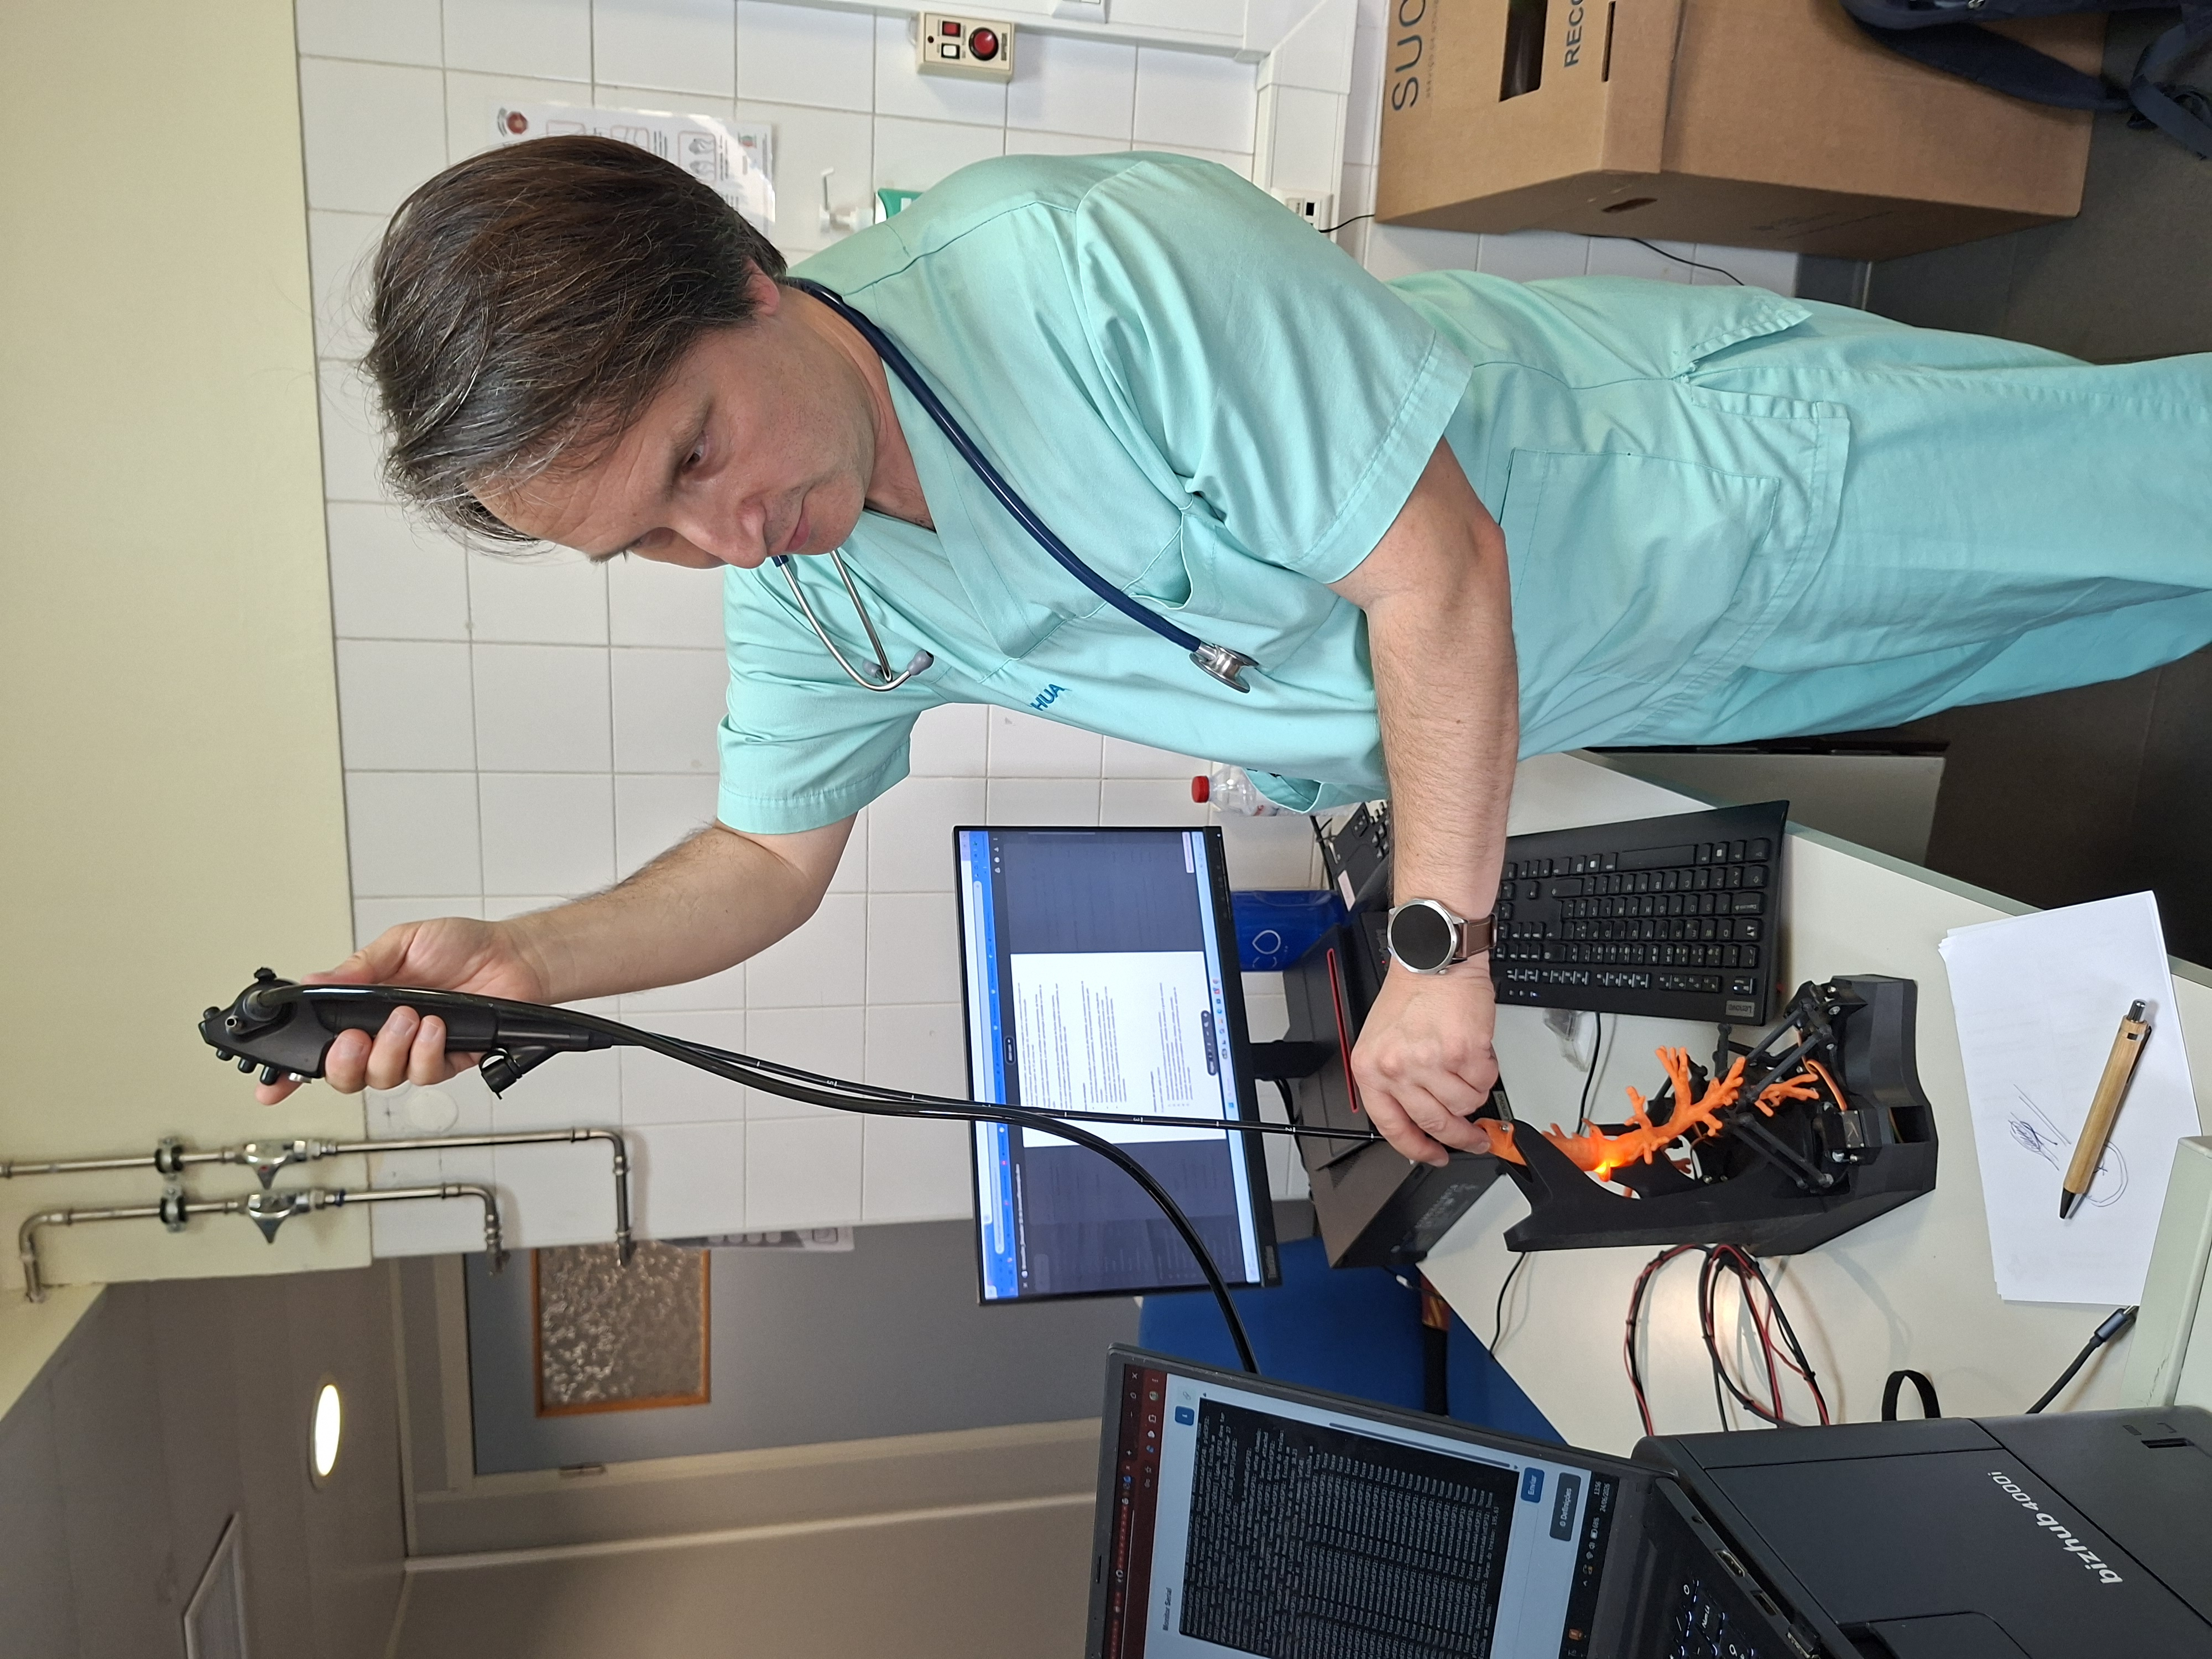
\includegraphics[width=0.82\textwidth]{fotos/teste_medico_broncoscopio.jpg}
  \caption{Sessão de observação preliminar com profissional de saúde: broncoscópio introduzido no modelo de árvore brônquica impresso em 3D enquanto o sistema de controlo estava ativo.}
  \label{fig:teste-medico}
\end{figure}

\section{Testes de integração dos movimentos}
A integração foi feita por etapas. Primeiro executou-se apenas a respiração, verificando periodicidade, amplitude e suavidade. Depois foi adicionado o batimento cardíaco, que deve aparecer como pequena oscilação sobreposta. Por fim, testou-se a tosse, que altera temporariamente o comportamento da respiração e ativa uma vibração ou perturbação curta.

O modo combinado é o mais importante para avaliar o realismo, pois aproxima o comportamento de um ambiente broncoscópico dinâmico. Neste modo, foram observados conflitos entre movimentos, saturação dos servos, perda de suavidade e eventuais posições impossíveis da cinemática inversa.

\chapter{Conclusão}

\section{Síntese do trabalho}
\begin{figure}[H]
  \centering
  \begin{subfigure}{0.48\textwidth}
    \centering
    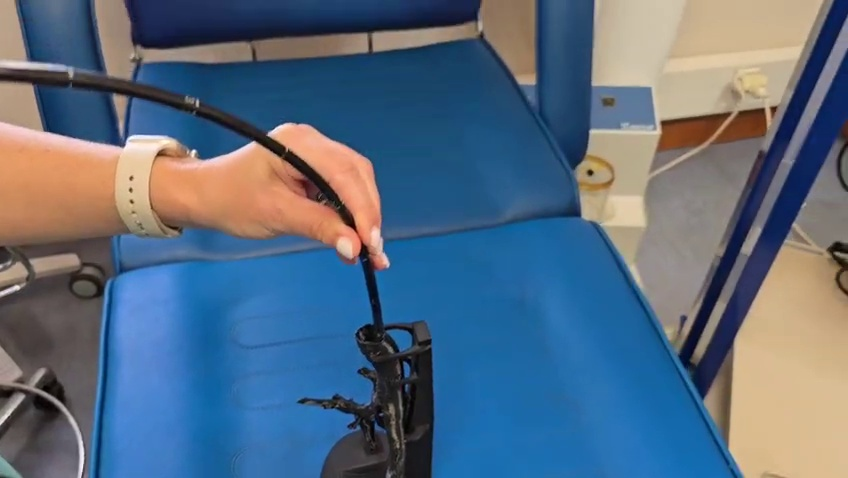
\includegraphics[width=\textwidth]{fotos/conclusao_inicio_modelo_video.jpg}
    \caption{Fase inicial de validação.}
  \end{subfigure}
  \hfill
  \begin{subfigure}{0.48\textwidth}
    \centering
    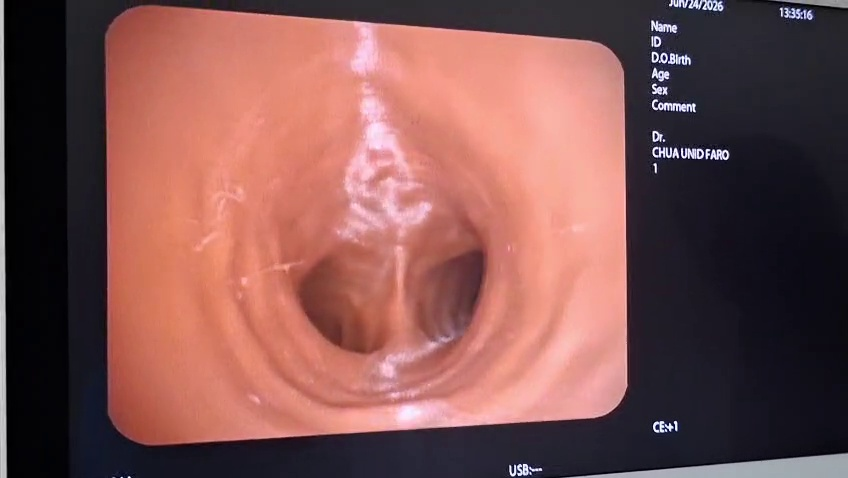
\includegraphics[width=\textwidth]{fotos/conclusao_final_modelo_video.jpg}
    \caption{Vista interna no ensaio final.}
  \end{subfigure}
  \caption{Comparação entre a validação inicial e o comportamento observado no modelo final.}
  \label{fig:comparacao-inicio-final-projeto}
\end{figure}

Este projeto teve como objetivo desenvolver um modelo físico e articulado de uma árvore brônquica para apoio ao treino de videobroncofibroscopia. A solução desenvolvida combinou a reconstrução anatómica a partir de dados clínicos, impressão 3D, atuação mecânica por manipuladores delta, controlo eletrónico com ESP32, comunicação com Raspberry Pi 4B, uma interface HMI e perfis de movimento inspirados em fenómenos fisiológicos observáveis durante o exame.

Ao longo do desenvolvimento, foi possível consolidar os requisitos principais do sistema e transformar uma ideia inicial ainda pouco definida num protótipo funcional, modular e capaz de reproduzir, de forma controlada, três movimentos considerados relevantes para a simulação: respiração, batimento cardíaco e tosse. A opção por manipuladores delta permitiu concentrar a atuação fora do modelo anatómico, evitando a instalação de motores diretamente na árvore brônquica e transferindo grande parte da flexibilidade do sistema para o software, através da geração de trajetórias e da cinemática inversa.

\begin{figure}[H]
  \centering
  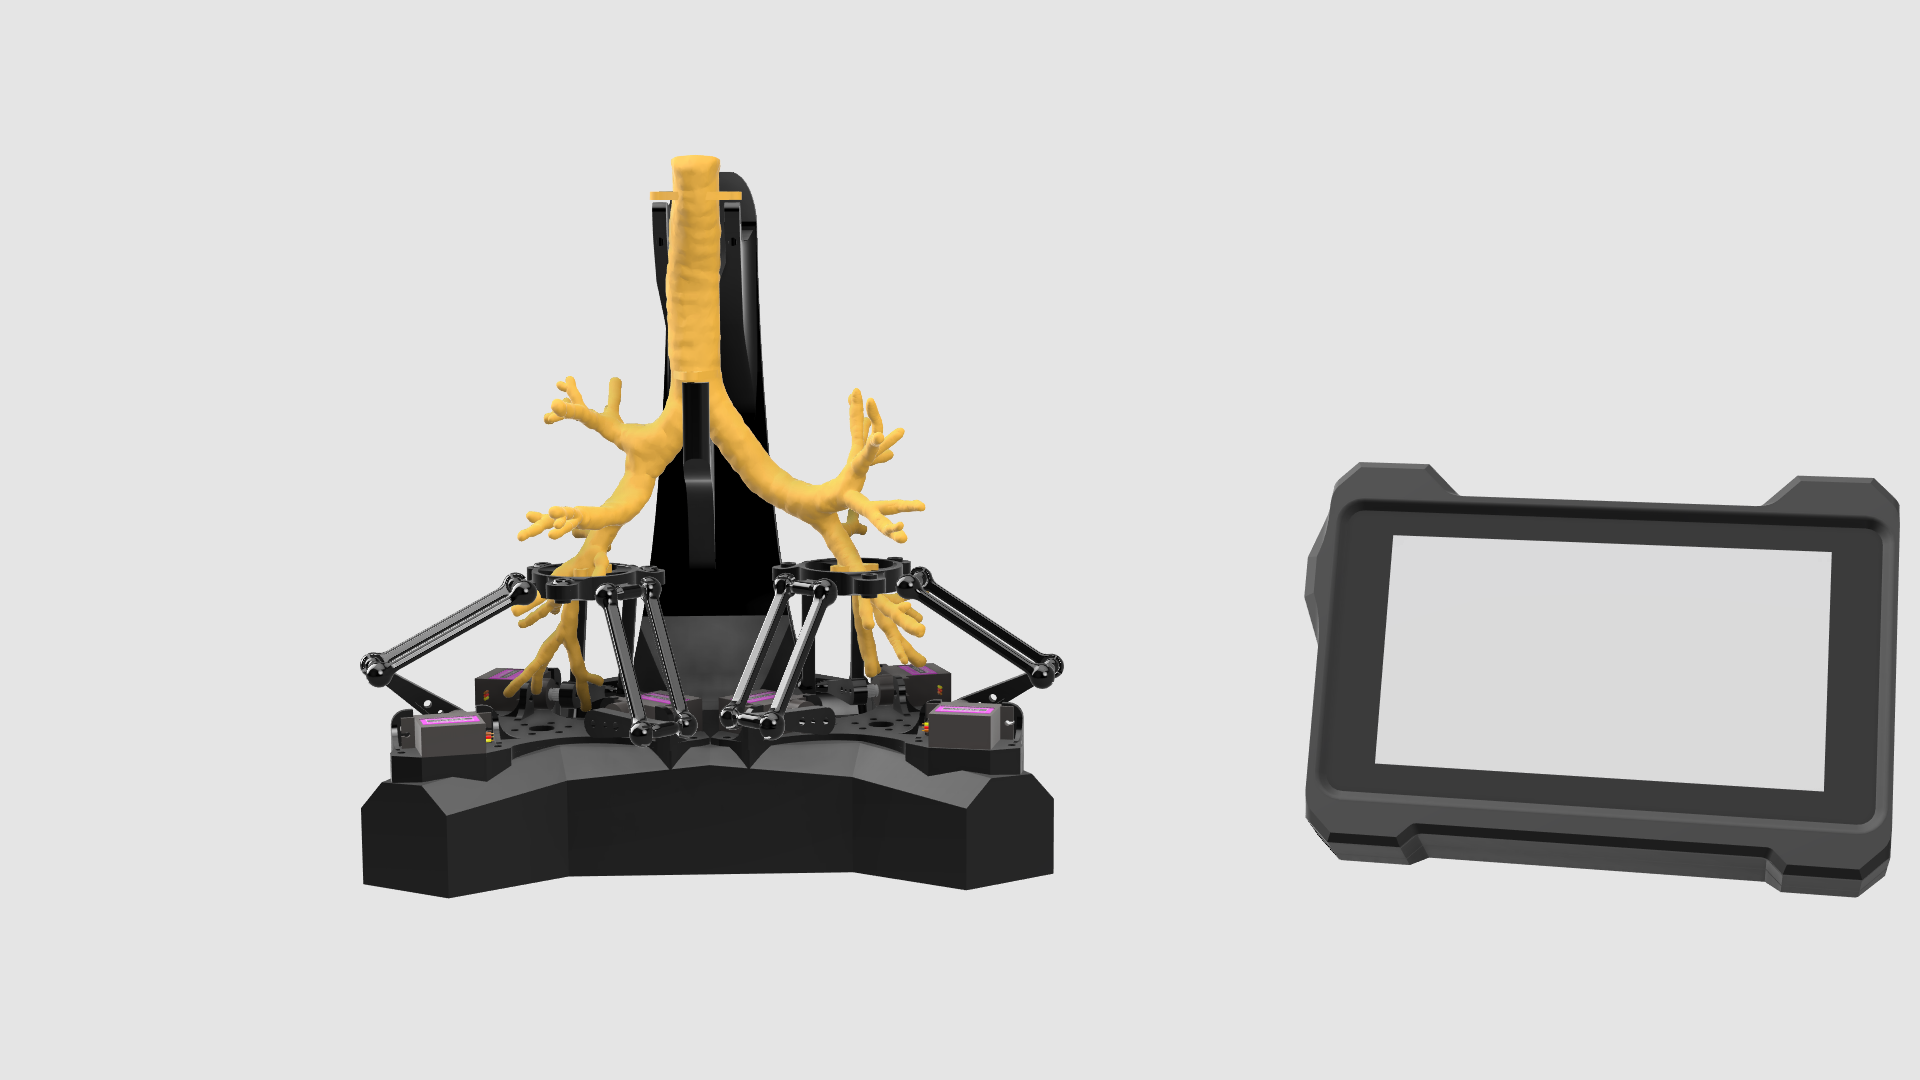
\includegraphics[width=0.82\textwidth]{fotos/cad_sistema_final.png}
  \caption{Representação CAD do conjunto final previsto.}
  \label{fig:cad-sistema-final-conclusao}
\end{figure}

Os ensaios laboratoriais permitiram caracterizar o comportamento do manipulador e avaliar a resposta temporal dos movimentos implementados. Embora tenham sido observadas discrepâncias entre os deslocamentos pretendidos e os deslocamentos obtidos, sobretudo em amplitudes maiores e em posições mais afastadas da zona central de trabalho, os resultados mostraram que o sistema era capaz de executar movimentos coerentes com os comandos aplicados. Nos testes de frequência, tanto o batimento cardíaco como a respiração acompanharam de forma consistente os valores configurados, confirmando a viabilidade da arquitetura de controlo adotada para os perfis fisiológicos previstos.

Os testes realizados com a equipa médica permitiram ainda validar qualitativamente a utilidade do modelo enquanto ferramenta de treino. A geometria da árvore brônquica foi considerada próxima da realidade anatómica e o comportamento dinâmico introduzido pelo sistema foi visto como um contributo relevante para aproximar o simulador de um ambiente broncoscópico real. O trabalho desenvolvido cumpriu, assim, o objetivo principal de demonstrar a viabilidade de um simulador físico, acessível e evolutivo, capaz de combinar anatomia impressa em 3D com movimento controlado.

\section{Limitações}
Apesar dos resultados obtidos, o protótipo apresentou limitações importantes. A primeira esteve relacionada com o próprio modelo impresso em 3D, que não foi concebido para lavagem interna. Esta limitação reduz a capacidade de reutilização em cenários onde seja necessário aplicar lubrificantes, introduzir líquidos ou simular procedimentos que exijam limpeza posterior do interior da árvore brônquica. Além disso, a geometria atual não permite ainda a colocação simples e controlada de objetos no interior do modelo, o que limita a simulação de corpos estranhos ou de situações clínicas mais específicas.

Outra limitação relevante esteve associada à precisão dos movimentos. Os servo-motores utilizados permitiram construir uma solução compacta e de baixo custo, mas não garantiram uma correspondência perfeita entre a posição calculada e o deslocamento real da plataforma. Esta diferença resulta da resolução e repetibilidade dos atuadores, das folgas mecânicas, da fricção nas juntas impressas e das próprias aproximações usadas na cinemática inversa. Em movimentos de pequena amplitude, estas discrepâncias foram menos críticas, mas tornaram-se mais visíveis em deslocamentos maiores ou próximos dos limites mecânicos.

Foi também observada a presença de vibrações e pequenas irregularidades, sobretudo em movimentos de baixa velocidade. Estas vibrações podem introduzir inconsistências na suavidade do movimento respiratório e alterar ligeiramente a perceção externa do comportamento do modelo. Embora, durante os testes clínicos, estas vibrações se tenham revelado menos evidentes na visão interna do broncoscópio do que na observação exterior, continuam a representar uma limitação importante para futuras versões que procurem maior fidelidade e repetibilidade.

Por fim, o protótipo ainda simplifica vários fenómenos presentes numa árvore traqueobrônquica real. O modelo não reproduz deformações locais do lúmen, variações de calibre ao longo do ciclo respiratório, estenoses dinâmicas, resistência ao contacto com o broncoscópio ou alterações provocadas diretamente pela interação entre o instrumento e as paredes internas. Estes aspetos foram identificados como relevantes, mas ficaram fora do âmbito desta versão devido à complexidade mecânica, material e de controlo que implicariam.

\section{Trabalho futuro}
Como trabalho futuro, poderá ser aprofundada a evolução do modelo físico da árvore brônquica, explorando novas tecnologias e materiais de impressão que permitam obter maior flexibilidade, melhor recuperação elástica e uma resposta mecânica mais próxima dos tecidos reais. Esta evolução poderá passar pela utilização de filamentos flexíveis com diferentes durezas, resinas elásticas, silicones ou processos híbridos de fabrico, procurando combinar uma geometria anatómica detalhada com paredes mais deformáveis e resistentes ao uso repetido.

Dentro dessa evolução construtiva, poderá também ser considerada a lavagem interna do modelo. Para esse efeito, seria útil introduzir soluções que facilitem a drenagem e reduzam a acumulação de resíduos no interior dos ramos, aproximando a utilização do simulador de condições de treino mais completas e aumentando a robustez do modelo em sessões repetidas.

Outra possibilidade de desenvolvimento será a introdução de objetos ou elementos substituíveis no interior da árvore brônquica, permitindo simular corpos estranhos, obstruções ou outros cenários clínicos. Esta capacidade tornaria o modelo mais versátil, sobretudo para médicos em fase inicial de aprendizagem, ao permitir exercícios de navegação, identificação e eventual remoção de elementos colocados em posições específicas.

No sistema de atuação e controlo, poderão ser otimizados tanto o firmware do ESP32 como a interface HMI. Do lado do firmware, futuras versões poderão melhorar a suavização dos movimentos, a calibração dos atuadores, a gestão de limites mecânicos e a sincronização entre respiração, batimento cardíaco e tosse. Do lado da HMI, poderá ser desenvolvida uma interface mais intuitiva e interativa, com melhor organização dos modos de treino, maior controlo sobre os parâmetros dos movimentos, armazenamento de perfis e uma visualização mais clara do estado interno do sistema.

Por último, poderá ser vantajoso melhorar as condições de avaliação e treino disponibilizadas aos médicos. Para além da validação qualitativa já iniciada, poderão ser definidos testes e exames mais estruturados para avaliar o modelo físico, envolvendo diferentes utilizadores, níveis de experiência e cenários clínicos. Esta etapa permitiria perceber com maior rigor que componentes do simulador têm maior valor pedagógico, que limitações afetam mais a experiência de utilização e que melhorias poderiam ser priorizadas para transformar o protótipo numa ferramenta de treino mais completa e clinicamente útil.


\nocite{*}
\printbibliography[heading=bibintoc,title={Bibliografia}]

\appendix
\cleardoublepage
\phantomsection
\addcontentsline{toc}{chapter}{Apêndice}
\chapter*{Apêndice}

\section*{Lista de materiais}
A \cref{tab:componentes-hardware} resume os componentes principais previstos para o sistema.

{\renewcommand{\thetable}{A.1}
\begin{table}[htbp]
  \centering
  \caption{Componentes principais previstos para o sistema.}
  \label{tab:componentes-hardware}
  \footnotesize
  \begin{tabular}{@{}>{\raggedright\arraybackslash}p{3.8cm}>{\raggedright\arraybackslash}p{3.2cm}>{\raggedright\arraybackslash}p{5.4cm}@{}}
    \toprule
    \textbf{Componente} & \textbf{Função} & \textbf{Observações} \\
    \midrule
    Raspberry Pi 4B & Interface e coordenação & Envia comandos ou posições para o ESP32 \\
    \rowcolor{gray!12}
    ESP32-S3 & Controlo dos atuadores & Executa FSMs e gera comandos para servos \\
    Servo-motores & Atuação mecânica & Seis unidades distribuídas pelos dois manipuladores delta \\
    \rowcolor{gray!12}
    Driver Servo-motores & Interface de potência/comando & Cada driver comanda três servo-motores de um manipulador delta \\
    UPS/HAT & Gestão de energia & Alimentação do Raspberry Pi e transição para bateria \\
    \rowcolor{gray!12}
    Fonte de Alimentação 5\,V--10\,A & Alimentação principal & Recebe 230\,V e fornece 5\,V ao sistema \\
    LiPo Battery 2100\,mA 3,7\,V & Alimentação de reserva & Bateria associada ao sistema UPS/HAT \\
    \bottomrule
  \end{tabular}
\end{table}}

\cleardoublepage
\phantomsection
\addcontentsline{toc}{chapter}{Anexos}
\chapter*{Anexos}

\section*{A.1\quad Desenhos técnicos e modelo 3D}
Incluir vistas do modelo, ficheiros CAD relevantes, parâmetros de impressão 3D e notas de montagem.

\section*{A.2\quad Código e configurações}
Incluir excertos relevantes de firmware, ficheiros de configuração, mapas de pinos e instruções de carregamento.


\end{document}
